% Document de classe yathesis, en 12 points, interligne un et demi, et version finale
\documentclass[12pt,space=onehalf,version=final]{yathesis}
%
% Chargement manuel de packages (pas déjà chargés par la classe yathesis)
\usepackage[T1]{fontenc}
\usepackage[utf8]{inputenc}
\usepackage{svg}
\usepackage{lipsum} % À proscrire dans un vrai mémoire de thèse !\
\usepackage{amsthm}
\usepackage{kpfonts}
\usepackage{algorithm2e}
\usepackage{booktabs}
\usepackage{siunitx}
\usepackage{pgfplots}
\usepackage{caption}
\usepackage{subcaption}
\usepackage{listings}
\usepackage{microtype}
\usepackage{varioref}
\usepackage[xindy,quiet]{imakeidx}
\usepackage[autostyle]{csquotes}
\usepackage[backend=biber,safeinputenc]{biblatex}
\usepackage{hyperref}
\usepackage[xindy,acronyms,symbols]{glossaries}
%
\newtheorem{definition}{Definition}
% Génération de l'index
\makeindex
%
% Spécification de la ou des ressources bibliographiques
\addbibresource{auxiliaires/bibliographie.bib}
\addbibresource{biblatex-examples.bib} % Fournie par biblatex.
%
% Génération du glossaire
\makeglossaries
%
% (Facultatif) Configuration des styles du glossaire et de la liste d'acronymes
% (à n'utiliser que si le package « glossaries » est chargé)
% \setglossarystyle{indexhypergroup}
% \setacronymstyle{long-sc-short}
%
% (Facultatif) Spécification de la ou des ressources terminologiques
% \loadglsentries{auxiliaires/glossaire}
% \loadglsentries{auxiliaires/acronymes}
% \loadglsentries{auxiliaires/symboles}
%
% Les réglages figurant habituellement dans le préambule, notamment concernant
% la bibliographie et l'éventuel index, peuvent être saisis dans le fichier
% « thesis.cfg » (situé dans le sous-dossier « configuration ») qui est
% automatiquement importé par la classe yathesis.
%
% Importation manuelle du fichier de macros personnelles
% % Macro pour mettre en forme les noms de fichiers
\newcommand{\fichier}[1]{\texttt{#1}}
% Macro pour mettre en forme les noms de packages LaTeX
\newcommand{\package}[1]{\textsf{#1}}
% Macro pour mettre en forme des locutions étrangères
\newcommand{\locution}[1]{\emph{#1}}


%
% Commande permettant de faire figurer d'un seul coup toutes les références des
% ressources bibliographiques ci-dessus, même si elles ne sont pas citées
% explicitement (à proscrire dans un vrai mémoire de thèse !)
\nocite{*}
%
%%%%%%%%%%%%%%%%%%%%%%%%%%%%%%%%%%%%%%%%%%%%%%%%%%%%%%%%%%%%%%%%%%%%%%%%%%%%%%%
%%%%%%%%%%%%%%%%%%%%%%%%%%%%%%%%%%%%%%%%%%%%%%%%%%%%%%%%%%%%%%%%%%%%%%%%%%%%%%%
% Début du document
%%%%%%%%%%%%%%%%%%%%%%%%%%%%%%%%%%%%%%%%%%%%%%%%%%%%%%%%%%%%%%%%%%%%%%%%%%%%%%%
%%%%%%%%%%%%%%%%%%%%%%%%%%%%%%%%%%%%%%%%%%%%%%%%%%%%%%%%%%%%%%%%%%%%%%%%%%%%%%%
\begin{document}
%
%%%%%%%%%%%%%%%%%%%%%%%%%%%%%%%%%%%%%%%%%%%%%%%%%%%%%%%%%%%%%%%%%%%%%%%%%%%%%%%
% Caractéristiques du document
%%%%%%%%%%%%%%%%%%%%%%%%%%%%%%%%%%%%%%%%%%%%%%%%%%%%%%%%%%%%%%%%%%%%%%%%%%%%%%%
%
% Préparation des pages de couverture et de titre
%%%%%%%%%%%%%%%%%%%%%%%%%%%%%%%%%%%%%%%%%%%%%%%%%%%%%%%%%%%%%%%%%%%%%%%%%%%%%%%
% Les caractéristiques de la thèse sont saisies dans le fichier
% « characteristics.tex » (situé dans le dossier « configuration »).
%
% Production des pages de couverture et de titre
%%%%%%%%%%%%%%%%%%%%%%%%%%%%%%%%%%%%%%%%%%%%%%%%%%%%%%%%%%%%%%%%%%%%%%%%%%%%%%%
\maketitle
%
%%%%%%%%%%%%%%%%%%%%%%%%%%%%%%%%%%%%%%%%%%%%%%%%%%%%%%%%%%%%%%%%%%%%%%%%%%%%%%%
% Début de la partie liminaire de la thèse
%%%%%%%%%%%%%%%%%%%%%%%%%%%%%%%%%%%%%%%%%%%%%%%%%%%%%%%%%%%%%%%%%%%%%%%%%%%%%%%
%
% (Facultatif) Production de la page de clause de non-responsabilité
% \makedisclaimer
%
% (Facultatif) Production de la page de mots clés
% \makekeywords
%
% (Facultatif) Production de la page affichant les logo, nom et coordonnées du
% ou des laboratoires (ou unités de recherche) où la thèse a été préparée
% \makelaboratory
%
% (Facultatif) Dédicace(s)
% % Dédicace(s)
\dedication{À mon directeur bien-aimé !}
\dedication{À mon co-directeur bien-co-aimé aussi !}
\dedication{Je dédie également ce travail\\à tous ceux qui le méritent}
% Production de la page de dédicace(s)
\makededications


%
% (Facultatif) Épigraphe(s)
% % Épigraphes(s)
\frontepigraph{Science sans conscience n'est que ruine de l'âme.}{François Rabelais}
\frontepigraph[english]{I can resist everything, except temptation!}{Oscar Wilde}
\frontepigraph{Il est plus facile de désintégrer un atome qu'un préjugé.}{Albert Einstein}
% Production de la page de d'épigraphe(s)
\makefrontepigraphs


%
% Résumés succincts
% Résumés (de 1700 caractères maximum, espaces compris) dans la
% langue principale (1re occurrence de l'environnement « abstract »)
% et, facultativement, dans la langue secondaire (2e occurrence de
% l'environnement « abstract »)
\begin{abstract}
  Dans cette thèse de doctorat, nous étudions des algorithmes d'apprentissage d'arbres de décision pour la classification supervisée et la prise de décision séquentielle. Les arbres de décision sont interprétables car les humains peuvent lire les opérations de l'arbre de décision depuis la racine jusqu'aux feuilles. Cela fait des arbres de décision le modèle de référence lorsque la vérification humaine est requise, comme dans les applications médicales. Cependant, les arbres de décision ne sont pas différentiables, ce qui les rend difficiles à optimiser, contrairement aux réseaux neuronaux qui peuvent être entraînés efficacement avec la descente de gradient. Les approches existantes d'apprentissage par renforcement interprétables apprennent généralement des arbres souples (non interprétables en l'état) ou sont ad hoc (entraînent un réseau neuronal puis entraînent un arbre à imiter le reseau). Cette apprentissage d'arbre indirect ne garantit pas de trouver des bonnes solutions pour le problème initial.

  Dans la première partie de ce manuscrit, nous visons à apprendre directement des arbres de décision pour un processus de décision Markovien avec de l'apprentissage par renforcement. En pratique, nous montrons que cela revient à résoudre un problème de décision Markovien partiellement observable (PDMPO). La plupart des algorithmes d'apprentissage par renforcement existants ne sont pas adaptés aux PDMPOs. Ce parallèle entre l'apprentissage des arbres de décision et la résolution des PDMPOs nous aide à comprendre pourquoi, dans la pratique, il est souvent plus facile d'obtenir une politique experte non interprétable (un réseau neuronal) puis de la distiller en un arbre plutôt que d'apprendre l'arbre de décision à partir de zéro.

  La deuxième contribution de ce travail découle de l'observation selon laquelle la recherche d'un arbre de décision est une instance complètement observable du problème précédent. Nous formulons donc l'induction d'arbres de décision comme la résolution d'un problème de décision Markovien et proposons un nouvel algorithme de pointe qui peut être entraîné à partir de données d'exemple supervisées et qui généralise bien à des données nouvelles.

  Les travaux des parties précédentes reposent sur l'hypothèse que les arbres de décision sont un modèle interprétable que les humains peuvent utiliser dans des applications sensibles. Mais est-ce vraiment le cas ? Dans la dernière partie de cette thèse, nous tentons de répondre à des questions plus générales sur l'interprétabilité: pouvons-nous mesurer l'interprétabilité sans intervention humaine ? Les arbres de décision sont-ils vraiment plus interprétables que les réseaux neuronaux ?

\end{abstract}
\begin{abstract}
  In this Ph.D. thesis, we study algorithms to learn decision trees for classification and sequential decision making. Decision trees are interpretable because humans can read through the decision tree computations from the root to the leaves. This makes decision trees the go-to model when human verification is required like in medicine applications. However, decision trees are non-differentiable making them hard to optimize unlike neural networks that can be trained efficiently with gradient descent. Existing interpretable reinforcement learning (RL) approaches usually learn soft trees (non-interpretable as is) or are ad-hoc (train a neural network then fit a tree to it) potentially missing better solutions.

  In the first part of this manuscript, we aim to directly learn decision trees for a Markov decision process with reinforcement learning. In practice we show that this amounts to solving a partially observable Markov decision problem (POMDP). Most existing RL algorithms are not suited for POMDPs. This parallel between decision tree learning with RL and POMDPs solving help us understand why in practice it is often easier to obtain a non-interpretable expert policy--a neural network--and then distillate it into a tree rather than learning the decision tree from scratch.

  The second contribution from this work arose from the observation that looking for a decision tree classifier (or regressor) is a fully observable instance of the above problem. We thus formulate decision tree induction as sloving a Markov decision problem and propose a new state-of-the-art algorithm that can be trained with supervised example data and generalizes well to unseen data.

  Work from the previous parts rely on the hypothesis that decision trees are indeed an interpretable model that humans can use in sensitive applications. But is it really the case? In the last part of this thesis, we attempt to answer some more general questions about interpretability: can we measure interpretability without humans? And are decision trees really more interpretable than neural networks?
\end{abstract}
%
% Production de la page de résumés
\makeabstract{}


%
% (Facultatif) Chapitre de remerciements
% \chapter{Remerciements}
\section{Une section de remerciements}
\lipsum[1]
\section{Une autre section de remerciements}
\lipsum[2-9]


%
% (Facultatif) Chapitre d'avertissement
% \chapter{Avertissement}
Thèse hilarante, comme le gaz du même nom !


%
% (Facultatif) Liste des acronymes
% \printacronyms
%
% (Facultatif) Liste des symboles
% \printsymbols
%
% (Facultatif) Chapitre d'avant-propos
% \chapter{Avant-propos}
\section{Une section d'avant-propos}
\lipsum[30-45]
\section{Une autre section d'avant-propos}
\lipsum[30-35]


%
% Sommaire
\tableofcontents[depth=chapter,name=Sommaire]
%
% (Facultatif) Liste des tableaux
% \listoftables
%
% (Facultatif) Table des figures
% \listoffigures
%
% (Facultatif) Table des listings (nécessite que le package « listings » soit
% chargé)
% \lstlistoflistings
%
%%%%%%%%%%%%%%%%%%%%%%%%%%%%%%%%%%%%%%%%%%%%%%%%%%%%%%%%%%%%%%%%%%%%%%%%%%%%%%%
% Début de la partie principale (du « corps ») de la thèse
%%%%%%%%%%%%%%%%%%%%%%%%%%%%%%%%%%%%%%%%%%%%%%%%%%%%%%%%%%%%%%%%%%%%%%%%%%%%%%%
\mainmatter
%
% Chapitre d'introduction (générale)
%%%%%%%%%%%%%%%%%%%%%%%%%%%%%%%%%%%%%%%%%%%%%%%%%%%%%%%%%%%%%%%%%%%%%%%%%%%%%%%
\chapter*{Preliminary Concepts}
\section{What is sequential decision making?}\label{sec:intro-sdm}
\begin{figure}
    \centering
    \begin{tikzpicture}[
        node distance=2.5cm,
        auto,
        thick,
        state/.style={circle, draw, fill=blue!20, minimum size=1.5cm, text centered},
        environment/.style={rectangle, draw, dashed, fill=blue!10, rounded corners, minimum width=4cm, minimum height=2cm, text centered},
        agent/.style={rectangle, draw, fill=orange!20, rounded corners, minimum width=2cm, minimum height=1.5cm, text centered},
        robot/.style={rectangle, draw, fill=green!20, rounded corners, minimum width=2cm, minimum height=1.5cm, text centered},
        decision_box/.style={rectangle, draw, dashed, fill=gray!10, minimum width=7.5cm, minimum height=3cm, text centered},
        arrow/.style={->, thick, bend left=15},
        arrow_decision/.style={->, dashed, bend left=15}
    ]
        
        % Decision Making Box
        \node[decision_box] (decision_box) at (0.3,3.4) {};
        \node at (0.3,4.5) {\small{Decision Making}};
        
        % Robot (AI)
        \node[robot] (robot) at (-2.1,3.2) {
            \begin{minipage}{1.5cm}
                \centering
                \includesvg[width=0.4cm]{images/images_intro/robot-svgrepo-com.svg}\\
                \small{Computer program}
            \end{minipage}
        };
        
        % Doctor
        \node[agent] (doctor) at (2.5,3.2) {
            \begin{minipage}{1.5cm}
                \centering
                \includesvg[width=0.4cm]{images/images_intro/doctor-with-stethoscope-svgrepo-com.svg}\\
                \small{Doctor}
            \end{minipage}
        };
        
        % Environment (Patient)
        \node[environment] (environment) at (0,-0.5) {
            \begin{minipage}{2cm}
                \centering
                \includesvg[width=0.8cm]{images/images_intro/patient-4.svg}\\
                \small{Cancer patient}
            \end{minipage}
        };
        
        % Arrows
        \draw[arrow] (environment) to[bend left=30] node[left] {
            \begin{minipage}{2cm}
                \centering
                \includesvg[width=0.4cm]{images/images_intro/patient-clipboard-svgrepo-com.svg}\\
                \small{Updated health status}
            \end{minipage}
        } (robot);
        \draw[arrow_decision] (robot) to node[above] {\small{Recommends}} (doctor);
        \draw[arrow_decision] (doctor) to node[below] {\small{Interprets}} (robot);

        \draw[arrow] (doctor) to[bend left=30] node[right] {
            \begin{minipage}{1.5cm}
                \centering
                \includesvg[width=0.5cm]{images/images_intro/syringe-svgrepo-com.svg}\\
                \small{Administer chemotherapy}
            \end{minipage}
        } (environment);
        
    \end{tikzpicture}
    \caption{Sequential decision making in cancer treatment. The AI system reacts to the patient's current state (tumor size, blood cells counts, etc.) and makes a recommendation to the doctor, who administers chemotherapy to the patient. The patient's state is then updated, and this cycle repeats over time.}
    \label{fig:cancer-treatment-sdm}
\end{figure}
In this manuscript, we study algorithms for sequential decision making. Humans engage in sequential decision making in all aspects of life. In medicine, doctors have to decide how much chemotherapy to administer based on the patient's current health~\cite{cancer}. In agriculture, agronomists have to decide when to fertilize based on the current soil and weather conditions to maximize plant growth~\cite{agriculture}. 
In automotive settings, the autopilot system has to decide how to steer based on lidar and other sensors to maintain a safe trajectory~\cite{driving}. 
These sequential decision making processes exhibit key similarities: an agent takes actions based on current information to achieve a goal.

As computer scientists, we ought to design computer programs~\cite{knuth63} that can help humans during these sequential decision making processes. 
For example, as depicted in figure~\ref{fig:cancer-treatment-sdm}, a doctor could benefit from a program that would recommend the ``best'' treatment given the patient's state. 
Machine learning algorithms~\cite{turing} output such helpful programs.
For non-sequential decision making, when the doctor only takes one decision and does not need to react to the updated patient's health, e.g. making a diagnosis about cancer type, a program can be fitted to example data: given lots of patient records and the associated diagnoses, the program learns to make the same diagnosis a doctor would given the same patient record, this is \textit{supervised} learning~\cite{sl}. 
In the cancer treatment example, the doctor follows the patient over time and adapts treatment to the patient's changing health. In that case, machine learning—and in particular \textit{reinforcement} learning (RL)~\cite{sutton}—can be used to teach the program how to take decisions that lead to recovery based on how the patient's health changes from one dose to another.  
Such machine learning algorithms train increasingly performant programs that are deployed to, e.g., identify digits in images~\cite{lenet}, control tokamak fusion~\cite{tokamak}, or write the abstract of a scientific article~\cite{reinforce-llm}.

However, the computations performed by these programs cannot be understood and verified by humans: the programs are black-box.
This can be problematic in applications where decisions have important consequences. 
Consider the following extreme scenario in the context of the cancer treatment example: a program recommends to the doctor to amputate a patient's limb.
While amputating could be the only way to save the patient's life, it is not hard to imagine that such an extreme recommendation would not be followed by the doctor unless it comes with convincing explanations or unless the factors that influenced the program's recommendation can be presented to the doctor. 
In an other setting where the program directly act in the real-world, i.e. it does not make recommendations to a human but rather acts autonomously, black-box programms are also not desirable.
Consider the slightly extreme scenario of a combat drone in which a program decides on who to shoot.
In this context, it is hard to imagine leaders deploying such drones and programs without having strict guarantees that it will, e.g. not shoot civilians.
Such guarantees can be obtained through formal verifications of programs which in turn can only be obtain for certain programs.

Next, we describe the notion of interpretability that is key to ensure that programs can be verified and their recommendations can be understood.

\section{What is Interpretability?}


Originally, the etymology of ``interpretability'' is the Latin ``interpretabilis'', meaning ``that can be understood and explained''.
According to the Oxford English Dictionary, the first recorded use of the English word ``interpretability'' dates back to 1854, when the British logician George Boole (figure~\ref{fig:george-boole}) described the addition of concepts:

\begin{displaycquote}[p.~48]{boole}
I would remark in the first place that the generality of a method in Logic
must very much depend upon the generality of its elementary processes and laws.
We have, for instance, in the previous sections of this work investigated, among
other things, the laws of that logical process of addition which is symbolized by
the sign +. Now those laws have been determined from the study of instances,
in all of which it has been a necessary condition, that the classes or things added
together in thought should be mutually exclusive. The expression x + y seems
indeed uninterpretable, unless it be assumed that the things represented by x
and the things represented by y are entirely separate; that they embrace no
individuals in common. And conditions analogous to this have been involved
in those acts of conception from the study of which the laws of the other
symbolical operations have been ascertained. The question then arises, whether
it is necessary to restrict the application of these symbolical laws and processes
by the same conditions of interpretability under which the knowledge of them
was obtained. If such restriction is necessary, it is manifest that no such thing
as a general method in Logic is possible. On the other hand, if such restriction
is unnecessary, in what light are we to contemplate processes which appear to
be uninterpretable in that sphere of thought which they are designed to aid?
\end{displaycquote}\label{quote:boole}

\begin{figure}
    \centering
    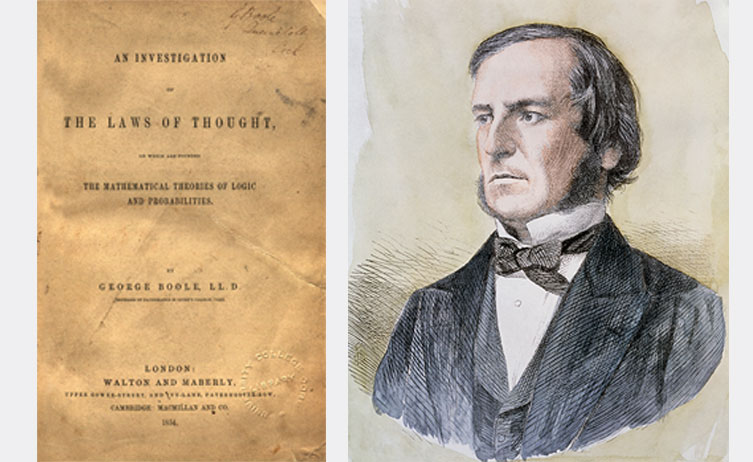
\includegraphics[width=0.5\textwidth]{images/images_intro/gboole.jpg}
    \caption{British logician and philosopher George Boole (1815--1864) next to his book \textit{The Laws of Thought} (1854), the oldest known record of the word ``interpretability''.}
    \label{fig:george-boole}
\end{figure}

What is remarkable is that the first recorded occurrence of ``interpretability'' was in the context of logic and computation. 
In Boole's system, the expression $x+y$ is interpretable only when $x$ and $y$ are disjoint sets, because then ``+'' clearly represents their union. 
By contrast, in e.g. a neural network program~\cite{perceptron}, an operation like $x+y$ typically means adding two hidden vectors in a high-dimensional space. 
The result is mathematically well-defined, but its semantic meaning—what concept or feature this new vector corresponds to—is black-box. 
Just as Boole worried that logic would lose its generality and practical use if restricted only to easily interpretable operations, there exisits similar tension in machine learning today.
In machine learning, should we limit ourselves to inherently interpretable programs (like decision trees~\cite{breiman1984classification}, where $x+y$ might literally mean combining two feature contributions, like blood cells count and tumor size) or accept uninterpretable computations in black-box programs (like in neural networks) in order to have boradly applicable and highly performant programs?
The global trend in machine learning research answers the latter.

\begin{figure}
    \centering
    \begin{subfigure}[b]{0.7\textwidth}
        \centering
        \begin{tikzpicture}[
            node distance=2.5cm,
            auto,
            thick,
            state/.style={circle, draw, fill=blue!20, minimum size=1.5cm, text centered},
            environment/.style={rectangle, draw, dashed, fill=blue!10, rounded corners, minimum width=4cm, minimum height=2cm, text centered},
            agent/.style={rectangle, draw, fill=orange!20, rounded corners, minimum width=2cm, minimum height=1.5cm, text centered},
            robot/.style={rectangle, draw, fill=black!20, rounded corners, minimum width=2cm, minimum height=1.5cm, text centered},
            ml/.style={circle, draw, fill=purple!20, minimum width=2cm, minimum height=1cm, text centered},
            decision_box/.style={rectangle, draw, dashed, fill=gray!10, minimum width=7.5cm, minimum height=3cm, text centered},
            arrow/.style={->, thick, bend left=15},
            arrow_decision/.style={->, dashed, bend left=15}
        ]
            
            % Decision Making Box
            \node[decision_box] (decision_box) at (0.3,3.4) {};
            \node at (0.3,4.5) {\small{Decision Making}};
            
            % Robot (AI)
            \node[robot] (robot) at (-2.1,3.2) {
                \begin{minipage}{1.5cm}
                    \centering
                    \includesvg[width=0.4cm]{images/images_intro/network-mapping-svgrepo-com.svg}\\
                    \small{Neural network}
                \end{minipage}
            };
            
            % Doctor
            \node[agent] (doctor) at (2.5,3.2) {
                \begin{minipage}{1.5cm}
                    \centering
                    \includesvg[width=0.4cm]{images/images_intro/doctor-with-stethoscope-svgrepo-com.svg}\\
                    \small{Doctor}
                \end{minipage}
            };
            
            % Machine Learning component
            \node[ml] (ml) at (-7,3) {
                \begin{minipage}{1.8cm}
                    \centering
                    \includesvg[width=0.4cm]{images/images_intro/gear-file-svgrepo-com.svg}\\
                    \small{Machine learning}
                \end{minipage}
            };
            
            % Environment (Patient)
            \node[environment] (environment) at (0,-0.5) {
                \begin{minipage}{2cm}
                    \centering
                    \includesvg[width=0.8cm]{images/images_intro/patient-4.svg}\\
                    \small{Cancer patient}
                \end{minipage}
            };
            
            % Arrows
            \draw[arrow] (environment) to[bend left=30] node[left] {
                \begin{minipage}{2cm}
                    \centering
                    \includesvg[width=0.5cm]{images/images_intro/patient-clipboard-svgrepo-com.svg}\\
                    \small{Updated health status}
                \end{minipage}
            } (robot);
            \draw[arrow_decision] (robot) to node[above] {\small{Recommends}} (doctor);
            \draw[arrow_decision, red] (doctor) to node[below] {\small{Cannot interpret}} (robot);
            
        \draw[arrow] (doctor) to[bend left=30] node[right] {
                \begin{minipage}{1.5cm}
                    \centering
                    \includesvg[width=0.5cm]{images/images_intro/syringe-svgrepo-com.svg}\\
                \small{Administer chemotherapy}
                \end{minipage}
            } (environment);
            
            % ML learning arrows
            \draw[arrow] (environment) to[bend left=40] node[left] {
                \begin{minipage}{2cm}
                    \centering
                    \includesvg[width=0.5cm]{images/images_intro/patient-clipboard-svgrepo-com.svg}\\
                    \small{Treatment outcomes}
                \end{minipage}
            } (ml);
            \draw[arrow] (ml) to[bend left=20] node[above] {
                \begin{minipage}{1.5cm}
                    \centering
                    \small{Updates program}
                \end{minipage}
            } (robot);
            
        \end{tikzpicture}
        \caption{Black-box approach using neural networks}
        \label{fig:cancer-treatment-sdm-ml}
    \end{subfigure}
    
    \vspace*{1cm}
    
    \begin{subfigure}[b]{0.7\textwidth}
        \centering
        \begin{tikzpicture}[
            node distance=2.5cm,
            auto,
            thick,
            state/.style={circle, draw, fill=blue!20, minimum size=1.5cm, text centered},
            environment/.style={rectangle, draw, dashed, fill=blue!10, rounded corners, minimum width=4cm, minimum height=2cm, text centered},
            agent/.style={rectangle, draw, fill=orange!20, rounded corners, minimum width=2cm, minimum height=1.5cm, text centered},
            robot/.style={rectangle, draw, fill=green!20, rounded corners, minimum width=2cm, minimum height=1.5cm, text centered},
            ml/.style={circle, draw, fill=purple!20, minimum width=2cm, minimum height=1cm, text centered},
            decision_box/.style={rectangle, draw, dashed, fill=gray!10, minimum width=7.5cm, minimum height=3cm, text centered},
            arrow/.style={->, thick, bend left=15},
            arrow_decision/.style={->, dashed, bend left=15}
        ]
            
            % Decision Making Box
            \node[decision_box] (decision_box) at (0.3,3.4) {};
            \node at (0.3,4.5) {\small{Decision Making}};
            
            % Robot (AI)
            \node[robot] (robot) at (-2.1,3.2) {
                \begin{minipage}{1.5cm}
                    \centering
                    \includesvg[width=0.4cm]{images/images_intro/decision-tree-svgrepo-com.svg}\\
                    \small{Decision tree}
                \end{minipage}
            };
            
            % Doctor
            \node[agent] (doctor) at (2.5,3.2) {
                \begin{minipage}{1.5cm}
                    \centering
                    \includesvg[width=0.4cm]{images/images_intro/doctor-with-stethoscope-svgrepo-com.svg}\\
                    \small{Doctor}
                \end{minipage}
            };
            
            % Machine Learning component
            \node[ml] (ml) at (-7,3) {
                \begin{minipage}{1.8cm}
                    \centering
                    \includesvg[width=0.4cm]{images/images_intro/gear-file-svgrepo-com.svg}\\
                    \small{Interpretable machine learning}
                \end{minipage}
            };
            
            % Environment (Patient)
            \node[environment] (environment) at (0,-0.5) {
                \begin{minipage}{2cm}
                    \centering
                    \includesvg[width=0.8cm]{images/images_intro/patient-4.svg}\\
                    \small{Cancer patient}
                \end{minipage}
            };
            
            % Arrows
            \draw[arrow] (environment) to[bend left=30] node[left] {
                \begin{minipage}{2cm}
                    \centering
                    \includesvg[width=0.5cm]{images/images_intro/patient-clipboard-svgrepo-com.svg}\\
                    \small{Updated health status}
                \end{minipage}
            } (robot);
            \draw[arrow_decision] (robot) to node[above] {\small{Recommends}} (doctor);
            \draw[arrow_decision, green] (doctor) to node[below] {\small{Can interpret}} (robot);
            
            \draw[arrow] (doctor) to[bend left=30] node[right] {
                \begin{minipage}{1.5cm}
                    \centering
                    \includesvg[width=0.5cm]{images/images_intro/syringe-svgrepo-com.svg}\\
                    \small{Administer chemotherapy}
                \end{minipage}
            } (environment);
            
            % ML learning arrows
            \draw[arrow] (environment) to[bend left=40] node[left] {
                \begin{minipage}{2cm}
                    \centering
                    \includesvg[width=0.5cm]{images/images_intro/patient-clipboard-svgrepo-com.svg}\\
                    \small{Treatment outcomes}
                \end{minipage}
            } (ml);
            \draw[arrow] (ml) to[bend left=20] node[above] {
                \begin{minipage}{1.5cm}
                    \centering
                    \small{Updates program}
                \end{minipage}
            } (robot);
            
        \end{tikzpicture}
        \caption{Interpretable approach using decision trees}
        \label{fig:cancer-treatment-comparison}
    \end{subfigure}
    \caption{Comparison of sequential decision making approaches in cancer treatment. Top: a black-box neural network approach where the doctor cannot interpret the AI's recommendations because the computations are operations over uninterpretable concepts (cf. end of section~\ref{sec:intro-sdm} and Boole's quote~\ref{quote:boole}). Bottom: an interpretable decision tree approach where the doctor can understand and verify the AI's recommendations because the operations are perfomed over meaningful concepts  (cf. end of section~\ref{sec:intro-sdm} and Boole's quote~\ref{quote:boole}). Both systems learn from treatment outcomes to improve their recommendations over time.}
    \label{fig:cancer-treatment-comparison-combined}
\end{figure}

In figure~\ref{fig:cancer-treatment-sdm-ml}, we illustrate how existing machine learning algorithms \textit{could} be used in principle to help with cancer treatment. In truth, this should be prohibited without some kind of transparency in the program's recommendation: why did the program recommend such a dosage?
In figure~\ref{fig:cancer-treatment-comparison}, we illustrate how machine learning \textit{should} be used in practice. 
Ideally, we want doctors to have access to computer programs that can recommend ``good'' treatments and whose recommendations are interpretable. 
In the next section, present related works that fit this desiderata.

\section{What are existing approaches for learning interpretable programs?}\label{sec:intro-interp}

In this section we follow sections 6 and 7 of \cite{glanois-survey} and section 5 of \cite{milani-survey}. 
Furthermore we now employ the term ``model'' to refer to ``programs'' to be consistent with the machine learning research conventions.
Models are essentially mappings from inputs to outputs that can be trained with machine learning algorithms while programs might designate other types of computations like \texttt{print("Hello World");}.

\begin{figure}
    \centering
    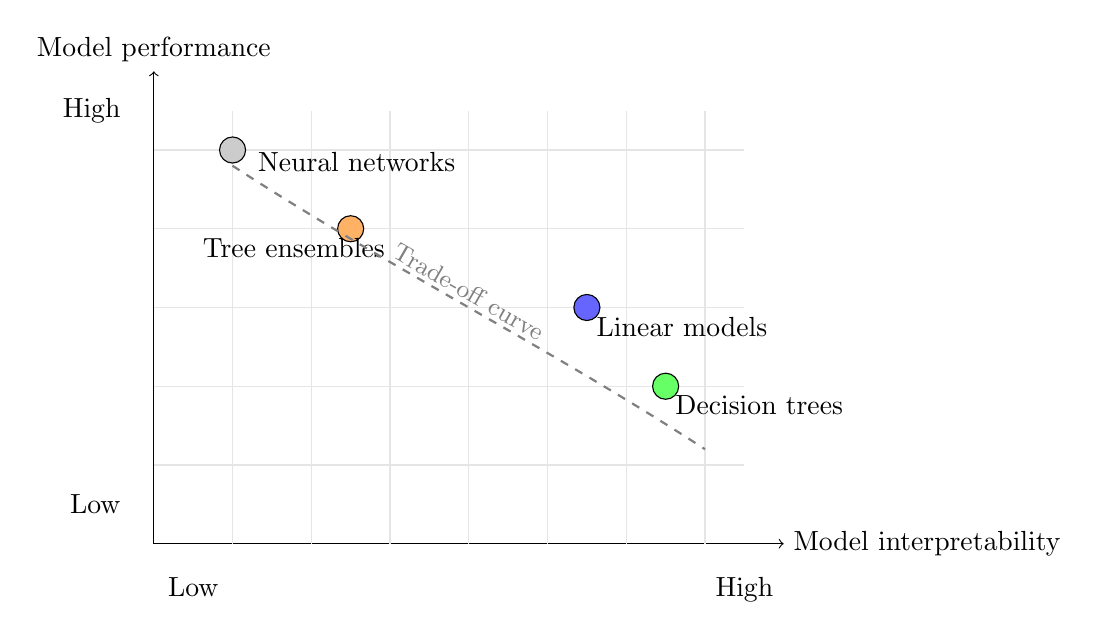
\begin{tikzpicture}
        % Define the axes
        \draw[->] (0,0) -- (8,0) node[right] {Model interpretability};
        \draw[->] (0,0) -- (0,6) node[above] {Model performance};
        
        % Add axis labels at the ends
        \node[below] at (0.5,-0.3) {Low};
        \node[below] at (7.5,-0.3) {High};
        \node[left] at (-0.3,0.5) {Low};
        \node[left] at (-0.3,5.5) {High};
        
        % Add grid lines (optional, subtle)
        \foreach \x in {1,2,...,7}
            \draw[gray!20] (\x,0) -- (\x,5.5);
        \foreach \y in {1,2,...,5}
            \draw[gray!20] (0,\y) -- (7.5,\y);
            
        % Position different model types
        % Deep Neural Networks (high performance, low interpretability)
        \node[circle, fill=black!20, draw, minimum size=8pt] at (1,5) {};
        \node[below right] at (1.2,5.1) {Neural networks};
        
        % Ensemble Methods (medium-high performance, low-medium interpretability)
        \node[circle, fill=orange!60, draw, minimum size=8pt] at (2.5,4) {};
        \node[below right] at (0.5,4) {Tree ensembles};
        
        % Linear Models (medium performance, high interpretability)
        \node[circle, fill=blue!60, draw, minimum size=8pt] at (5.5,3) {};
        \node[below right] at (5.5,3) {Linear models};
        
        % Decision Trees (medium-low performance, high interpretability)
        \node[circle, fill=green!60, draw, minimum size=8pt] at (6.5,2) {};
        \node[below right] at (6.5,2) {Decision trees};
        

        
        % Add a general trend line (optional)
        \draw[dashed, thick, gray] (1,4.8) .. controls (3,3.5) and (5,2.5) .. (7,1.2);
        \node[gray, rotate=-30] at (4,3.2) {\small Trade-off curve};
        
    \end{tikzpicture}
    \caption{The interpretability–performance trade-off in machine learning. Different model classes are positioned according to their typical interpretability and performance characteristics. The dashed line illustrates the general trade-off between these two properties.}
    \label{fig:interpretability-performance-tradeoff}
\end{figure}
Interpretable machine learning provides either local or global interpretations \cite{glanois-survey}.
Global methods, like decision tree induction~\cite{breiman1984classification}, return a model whose outputs can be interpreted without having to run an additional algorithm.
By contrast, local methods require to run an additional algorithm, e.g. linear regression~\cite{regression}, but are agnostic to the model class.
In figure~\ref{fig:interpretability-performance-tradeoff} we present a popular trade-off between interpretability and performance of different model classes based on various user studies and popular beliefs~\cite{study-0,study-1,study-2,study-3,study-4,study-5,study-6,study-7}.

Local interpretable model-agnostic explanations (LIME)~\cite{lime} is a popular local interpretablity method.
Given a model, LIME works by perturbing the input and learning a simple interpretable model locally to explain that particular prediction (see figure~\ref{fig:lime}). 
For each individual prediction, LIME provides interpretations by identifying which features were most important for that specific decision.

Local interpretability can also be called explainability.
Global interpretability methods constrain the model class so that the computations are transparent or verifiable by construction. 
On the other hand, explainability methods--or local interpretability methods--keep black-box models and generates post hoc explanations of their decisions. 
In additions to linear models, explanations can take various forms: visual explanations with saliency maps \cite{Puri2020Explain}, attribution such as SHAP\cite{shap}, attention-based highlighting \cite{attention}.

While useful for insight, these explanations are often subjective and might not be faithful to the underlying computations~\cite{Atrey2020Exploratory}.
For safety-critical settings, this motivates our focus on models that are interpretable by design.
Those interpretable by design models can be obtained by global interpretability methods that we present next.

\begin{figure}
    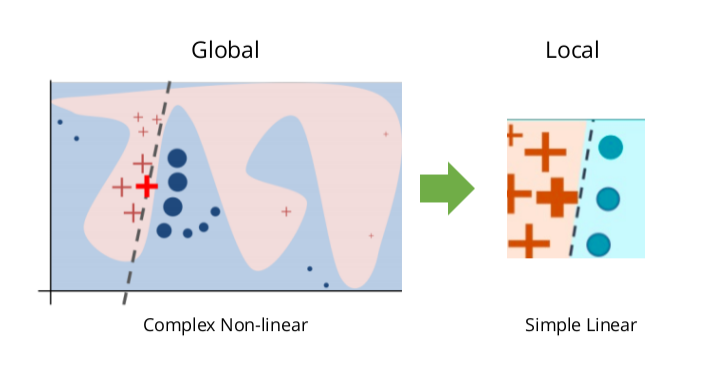
\includegraphics[width=0.9\textwidth]{images/lime.png}
    \caption{Local Interpretable Model-agnostic Explanations~\cite{lime} fit an interpretable linear model to data around the red cross prediction to be interpreted.}\label{fig:lime}
\end{figure}


\begin{figure}
    \centering
    \begin{tikzpicture}[
        node distance=2cm,
        auto,
        thick,
        rl/.style={circle, draw, fill=purple!20, minimum width=1.5cm, minimum height=0.8cm, text centered},
        nn/.style={rectangle, draw, fill=black!20, rounded corners, minimum width=1.5cm, minimum height=1cm, text centered},
        sl/.style={circle, draw, fill=blue!20, minimum width=1.5cm, minimum height=0.8cm, text centered},
        dt/.style={rectangle, draw, fill=green!20, rounded corners, minimum width=1.5cm, minimum height=1cm, text centered},
        arrow/.style={->, thick},
        label/.style={font=\tiny, above},
        method_box/.style={rectangle, draw, dashed, minimum width=5cm, minimum height=3cm, text centered},
        method_box_indirect/.style={rectangle, draw, dashed, minimum width=9.5cm, minimum height=3cm, text centered}
    ]
        
        % Direct method box
        \node[method_box] (direct_box) at (-0.5,0) {};
        \node at (-0.5,1.7) {\small{Direct}};
        
        % Direct method - RL process
        \node[rl] (rl_direct) at (-2,0) {
            \begin{minipage}{1.2cm}
                \centering
                \includesvg[width=0.3cm]{images/images_intro/gear-file-svgrepo-com.svg}\\
                \tiny{Reinforcement learning}
            \end{minipage}
        };
        
        % Direct method - Decision Tree
        \node[dt] (dt_direct) at (1,0) {
            \begin{minipage}{1.2cm}
                \centering
                \includesvg[width=0.3cm]{images/images_intro/decision-tree-svgrepo-com.svg}\\
                \tiny{Decision tree}
            \end{minipage}
        };
        
        % Direct method arrow
        \draw[arrow] (rl_direct) -- (dt_direct) node[label, midway] {\tiny Learns};
        
        % Indirect method box
        \node[method_box_indirect] (indirect_box) at (7.1,0) {};
        \node at (6.8,1.7) {\small{Indirect}};
        
        % Indirect method - RL process
        \node[rl] (rl_indirect) at (3.5,0) {
            \begin{minipage}{1.2cm}
                \centering
                \includesvg[width=0.3cm]{images/images_intro/gear-file-svgrepo-com.svg}\\
                \tiny{Reinforcement learning}
            \end{minipage}
        };
        
        % Indirect method - Neural Network
        \node[nn] (nn_indirect) at (6,0) {
            \begin{minipage}{1.2cm}
                \centering
                \includesvg[width=0.3cm]{images/images_intro/network-mapping-svgrepo-com.svg}\\
                \tiny{Neural network}
            \end{minipage}
        };
        
        % Indirect method - Supervised Learning
        \node[sl] (sl_indirect) at (8.5,0) {
            \begin{minipage}{1.2cm}
                \centering
                \includesvg[width=0.3cm]{images/images_intro/gear-file-svgrepo-com.svg}\\
                \tiny{Supervised learning}
            \end{minipage}
        };
        
        % Indirect method - Decision Tree
        \node[dt] (dt_indirect) at (11,0) {
            \begin{minipage}{1.2cm}
                \centering
                \includesvg[width=0.3cm]{images/images_intro/decision-tree-svgrepo-com.svg}\\
                \tiny{Decision Tree}
            \end{minipage}
        };
        
        % Indirect method arrows
        \draw[arrow] (rl_indirect) -- (nn_indirect) node[label, midway] {\tiny Learns};
        \draw[arrow] (nn_indirect) -- (sl_indirect) node[label, midway] {\tiny Generates data};
        \draw[arrow] (sl_indirect) -- (dt_indirect) node[label, midway] {\tiny Learns};
        
    \end{tikzpicture}
    \caption{Comparison of direct and indirect approaches for learning interpretable models in sequential decision making}
    \label{fig:direct-vs-indirect-methods}
\end{figure}

Global approaches are either direct or indirect~\cite{milani-survey}. 
Direct algorithms, such as decision tree induction~\cite{breiman1984classification}, \textit{directly} learn an interpretable model optimizing some objective (see figure~\ref{fig:interpretability-performance-tradeoff}).
One key challenge motivating this thesis is that decision tree induction is well-developed for supervised learning but not for reinforcement learning.
To directly learn interpretable models for sequential decision making, one must design new algorithms which will be the core of the first part of this thesis. 

Most existing research has focused on developing indirect methods. 
Indirect methods for interpretable sequential decision making—sometimes called \textit{post hoc} methods—begin by learning a non-interpretable model (e.g., reinforcement learning of a neural network model), and then use supervised learning to fit an interpretable model that emulates the black-box.
Indirect methods rely on behavior cloning or imitation learning~\cite{behavior-cloning,dagger} to emulate the black-box models.
Most work on interpretable sequential decision focues on the indirect approach\cite{viper,PIRL}.

Verifiable Reinforcement learning via Policy Extraction, or VIPER \cite{viper}, is a strong indirect method to learn decision tree models for sequential decision making. VIPER first trains a neural network model with reinforcement learning and then fit a decision tree to minimize the disagreement between the nerual network and the tree outputs given the same inputs.
They show that decision tree models, in addition to being transparent, are also fast to verify in the formal sense of the term \cite{maraboupy}.
Programmatic models are an interpretable class that contains decision trees. 
Programmatically Interpretable Reinforcement Learning (PIRL) \cite{PIRL} synthesizes programs in a domain-specific language, also by imitating a neural network model. 

However, unlike direct methods that return interpretable models optimizing the desired objective, indirect methods learn an interpretable model to match the behavior of a black-box that itself optimizes the objective of interest. 
Due to the restricted policy class, the best decision tree model might employ a completely different strategy than the best black-box neural network model to solve the task.
Furthermore, the decision tree model that best fits the best neural network model might be sub-optimal compared to the decision tree model that best solves the task of interest.
Hence, there is no guarantee that optimizing this surrogate objective of best emulating a black-box yields the best interpretability–performance trade-offs. 
Figure~\ref{fig:direct-vs-indirect-methods} illustrates the key difference between these two approaches. 

Beyond direct and indirect learning, a complementary strategy is to train experts that are inherently easier to imitate and understand.
This is achieved by adding interpretability-oriented regularization during training. In the context of supervised learning tasks, authors of \cite{parbhoo} regularize the neural netowk model during training such that indirect approaches will be biased towards more interpretable trees.

In addition to finding models which compuations can be read by humans or that can be formally verified, interpretable machine learning has also been used to detect reward misalignment in sequential decision making: by exposing the decision process of a model, one can identify goal misspecification or unintended shortcuts.
Such shortcuts can be, for example, following the shadow of someone instead of actually following someone because for the model they lead to the same reactions.
The learning of interpretable models for misalignment detection has been heavily studied by Quentin Delfosse contemporarily to this manuscript \cite{scobots,shindo2024blendrl,nudge,ocatari}.

In the next chapter, we describe technical preliminaries useful to understand the content of this manuscript.

\chapter*{Technical preliminaries}\label{sec:technicals}

\section{What are decision trees?}\label{sec:dt}

As the reader might have already guessed, we will put great emphasis on decision tree models as a mean to study interpretability.
While other interpretable models might have other properties than the ones we will highlight through this thesis, one conjecture from \cite{glanois-survey} is that interpretable models are all hard to optimize or learn because they are non-differentiable in nature.
This is something that will be key in our study of decision tree models that we introduce next and that we illustrate in figure~\ref{fig:dt}.

\begin{definition}[Decision tree]
    A decision tree is a rooted tree $T = (V, E)$ where:
    \begin{itemize}
    \item Each internal node $v \in V$ is associated with a test that maps input features $x \in \mathcal{X}$ to a Boolean.
    \item Each edge $e \in E$ from an internal node corresponds to an outcome of the associated test function.
    \item Each leaf node $l \in V$ is associated with a prediction $y_l \in \mathcal{Y}$, where $\mathcal{Y}$ is the output space.
    \item For any input $x \in \mathcal{X}$, the tree defines a unique path from root to leaf, determining the prediction $T(x) = y_l$ where $l$ is the reached leaf.
    \end{itemize}
    The depth of a tree is the maximum path lentght from root to any leaf.
    \end{definition}

\begin{figure}
    \centering
    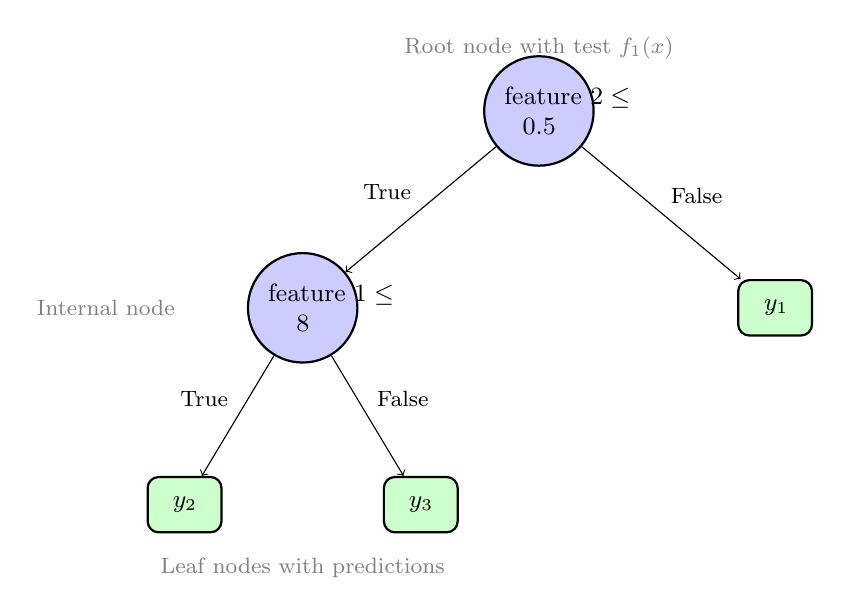
\begin{tikzpicture}[
        scale=1.0,
        decision/.style={circle, draw, thick, fill=blue!20, text width=2.5em, text centered, minimum height=2.5em, font=\small},
        leaf/.style={rectangle, draw, thick, fill=green!20, text width=2em, text centered, rounded corners, minimum height=2em, font=\small},
        edge_label/.style={font=\footnotesize, midway}
    ]
        % Root decision node
        \node[decision] (root) at (0,0) {$\text{feature 2}\leq 0.5$};
        
        % Second level nodes
        \node[decision] (left_decision) at (-3, -2.5) {$\text{feature 1}\leq 8$};
        \node[leaf] (right_leaf) at (3, -2.5) {$y_1$};
        
        % Third level nodes (leaves)
        \node[leaf] (left_left) at (-4.5, -5) {$y_2$};
        \node[leaf] (left_right) at (-1.5, -5) {$y_3$};
        
        % Connections with labels
        \draw[->] (root) -- (left_decision) node[edge_label, above left] {True};
        \draw[->] (root) -- (right_leaf) node[edge_label, above right] {False};
        \draw[->] (left_decision) -- (left_left) node[edge_label, above left] {True};
        \draw[->] (left_decision) -- (left_right) node[edge_label, above right] {False};
        
        % Add labels for components
        \node[font=\footnotesize, text=gray] at (0, 0.8) {Root node with test $f_1(x)$};
        \node[font=\footnotesize, text=gray] at (-5.5, -2.5) {Internal node};
        \node[font=\footnotesize, text=gray] at (-3, -5.8) {Leaf nodes with predictions};
        
    \end{tikzpicture}
    \caption{A generic depth 2 decision tree with 2 nodes and 3 leaves. Edges represent the outcomes of the tests in each internal nodes(True/False), and leaf nodes contain predictions $y_l \in \mathcal{Y}$. For any input $x_i$, the tree defines a unique path from root to leaf.}
    \label{fig:dt}
\end{figure}

\section{How to learn decision trees?}\label{sec:sl}
Training decision trees to optimize the supervised learning objective~\ref{def:sl} is well studied.

\begin{definition}[Supervised learning objective for classification or regression]\label{def:sl}
    Assume that we have access to a set of $N$ examples denoted $\mathcal{E} = {\{(x_i, y_i)\}}_{i=1}^N$. Each datum $x_i$ is described by a set of $p$ features. $y_i \in {\mathcal Y}$ is the label associated with $x_i$.
    For a classification task $\mathcal{Y}=\{1,\ldots,K\}$ and for a regression task $\mathcal{Y}\subseteq \mathbb{R}$.
    The goal of supervised learning for classification (or regression) tasks is to find a classifier (or regressor) $f:X \rightarrow  y$ that minimizes the following objective:
    \begin{align}
        \mathcal{L}_{\alpha}(f) = \frac{1}{N}\overset{N}{\underset{i=1}{\sum}}{l}(y_i, f(x_i)) + \alpha C(f),
        \label{eq:suplearning}
    \end{align}
    where $f$ is a model in a particular model class, e.g. the set of neural networks with relu activations or decision trees with depth at most 4, and where $C: \mathcal{F} \rightarrow \mathbb{R}$ is a regularization penalty.
    \end{definition}

The Classification and Regression Trees (CART) algorithm \cite{breiman1984classification} (algorithm~\ref{alg:cart}), developed by Leo Breiman and colleagues, is one of the most widely used method for learning decision trees from supervised data.
CART builds binary decision trees through a greedy, top-down approach that recursively partitions the feature space. 
At each internal node, the algorithm selects the feature and threshold that best split the data according to a purity criterion such as the Gini impurity for classification or mean squared error for regression.
CART uses threshold-based tests of the form $\mathbb{I}[x[\text{feature}] \leq \text{threshold}]$, where $\mathbb{I}[\cdot]$ is the indicator function. 
The key idea is to find splits that maximize the homogeneity of the resulting subsets. 
We use CART as well as other decision tree algorithms in this manuscript.

In particular, in the second part we will challenge decision tree algorithms that perform better than CART for the supervised learning objective.
In the first and third parts, we study CART in conjunction with reinforcement learning as a means to obtain decision trees for sequential decision making.

In the next few sections we present the material related to sequential decision making.

% \begin{figure}
%     \centering
%     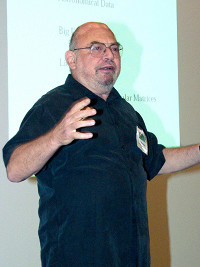
\includegraphics[width=0.3\textwidth]{images/images_intro/Leo_Breiman.jpg}
%     \caption{The american statistician Leo Breiman (1928-2005) author of \textit{Classification and Regression Trees} (1984)}
%     \label{fig:leo-breiman}
% \end{figure}

\RestyleAlgo{ruled}
\SetKwComment{Comment}{}{}
\begin{algorithm}
    \KwData{Training data $\mathcal{E} = \{(x_i, y_i)\}_{i=1}^N$ where $x_i \in \mathcal{X} \subseteq \mathbb{R}^p$ and $y_i \in \mathcal{Y} = \{1, \ldots, K\}$}
    \KwResult{Decision tree $T$}
    
    \SetKwProg{Fn}{Function}{:}{}
    \SetKwFunction{BuildTree}{BuildTree}
    \SetKwFunction{BestSplit}{BestSplit}
    \SetKwFunction{Gini}{Gini}
    \SetKwFunction{MajorityClass}{MajorityClass}
    
    \Fn{\BuildTree{$\mathcal{E}$}}{
        \If{stopping criterion met}{
            \Return leaf node with prediction $y_l \leftarrow$ MajorityClass$(\{y_i\}_{i=1}^N)$
        }
        
        $(feature, threshold) \leftarrow$ BestSplit$(\mathcal{E})$ \\
        
        \If{no valid split found}{
            \Return leaf node with prediction $y_l \leftarrow$ MajorityClass$(\{y_i\}_{i=1}^N)$
        }
        
        Split data: $\mathcal{E}_{left} = \{(x_i, y_i) \in \mathcal{E} : x_i[feature] \leq threshold\}$ \\
        \hspace{2.5cm} $\mathcal{E}_{right} = \{(x_i, y_i) \in \mathcal{E} : x_i[feature] > threshold\}$ \\
        
        $left\_child \leftarrow$ BuildTree$(\mathcal{E}_{left})$ \\
        $right\_child \leftarrow$ BuildTree$(\mathcal{E}_{right})$ \\
        
        \Return internal node with test function $f_v(x) = \mathbb{I}[x[feature] \leq threshold]$ and children $(left\_child, right\_child)$
    }
    
    \Fn{\BestSplit{$\mathcal{E}$}}{
        $best\_gain \leftarrow 0$ \\
        $best\_feature \leftarrow None$ \\
        $best\_threshold \leftarrow None$ \\
        
        \For{each feature $f \in \{1, \ldots, p\}$}{
            \For{each unique value $v$ in $\{x_i[f] : (x_i, y_i) \in \mathcal{E}\}$}{
                $\mathcal{Y}_{left} \leftarrow \{y_i : (x_i, y_i) \in \mathcal{E}, x_i[f] \leq v\}$ \\
                $\mathcal{Y}_{right} \leftarrow \{y_i : (x_i, y_i) \in \mathcal{E}, x_i[f] > v\}$ \\
                
                $gain \leftarrow$ Gini$(\{y_i\}_{i=1}^N) - \frac{|\mathcal{Y}_{left}|}{N}$Gini$(\mathcal{Y}_{left}) - \frac{|\mathcal{Y}_{right}|}{N}$Gini$(\mathcal{Y}_{right})$ \\
                
                \If{$gain > best\_gain$}{
                    $best\_gain \leftarrow gain$ \\
                    $best\_feature \leftarrow f$ \\
                    $best\_threshold \leftarrow v$ \\
                }
            }
        }
        \Return $(best\_feature, best\_threshold)$
    }
    
    \Fn{\Gini{$\mathcal{Y}$}}{
        \Return $1 - \sum_{k=1}^K \left(\frac{|\{y_i \in \mathcal{Y} : y_i = k\}|}{|\mathcal{Y}|}\right)^2$ \Comment{// Gini impurity}
    }
    
    \Return BuildTree$(\mathcal{E})$
    \caption{CART for decision tree induction to optimize the supervised learning objective~\ref{def:sl}}\label{alg:cart}
\end{algorithm}

\section{Markov decision processes and problems}
\begin{figure}
    \centering
    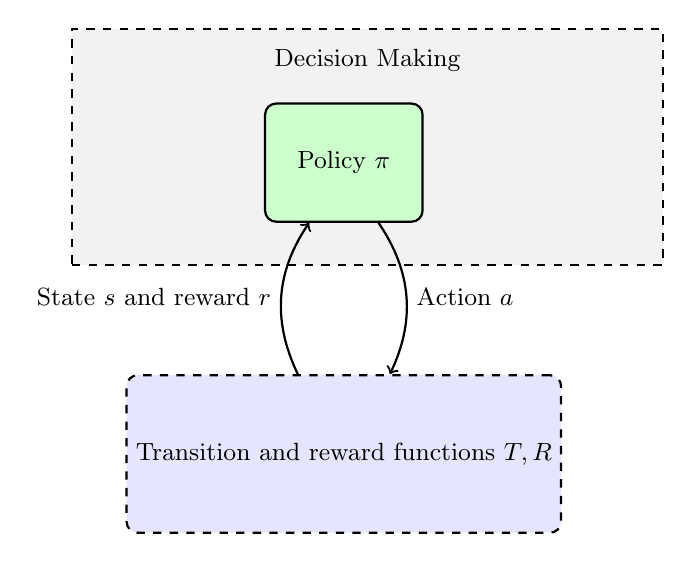
\begin{tikzpicture}[
        node distance=2.5cm,
        auto,
        thick,
        state/.style={circle, draw, fill=blue!20, minimum size=1.5cm, text centered},
        environment/.style={rectangle, draw, dashed, fill=blue!10, rounded corners, minimum width=4cm, minimum height=2cm, text centered},
        agent/.style={rectangle, draw, fill=orange!20, rounded corners, minimum width=2cm, minimum height=1.5cm, text centered},
        robot/.style={rectangle, draw, fill=green!20, rounded corners, minimum width=2cm, minimum height=1.5cm, text centered},
        decision_box/.style={rectangle, draw, dashed, fill=gray!10, minimum width=7.5cm, minimum height=3cm, text centered},
        arrow/.style={->, thick, bend left=15},
        arrow_decision/.style={->, dashed, bend left=15}
    ]
        
        % Decision Making Box
        \node[decision_box] (decision_box) at (0.3,3.4) {};
        \node at (0.3,4.5) {\small{Decision Making}};
        
        % Robot (AI)
        \node[robot] (robot) at (0,3.2) {\small{Policy $\pi$}};
        
        
        % Environment (Patient)
        \node[environment] (environment) at (0,-0.5) {\small{Transition and reward functions $T, R$}};
        
        % Arrows
        \draw[arrow] (environment) to[bend left=30] node[left] {\small{State $s$ and reward $r$}} (robot);
        \draw[arrow] (robot) to[bend left=30] node[right] {\small{Action $a$}} (environment);
        
    \end{tikzpicture}
    \caption{Markov decision process}
    \label{fig:MDP}
\end{figure}

Markov decision processes (MDPs) were first introduced in the 1950s by Richard Bellman~\cite{Bellman}.
Informally, an MDP models how an agent acts over time to achieve a goal. 
At every time step, the agent observes its current state (e.g., patient weight and tumor size) and takes an action (e.g., administers a certain amount of chemotherapy).
The agent receives a reward that helps evaluate the quality of the action with respect to the goal (e.g., tumor size decreases when the objective is to cure cancer).
Finally, the agent transitions to a new state (e.g., the updated patient state) and repeats this process over time. 
Following Martin L. Puterman's book on MDPs\cite{puterman}, we formally define:
\begin{definition}[Markov decision process]\label{def:mdp} An MDP is a tuple $\mathcal{M} = \langle S, A, R, T, T_0 \rangle$ where:
\begin{itemize}
\item $S$ is a finite set of states representing all possible configurations of the environment.
\item $A$ is a finite set of actions available to the agent.
\item $R: S \times A \rightarrow \mathbb{R}$ is the reward function that assigns a real-valued reward to each state-action pair.
\item $T: S \times A \rightarrow \Delta(S)$ is the transition function that maps state-action pairs to probability distributions over next states, where $\Delta(S)$ denotes a probability distribution over $S$.
\item $T_0 \in \Delta(S)$ is the initial distribution over states.
\end{itemize}
\end{definition}

Informally, we would like to act in an MDP such that we obtain as much reward as possible over time.
For example, in cancer treatment, the best outcome is to eliminate the patient's tumor as quickly as possible.
We can formally define this objective, that we call the reinforcement learning objective, as follows:

\begin{definition}[Reinforcement learning objective]\label{def:mdp-obj} Given an MDP $\mathcal{M}=\langle S, A, R, T, T_0 \rangle$ (~\ref{def:mdp}), the objective of a model, aslo known as a policy $\pi: S \rightarrow A$ is to maximize the expected discounted sum of rewards:
$$J(\pi) = \mathbb{E}\left[\sum_{t=0}^{\infty} \gamma^t R(s_t, a_t) \mid s_0 \sim T_0, a_t = \pi(s_t), s_{t+1} \sim T(s_t, a_t)\right]$$
where $\gamma \in (0,1]$ is the discount factor that controls the trade-off between immediate and future rewards.
\end{definition}

Hence, algorithms presented in this manuscript aim to find policies that maximize this RL objective, i.e., an optimal policy: $\pi^\star \in\underset{\pi}{\operatorname{argmax}}J(\pi)$.

\subsection{Example: a grid world MDP}
\begin{figure}
    \centering
    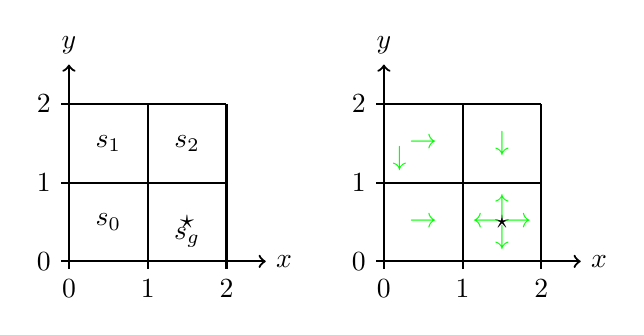
\begin{tikzpicture}
        \tikzstyle{grid}=[draw, thick, fill=gray!10]
        
        % Draw grid
        \draw[grid] (0,0) grid (2,2);
        
        % Add axes
        \draw[thick, ->] (0,0) -- (2.5,0) node[right] {$x$};
        \draw[thick, ->] (0,0) -- (0,2.5) node[above] {$y$};
        
        % Add tick marks and labels
        \foreach \x in {0,1,2} {
            \draw[thick] (\x,0) -- (\x,-0.1) node[below] {$\x$};
        }
        \foreach \y in {0,1,2} {
            \draw[thick] (0,\y) -- (-0.1,\y) node[left] {$\y$};
        }
        
        % Add state labels clockwise from bottom left
        \node at (0.5,0.5) {$s_0$};
        \node at (1.5,0.5) {$\star$};
        \node at (1.5,0.3) {$s_g$};
        \node at (1.5,1.5) {$s_2$};
        \node at (0.5,1.5) {$s_1$};


        % Draw grid
        \draw[grid] (4,0) grid (6,2);
        
        % Add axes
        \draw[thick, ->] (4,0) -- (6.5,0) node[right] {$x$};
        \draw[thick, ->] (4,0) -- (4,2.5) node[above] {$y$};
        
        % Add tick marks and labels
        \draw[thick] (4,0) -- (4,-0.1) node[below] {$0$};
        \draw[thick] (5,0) -- (5,-0.1) node[below] {$1$};
        \draw[thick] (6,0) -- (6,-0.1) node[below] {$2$};
        

        \foreach \y in {0,1,2} {
            \draw[thick] (4,\y) -- (3.9,\y) node[left] {$\y$};
        }
        
        % Add state labels clockwise from bottom left
        \node at (4.5,0.5) {{\color{green} $\rightarrow$}};
        \node at (5.5,0.5) {$\star$};
        \node at (5.5,0.7) {{\color{green} $\uparrow$}};
        \node at (5.5,0.3) {{\color{green} $\downarrow$}};
        \node at (5.7,0.5) {{\color{green} $\rightarrow$}};
        \node at (5.3,0.5) {{\color{green} $\leftarrow$}};
        \node at (5.5,1.5) {{\color{green} $\downarrow$}};
        \node at (4.2,1.3) {{\color{green} $\downarrow$}};
        \node at (4.5,1.5) {{\color{green} $\rightarrow$}};
    \end{tikzpicture}
    \caption{A grid world MDP (left) and optimal actions w.r.t. the objective~\ref{def:mdp-obj} (right).}\label{example:grid}
    \end{figure}

In figure~\ref{example:grid}, we present a very simple MDP(~\ref{def:mdp}).
This MDP is essentially a grid where the starting state is chosen at random and the goal is to reach the bottom-right cell as fast as possible in order to maximize the objective~\ref{def:mdp-obj}.
The state space is discrete with state labels representing 2D-coordinates.
The actions are to move up, left, right, or down. The MDP transitions to the resulting cell. 
Only the bottom-right cell gives reward 1 and is an absorbing state, i.e., once in the state, the MDP stays in this state forever.
The optimal actions that get to the goal as fast as possible in every state (cell) are presented in green.

Next we present the tools to find solutions to MDPs and retrieve such optimal policies.

\section{Exact solutions for Markov decision problems}\label{sec:values}
We begin with the planning setting in which the model is known. Leveraging the Markov property, dynamic programming computes optimal value functions and extracts an optimal policy; we define $V$ and $Q$ and then present Value Iteration.
It is possible to compute the exact optimal policy $\pi^\star$ using dynamic programming\cite{Bellman}.
Indeed, one can leverage the Markov property to find for all states the best action to take based on the reward of upcoming states.
\begin{definition}[Value of a state]\label{def:vs} 
    The value of a state $s\in S$ under policy $\pi$ is the expected discounted sum of rewards starting from state $s$ and following policy $\pi$:
    $$V^\pi(s) = \mathbb{E}\left[\sum_{t=0}^{\infty} \gamma^t R(s_t, a_t) \mid s_0 = s, a_t = \pi(s_t), s_{t+1} \sim T(s_t, a_t)\right]$$
    Applying the Markov property gives a recursive definition of the value of $s$ under policy $\pi$:
    $$V^\pi(s) = R(s,\pi(s)) + \gamma \sum_{s' \in S} T(s,\pi(s),s')\,V^\pi(s')$$
    where $T(s,a,s')$ is the probability of transitioning to state $s'$ when taking action $a$ in state $s$.
\end{definition}
\begin{definition}[Optimal value of a state] The optimal value of a state $s\in S$, $V^\star(s)$, is the value of state $s$ when following the optimal policy $\pi^{\star}$ (the policy that maximizes the RL objective (\ref{def:mdp-obj})).
    $$V^{\star}(s) = V^{\pi^{\star}}(s)$$
\end{definition}
\begin{definition}[Optimal value of a state–action pair] The optimal value of a state–action pair $(s,a)\in S\times A$, $Q^\star(s,a)$, is the value when taking action $a$ in state $s$ and then following the optimal policy.
    $$Q^{\star}(s,a) = R(s, a) + \gamma\sum_{s'\in S} T(s,a,s')\,V^{\star}(s')$$
\end{definition}

Hence, we can use the definition of the value function to re-write the RL objective (\ref{def:mdp-obj}): $\pi^{\star} = \underset{\pi}{\operatorname{argmax}}\mathbb{E}\left[V^{\pi}(s_0)|s_0\sim T_0 \right]$.
The well-known Value Iteration algorithm~\ref{alg:value-iteration} solves this problem exactly. 

\RestyleAlgo{ruled}
\SetKwComment{Comment}{}{}
\begin{algorithm}
    \KwData{MDP $\mathcal{M} = \langle S, A, R, T, T_0 \rangle$, convergence threshold $\theta$}
    \KwResult{Optimal policy $\pi^*$}
    Initialize $V(s) = 0$ for all $s \in S$ \\
    \Repeat{$\Delta < \theta$}{
        $\Delta \leftarrow 0$ \\
        \For{each state $s \in S$}{
            $v \leftarrow V(s)$ \\
            $V(s) \leftarrow \max_a \left[ R(s,a) + \gamma \sum_{s' \in S} T(s,a,s') V(s') \right]$ \Comment{// Bellman optimality update}
            $\Delta \leftarrow \max(\Delta, |v - V(s)|)$
        }
    }
    \For{each state $s \in S$}{
        $\pi^*(s) \leftarrow \operatorname{argmax}_a \left[ R(s,a) + \gamma \sum_{s' \in S} T(s,a,s') V(s') \right]$ \Comment{// Extract optimal policy}
    }
    \caption{Value Iteration}\label{alg:value-iteration}
\end{algorithm}

More realistically, neither the transition kernel $T$ nor the reward function $R$ of the MDP are known; e.g., the doctor cannot \textbf{know} how the tumor and the patient's health will change after a dose of chemotherapy, but can only \textbf{observe} the change.
This distinction in available information parallels the distinction between dynamic programming and reinforcement learning (RL), described next. 

\section{Reinforcement learning of approximate solutions to MDPs}\label{sec:rl}
When the dynamics and rewards are unknown, we turn to model-free RL. 
% \begin{figure}
%     \centering
%     \begin{subfigure}[b]{0.22\textwidth}
%         \centering
%         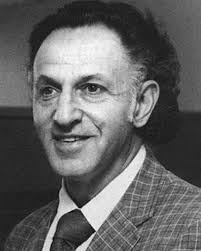
\includegraphics[width=0.7\textwidth]{images/images_intro/bellman.jpeg}
%         \caption{R. Bellman}
%     \end{subfigure}
%     \hfill
%     \begin{subfigure}[b]{0.22\textwidth}
%         \centering
%         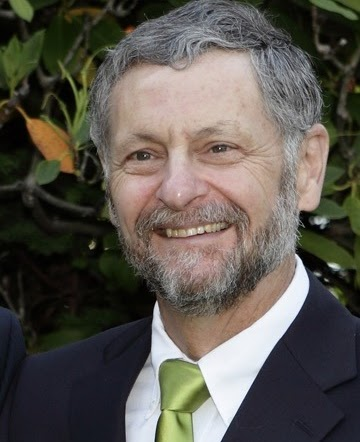
\includegraphics[width=0.7\textwidth]{images/images_intro/puterman.jpg}
%         \caption{M.L. Puterman}
%     \end{subfigure}
%     \hfill
%     \begin{subfigure}[b]{0.22\textwidth}
%         \centering
%         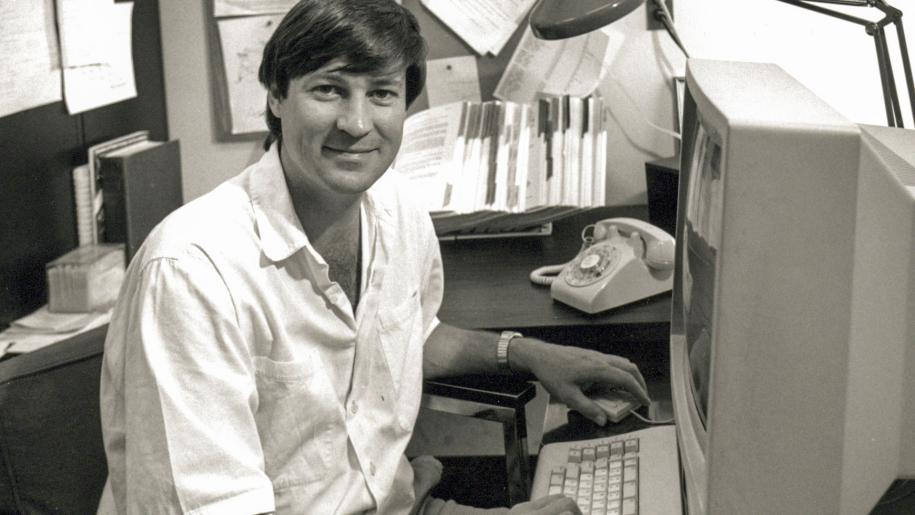
\includegraphics[width=1.2\textwidth]{images/images_intro/Barto_1982_umass_amherst.jpg}
%         \caption{A. Barto}
%     \end{subfigure}
%     \hfill
%     \begin{subfigure}[b]{0.22\textwidth}
%         \centering
%         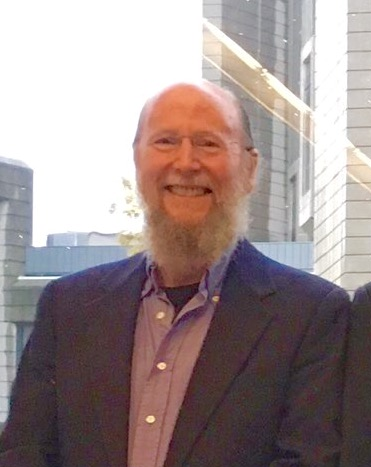
\includegraphics[width=0.67\textwidth]{images/images_intro/sutton.jpg}
%         \caption{R. Sutton}
%     \end{subfigure}
%        \caption{The godfathers of sequential decision making. Andrew Barto and Richard Sutton are the ACM Turing Prize 2024 laureate and share an advisor advisee relationship.}
%        \label{fig:rl-pioneers}
% \end{figure}

Reinforcement learning algorithms popularized by Richard Sutton~\cite{sutton} don't \textbf{compute} an optimal policy but rather \textbf{learn} an approximate one based on sequences of observations ${(s_t, a_t, r_t, s_{t+1})}_t$.
RL algorithms usually fall into two categories: value-based and policy search~\cite{pg_sutton}.
Examples of these approaches are shown in algorithms~\ref{alg:qlearning},~\ref{alg:sarsa} and~\ref{alg:reinforce}.
Q-learning and Sarsa compute an approximation of $Q^{\star}$ using temporal difference learning. Q-learning is \textit{off policy}, it collects new transisitions with a random policy, e.g. epsilon-greedy, while Sarsa is on policy, it collects new transitions greedily w.r.t. the current q-values estimates.
Policy gradient algorithms leverages the policy gradient theorem to approximate $\pi^{\star}$.
The goal of an RL algorithm (also called agent) is to learn a policy that solves a Markov decision problem(~\ref{def:mdp-obj}) without access to transitions and rewards from the MDP.
From now on, we refer to~\ref{def:mdp-obj} as the RL objective.

Q-learning, Sarsa, and Policy gradients are known to converge to the optimal value or (locally) optimal policy under some conditions.
The books from Puterman~\cite{puterman}, or Sutton and Barto~\cite{sutton}, offer a great overview of MDPs and algorithms to solve them.
There are many other ways to learn policies such as simple random search~\cite{random-search} or model-based reinforcement learning~\cite{dyna}. 
However, not many algorithms consider the learning of policies that can be easily understood by humans which we discuss next and that is the core of this manuscript.

\RestyleAlgo{ruled}
\SetKwComment{Comment}{}{}
\begin{algorithm}
    \KwData{MDP $\mathcal{M} = \langle S, A, R, T, T_0 \rangle$, learning rate $\alpha$, exploration rate $\epsilon$}
    \KwResult{Policy $\pi$}
    Initialize $Q(s,a) = 0$ for all $s \in S, a \in A$ \\
    Initialize state $s_0 \sim T_0$ \\
    \For{each step $t$}{
        Choose action $a_t$ using $\epsilon$-greedy: $a_t = \operatorname{argmax}_a Q(s_t,a)$ with prob. $1-\epsilon$ \\
        Take action $a_t$, observe $r_t = R(s_t,a_t)$ and $s_{t+1} \sim T(s_t,a_t)$ \\
        $Q(s_t,a_t) \leftarrow Q(s_t,a_t) + \alpha[r_t + \gamma \max_{a'} Q(s_{t+1},a') - Q(s_t,a_t)]$ \\
        $s_t \leftarrow s_{t+1}$ \\
    }
    $\pi(s) = \operatorname{argmax}_a Q(s,a)$ \Comment{// Extract greedy policy}
    \caption{Q-Learning}\label{alg:qlearning}
\end{algorithm}


\RestyleAlgo{ruled}
\SetKwComment{Comment}{}{}
\begin{algorithm}
    \KwData{MDP $\mathcal{M} = \langle S, A, R, T, T_0 \rangle$, learning rate $\alpha$, exploration rate $\epsilon$}
    \KwResult{Policy $\pi$}
    Initialize $Q(s,a) = 0$ for all $s \in S, a \in A$ \\
    Initialize state $s_0 \sim T_0$ \\
    Choose action $a_0$ using $\epsilon$-greedy: $a_0 = \operatorname{argmax}_a Q(s_0,a)$ with prob. $1-\epsilon$ \\
    \For{each step $t$}{
        Take action $a_t$, observe $r_t = R(s_t,a_t)$ and $s_{t+1} \sim T(s_t,a_t)$ \\
        Choose action $a_{t+1}$ using $\epsilon$-greedy: $a_{t+1} = \operatorname{argmax}_a Q(s_{t+1},a)$ with prob. $1-\epsilon$ \\
        $Q(s_t,a_t) \leftarrow Q(s_t,a_t) + \alpha[r_t + \gamma Q(s_{t+1},a_{t+1}) - Q(s_t,a_t)]$ \\
        $s_t \leftarrow s_{t+1}$ \\
        $a_t \leftarrow a_{t+1}$ \\
    }
    $\pi(s) = \operatorname{argmax}_a Q(s,a)$ \Comment{// Extract greedy policy}
    \caption{Sarsa}\label{alg:sarsa}
\end{algorithm}


\RestyleAlgo{ruled}
\SetKwComment{Comment}{}{}
\begin{algorithm}
    \KwData{MDP $\mathcal{M} = \langle S, A, R, T, T_0 \rangle$, learning rate $\alpha$, policy parameters $\theta$}
    \KwResult{Policy $\pi_\theta$}
    Initialize policy parameters $\theta$ \\
    \For{each episode}{
        Generate trajectory $\tau = (s_0, a_0, r_0, s_1, a_1, r_1, \ldots)$ following $\pi_\theta$ \\
        \For{each time step $t$ in trajectory}{
            $G_t \leftarrow \sum_{k=t}^{T} \gamma^{k-t} r_k$ \Comment{// Compute return}
            $\theta \leftarrow \theta + \alpha G_t \nabla_\theta \log \pi_\theta(a_t|s_t)$ \Comment{// Policy gradient update}
        }
    }
    \caption{Policy Gradient RL (REINFORCE)}\label{alg:reinforce}
\end{algorithm}


\section{Deep reinforcement learning for large or continuous state spaces}\label{sec:drl}

Reinforcement learning has also been successfully combined with function approximations \cite{td-gammon} to solve MDPs with large discrete state spaces or continuous state spaces ($S \subset \mathbb{R^p}$).
Such continuous states MDP can be formalized as factored MDPs\cite{fmdp}:

\begin{definition}[Factored Markov decision process]\label{def:fmdp} A factored MDP is an MDP\ref{def:mdp} where the state space is a hyperrectangle: $S\subseteq \mathbb{R}^p$.
\end{definition}

From now on, all the MDPs we study in the this manuscript are factored unless stated otherwise. 
We also consider that the Example MDP(\ref{example:grid}) is continuous with two state dimensions.
In the rest of this manuscript, unless stated otherwise, we write $\boldsymbol{s}$ a state vector in a continuous space.
Note that discrete states MDP can be encoded into factored MDP by one-hot encoding individual states.

Deep Q-Networks (DQN)~\cite{dqn}, described in algorithm~\ref{alg:dqn} was a breakthrough in modern reinforcement learning.
Authors successfully extended the Q-learning (algorithm~\ref{alg:qlearning}) to the function approximation setting by introduction target networks to mitigate distributional shift in the td error and replay buffer to increase sample efficiency.
DQN achieved super-human performance on a set of Atari games.

Proximal Policy Optimization (PPO)~\cite{ppo}, described in algorithm~\ref{alg:ppo}, is an actor-critic algorithm\cite{pg_sutton} optimizing neural network policies. 
Actor-critic algorithms are instances of policy gradient algorithms where the cumulative discounted rewards--the returns--are also estimated with a neural network. 
Actor-critic are not as simple efficient as DQN but is known to work well in a variety of domains including robot control in simulation among others.

\begin{algorithm}
    \KwData{MDP $\mathcal{M} = \langle S, A, R, T, T_0 \rangle$, learning rate $\alpha$, exploration rate $\epsilon$, Q-network parameters $\theta$, update frequency $C$}
    \KwResult{Policy $\pi$}
    Initialize Q-network parameters $\theta$ and target network parameters $\theta^- = \theta$ \\
    Initialize replay buffer $\mathcal{B} = \emptyset$ \\
    \For{each episode}{
        Initialize state $s_0 \sim T_0$ \\
        \For{each step $t$}{
            Choose action $a_t$ using $\epsilon$-greedy: $a_t = \operatorname{argmax}_a Q_\theta(\boldsymbol{s}_t,a)$ with prob. $1-\epsilon$ \\
            Take action $a_t$, observe $r_t = R(s_t,a_t)$ and $\boldsymbol{s}_{t+1} \sim T(\boldsymbol{s}_t,a_t)$ \\
            Store transition $(\boldsymbol{s}_t, a_t, r_t, \boldsymbol{s}_{t+1})$ in $\mathcal{B}$ \\
            Sample random batch $(\boldsymbol{s}_i, a_i, r_i, \boldsymbol{s}_{i+1}) \sim \mathcal{B}$ \\
            $y_i = r_i + \gamma \max_{a'} Q_{\theta^-}(\boldsymbol{s}_{i+1}, a')$ \Comment{// Compute target}
            $\theta \leftarrow \theta - \alpha \nabla_\theta (Q_\theta(\boldsymbol{s}_i, a_i) - y_i)^2$ \Comment{// Update Q-network}
            \If{$t \bmod C = 0$}{
                $\theta^- \leftarrow \theta$ \Comment{// Update target network}
            }
            $\boldsymbol{s}_t \leftarrow \boldsymbol{s}_{t+1}$ \\
        }
    }
    $\pi(\boldsymbol{s}) = \operatorname{argmax}_a Q_\theta(\boldsymbol{s},a)$ \Comment{// Extract greedy policy}
    \caption{Deep Q-Network (DQN)}\label{alg:dqn}
\end{algorithm}


\begin{algorithm}
    \KwData{MDP $\mathcal{M} = \langle S, A, R, T, T_0 \rangle$, learning rate $\alpha$, policy parameters $\theta$, clipping parameter $\epsilon$, value function parameters $\phi$}
    \KwResult{Policy $\pi_\theta$}
    Initialize policy parameters $\theta$ and value function parameters $\phi$ \\
    \For{each episode}{
        Generate trajectory $\tau = (\boldsymbol{s}_0, a_0, r_0, \boldsymbol{s}_1, a_1, r_1, \ldots)$ following $\pi_\theta$ \\
        \For{each time step $t$ in trajectory}{
            $G_t \leftarrow \sum_{k=t}^{T} \gamma^{k-t} r_k$ \Comment{// Compute return}
            $A_t \leftarrow G_t - V_\phi(\boldsymbol{s}_t)$ \Comment{// Compute advantage}
            $r_t(\theta) \leftarrow \frac{\pi_\theta(a_t|\boldsymbol{s}_t)}{\pi_{\theta_{old}}(a_t|\boldsymbol{s}_t)}$ \Comment{// Compute probability ratio}
            $L^{CLIP}_t \leftarrow \min(r_t(\theta) A_t, \text{clip}(r_t(\theta), 1-\epsilon, 1+\epsilon) A_t)$ \Comment{// Clipped objective}
            $\theta \leftarrow \theta + \alpha \nabla_\theta L^{CLIP}_t$ \Comment{// Policy update}
            $\phi \leftarrow \phi + \alpha \nabla_\phi (G_t - V_\phi(\boldsymbol{s}_t))^2$ \Comment{// Value function update}
        }
        $\theta_{old} \leftarrow \theta$ \Comment{// Update old policy}
    }
    \caption{Proximal Policy Optimization (PPO)}\label{alg:ppo}
\end{algorithm}
In this manuscript we study those two deep reinforcement learning algorithms for various problems.

\section{Imitation learning: a baseline (indirect) interpretable reinforcement learning method}\label{sec:imit}

Unlike PPO or DQN for neural networks, there does not exist an algorithm that trains decision tree policies to optimize the RL objective (\ref{def:mdp-obj}).
In fact, we will show in the first part of the manuscript that training decision trees that optimize the RL objective is very difficult.

Hence, many interpretable reinforcement learning approaches first train a neural network policy with, e.g., DQN or PPO to optimize the RL objective (\ref{def:mdp-obj}), and then fit, e.g., a decision tree using CART (algorithm\ref{alg:cart}) to optimize the supervised learning objective (\ref{def:sl}) with the neural policy's actions as targets.
This approach is known as imitation learning and is essentially training a policy to optimize the objective:

\begin{definition}[Imitation learning objective]\label{def:il}
Given an MDP $\mathcal{M}$ (\ref{def:mdp}) expert policy $\pi^*$ and a policy class $\Pi$, the imitation learning objective is to find a policy $\hat{pi} \in \Pi$ that minimizes the expected action disagreement with the expert:
\begin{equation}
IL(\pi) &=  \mathbb{E}_{\boldsymbol{s} \sim \rho(\boldsymbol{s})} \left[ \mathcal{L}(\pi(\boldsymbol{s}), \pi^*(\boldsymbol{s})) \right]
\end{equation}
where $\rho(\boldsymbol{s})$ is the state distribution in $\mathcal{M}$ induced by the expert policy and $\mathcal{L}$ is a loss function measuring the disagreement between the learned policy's action $\pi(s)$ and the expert's action $\pi^*(s)$.
\end{definition}

There are two main imitation learning methods used for interpretable reinforcement learning.
Dagger (\cite{PIRL}; algorithm~\ref{alg:dagger}) is a straightforward way to fit a decision tree policy to optimize the imitation learning objective\ref{def:il}.
VIPER (\cite{viper}; algorithm~\ref{alg:viper}) was designed specifically for interpretable reinforcement learning.
VIPER reweights the transitions collected by the neural network expert by a function of the state–action value\ref{sec:values}.
The authors of VIPER showed that decision tree policies fitted with VIPER tend to have the same RL objective value as Dagger trees while being more interpretable (shallower or with fewer nodes) and sometimes outperform Dagger trees.
Dagger and VIPER are two strong baselines for decision tree learning in MDPs, but they optimize a surrogate objective only, even though in practice the resulting decision tree policies often achieve high RL objective value.

We use the two algorithms extensively throughout the manuscript.

Next we show how to learn a decision tree policy for the Example MDP \ref{example:grid}.
\begin{algorithm}
    \caption{Dagger}\label{alg:dagger}
    \KwIn{Expert policy $\pi^*$, MDP $M$, policy class $\Pi$}
    \KwOut{Fitted student policy $\hat{\pi}_i$}
    
    % Initialize empty dataset and initial policy
    Initialize dataset $\mathcal{D} \gets \emptyset$\;
    Initialize $\hat{\pi}_1$ arbitrarily from $\Pi$\;
    
    \For{$i \gets 1$ \KwTo $N$}{
        % Create mixed policy using expert and current policy
        \lIf{i = 1}{
        $\hat{\pi} \gets \pi^*$\
        }
          \lElse{
            $\pi_i \gets \hat{\pi}_i$
          } \label{alg:expert-or-student}
        % Collect data using mixed policy
        Sample transitions from $M$ using $\hat{\pi}$\;
        % Get expert actions for visited states
        Collect dataset $\mathcal{D}_i \gets \{ (\boldsymbol{s}, \pi^*(\boldsymbol{s})) \}$ of states visited by $\hat{\pi}$\;
        
        % Aggregate datasets
        $\mathcal{D} \gets \mathcal{D} \cup \mathcal{D}_i$\;
        
        % Train new policy
       Fit classifier/regressor $\hat{\pi}_{i+1}$ on $\mathcal{D}$\;\label{alg:fit}
    }
    \Return $\hat{\pi}$\;
    \end{algorithm}


    \begin{algorithm}
        \caption{VIPER}\label{alg:viper}
        \KwIn{Expert policy $\pi^*$, Expert Q-function $Q^*$, MDP $M$, policy class $\Pi$}
        \KwOut{Fitted student policy $\hat{\pi}_i$}
        
        % Initialize empty dataset and initial policy
        Initialize dataset $\mathcal{D} \gets \emptyset$\;
        Initialize $\hat{\pi}_1$ arbitrarily from $\Pi$\;
        
        \For{$i \gets 1$ \KwTo $N$}{
            % Create mixed policy using expert and current policy
            \lIf{i = 1}{
            $\hat{\pi} \gets \pi^*$\
            }
              \lElse{
                $\pi_i \gets \hat{\pi}_i$
              } \label{alg:expert-or-student}
            % Collect data using mixed policy
            Sample transitions from $M$ using $\hat{\pi}$\;
            % Get expert actions for visited states
            Weight each transition by $w(\boldsymbol{s}) \gets V^{\pi^*}(\boldsymbol{s}) - \min_a Q^{\pi^*}(\boldsymbol{s}, a)$\;
            Collect dataset $\mathcal{D}_i \gets \{ (\boldsymbol{s}, \pi^*(\boldsymbol{s}), w(\boldsymbol{s})) \}$ of states visited by $\hat{\pi}$\;            
            % Aggregate datasets
            $\mathcal{D} \gets \mathcal{D} \cup \mathcal{D}_i$\;
            
            % Train new policy
           Fit classifier/regressor $\hat{\pi}_{i+1}$ on the weighted dataset $\mathcal{D}$\;\label{alg:fit}
        }
        \Return $\hat{\pi}$\;
        \end{algorithm}

\section{Your first decision tree policy}\label{sec:limits-il}
Now the reader should know how to train decision tree classifiers or regressors for supervised learning using CART\ref{sec:sl}.
The reader should also know what an MDP is and how to compute or learn policies that optimize the RL objective \ref{def:mdp-obj} with (deep) reinforcement learning\ref{sec:drl}.
Finally, the reader should now know how to obtain a decision tree policy for an MDP through imitation learning by first using RL to get an expert policy and then fitting decision trees to optimize the supervised learning objective\ref{def:sl}, using the expert's actions as labels.
Note that, in theory, there is no guarantee that such decision tree policies also maximize the RL objective; they optimize only the imitation learning objective\ref{def:il}.

In this section we present the first decision tree policies of this manuscript obtained using Dagger or VIPER after learning an expert policy and expert Q-function for the grid world MDP \ref{example:grid} with Q-learning\ref{alg:qlearning}.
Recall the optimal policies for the grid world, taking the green actions in each state in figure\ref{example:grid}. 
Among the optimal policies, the ones that take action to go left or up in the goal state can be problematic for imitation learning algorithms.

Indeed, we know that for this grid world MDP there exists a decision tree policy that is optimal and very interpretable (depth-1): go right if the $x$-label of the state is greater than 1 and go left otherwise.
This tree takes exactly the same actions in the same states as some of the optimal policy from figure\ref{example:grid}.

In figure\ref{fig:trees-intro}, we present a depth-1 decision tree policy that is optimal w.r.t. the RL objective and a depth-1 tree that is sub-optimal.
Indeed, figure\ref{fig:objectives} shows that the optimal depth-1 tree achieves exactly the same RL objective value as the optimal policies from figure\ref{example:grid}, independently of the discount factor $\gamma$.

Now a fair question is: can Dagger or VIPER retrieve such an optimal depth-1 tree given access to an expert optimal policy from figure\ref{example:grid}?

We start by running the standard Q-learning algorithm as presented in algorithm\ref{alg:qlearning} with $\epsilon=0.3$, $\alpha=0.1$ over 10,000 time steps.
The careful reader might wonder how ties are broken in the $\operatorname{argmax}$ operation from algorithm\ref{alg:qlearning}.
While Sutton and Barto break ties by index value in their book\cite{sutton} (the greedy action is the $\operatorname{argmax}$ action with smallest index), we show that the choice of tie-breaking greatly influences the performance of subsequent imitation learning algorithms.
Indeed, depending on how actions are ordered in practice, Q-learning may be biased toward some optimal policies rather than others.
While this does not matter for one who just wants to find an optimal policy, in our example of finding the optimal depth-1 decision tree policy, it matters \textit{a lot}.

In the left plot of figure\ref{fig:ql-il}, we see that Q-learning, independently of how ties are broken, consistently converges to an optimal policy over 100 runs (random seeds).
However, in the right plot of figure\ref{fig:ql-il}, where we plot the proportion over 100 runs of optimal decision trees returned by Dagger or VIPER at different stages of Q-learning, we observe that imitating the optimal policy obtained by breaking ties at random consistently yields more optimal trees than breaking ties by indices.
What actually happens is that the most likely output of Q-learning when ties are broken by indices is the optimal policy that goes left in the goal state,
which cannot be perfectly represented by a depth-1 decision tree, because there are three different actions taken and a binary tree of depth $D=1$ can only map to $2^D=2$ labels.

Despite this negative result, we still find that VIPER almost always finds the optimal depth-1 decision tree policy in terms of the RL objective\ref{def:mdp-obj} when ties are broken at random.
Importantly, this sheds light on the sub-optimality of indirect imitation w.r.t the RL objective (~\ref{def:mdp-obj}) and motivates the study of direct approaches.
\begin{figure}
    \centering
    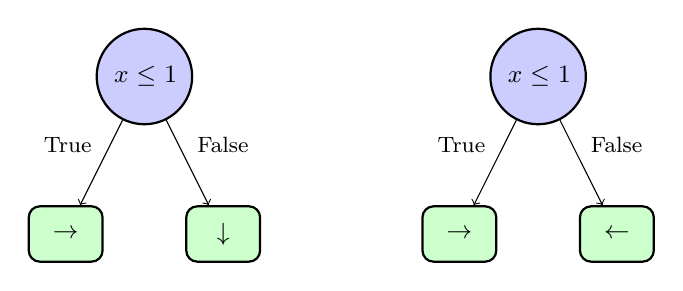
\begin{tikzpicture}[
        decision/.style={circle, draw, thick, fill=blue!20, text width=2.5em, text centered, minimum height=2.5em, font=\small},
        leaf/.style={rectangle, draw, thick, fill=green!20, text width=2em, text centered, rounded corners, minimum height=2em, font=\small},
        edge_label/.style={font=\footnotesize, midway}
    ]
        % Tree 4: if x <= 0.5 move right else move left
        \node[decision] (tree4_root) at (10,2) {$x \leq 1$};
        \node[leaf] (tree4_right) at (9,0) {$\rightarrow$};
        \node[leaf] (tree4_left) at (11,0) {$\leftarrow$};
        \draw[->] (tree4_root) -- (tree4_right) node[edge_label, above left] {True};
        \draw[->] (tree4_root) -- (tree4_left) node[edge_label, above right] {False};
        \tikzstyle{grid}=[draw, thick, fill=gray!10]


        % Tree 4: if x <= 0.5 move right else move left
        \node[decision] (tree5_root) at (5,2) {$x \leq 1$};
        \node[leaf] (tree5_right) at (4,0) {$\rightarrow$};
        \node[leaf] (tree5_left) at (6,0) {$\downarrow$};
        \draw[->] (tree5_root) -- (tree5_right) node[edge_label, above left] {True};
        \draw[->] (tree5_root) -- (tree5_left) node[edge_label, above right] {False};
        \tikzstyle{grid}=[draw, thick, fill=gray!10]

    \end{tikzpicture}
    \caption{Left, an optimal depth-1 decision tree policy. On the right, a sub-optimal depth-1 decision tree policy.}\label{fig:trees-intro}
    \end{figure}

\begin{figure}
    \centering
    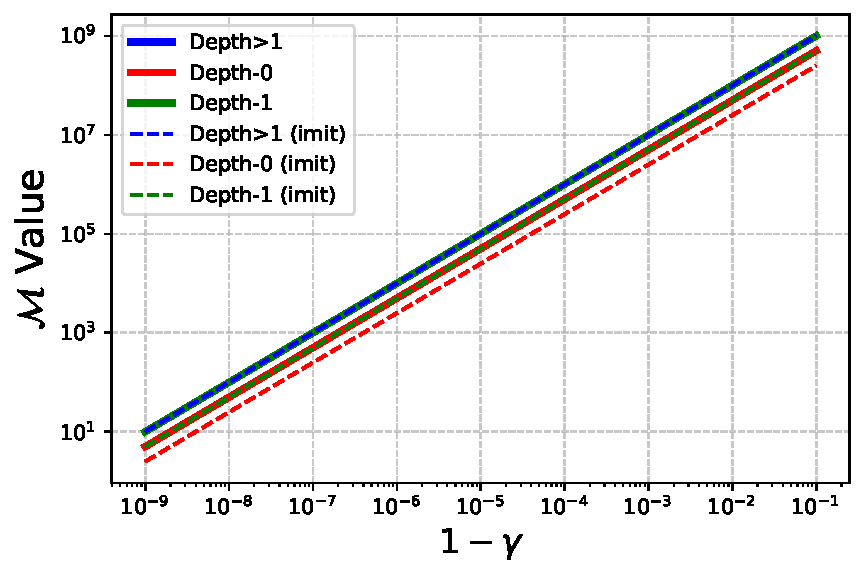
\includegraphics[width=0.4\textwidth]{images/images_part1/policy_values_comparison.pdf}
    \caption{The objective (\ref{def:mdp-obj}) values of the optimal policies from figure~\ref{example:grid} and of the decision tree policies from figure~\ref{fig:trees-intro}.}\label{fig:objectives}
\end{figure}

\begin{figure}
    \centering
    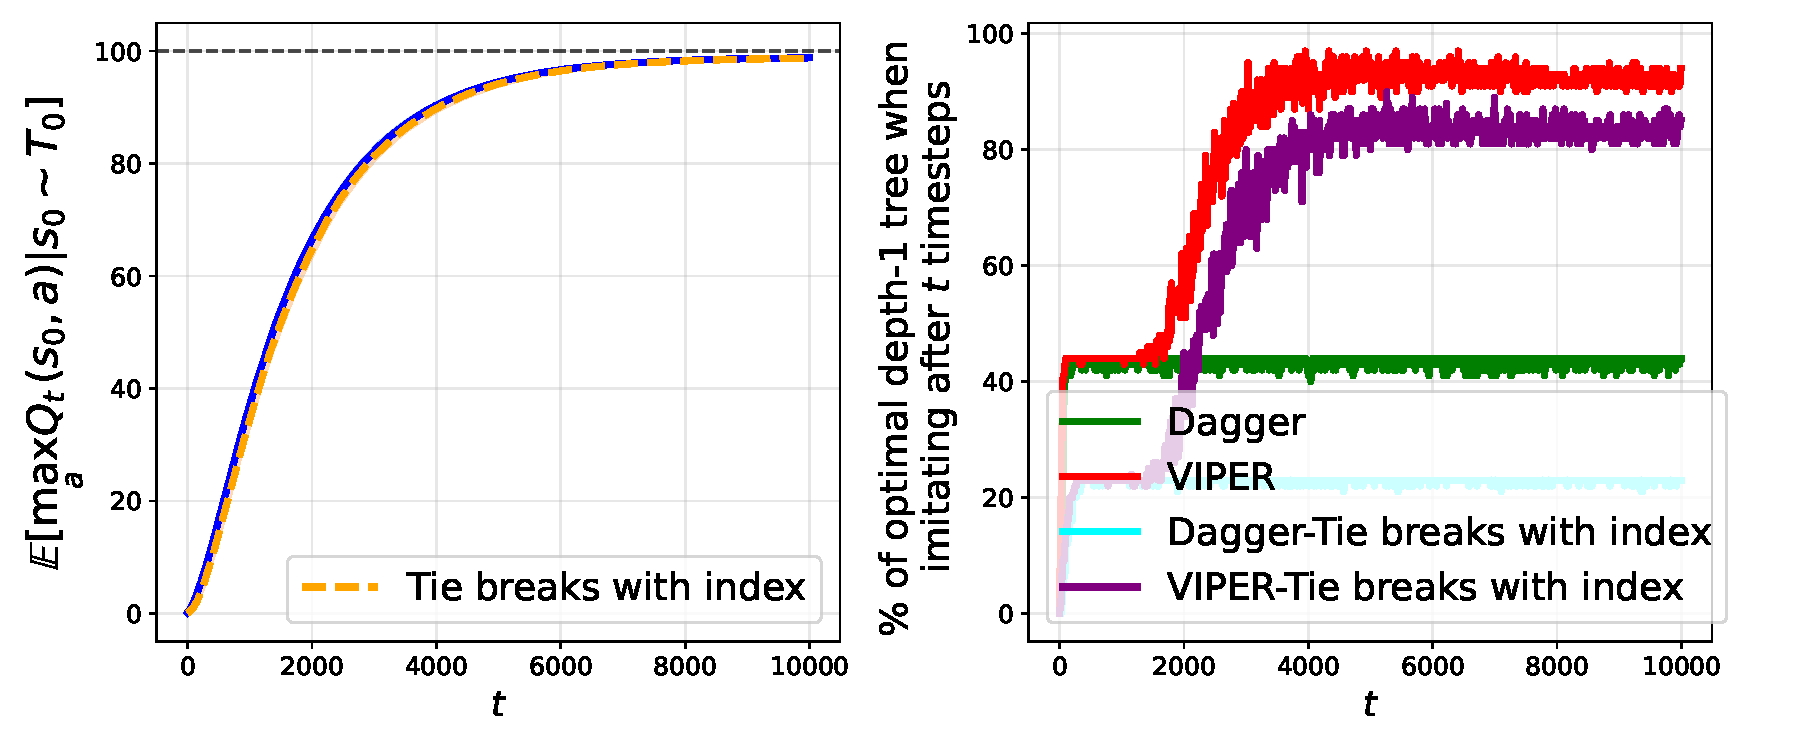
\includegraphics[width=1\textwidth]{images/images_part1/base_mdp.pdf}
    \caption{Left, sample complexity curve of Q-learning with default hyperparameters on the $2\times 2$ grid world MDP over 100 random seeds. Right, performance of indirect interpretable methods when imitating the greedy policy with a tree at different Q-learning stages.}\label{fig:ql-il}
\end{figure}

Now that the reader has seen how to get an interpretable policy for an MDP, we believe it is ready to dive into the contributions of this thesis.

\section{Outline of the thesis}
Throughout our thesis, we make the assumption that constraing models (e.g. policies or classifiers) to decision trees is engouh ensuring interpretability.
In this thesis we study different decision tree learning algorithms in different settings. 
In the first part of the manuscript, we show that direct decision tree learning methods~\ref{fig:direct-vs-indirect-methods} struggle to find decision tree policies even for very simple sequential decision making problems.
For that, we first reproduce the work from\cite{topin2021iterative} that presents a formalism for learning decision tree policies that optimize~\ref{def:mdp-obj} directly using reinforcement learning, and then make connexions with hardness results from the partially observable MDPs (POMDPs)\cite{POMDP,chap2} litterature.
We defer the introduction of POMDPs to later sections.
In the second part of the manuscript, we formulate decision tree induction for supervised learning as solving a sequential decision making problem.
By formalizing decision tree induction for objective\ref{def:sl} as solving an MDP~\ref{def:mdp}, we design novel algorithms that achieve very good performances.

In the last part of the text, we lift our assumption about decision tree learning guaranteeing interpretability and study other model classes.
In particular, we leverage the simplicity of \textit{indirect} methods~\ref{fig:direct-vs-indirect-methods} to imitate neural network experts with models from~\ref{fig:interpretability-performance-tradeoff} and and perform a large-scale empirical study of the interpretability-performances trade-offs on various sequential decision making tasks.
% In Table~\ref{tab:summary-parts} we summarize the outline of this manuscript in terms of learning objective (~\ref{def:sl},~\ref{def:mdp-obj}, or~\ref{def:il}) and model class (figure~\ref{fig:interpretability-performance-tradeoff}).

% \begin{table}
%     \centering
%     \begin{tabular}{|l|c|c|c|c|}
%         \hline
%          & \textbf{Decision Trees} & \textbf{Linear} & \textbf{Ensembles} & \textbf{Neural Networks} \\
%         \hline
%         Supervised Learning & Part II &  & Part II & Part II\\
%         \hline
%         Reinforcement Learning & Part I, III & Part III & & Part I, III \\
%         \hline
%         Imitation Learning & Part I, III & Part III & & Part III \\
%         \hline
%     \end{tabular}
%     \caption{Summary of objectives and model classes studied in this manuscript.}
%     \label{tab:summary-parts}
% \end{table}

We summarize our results as follows:

\begin{enumerate}
    \item Direct reinforcement learning of decision tree policies is hard because it involves POMDPs.
    \item One can use dynamic programming in MDPs to induce highly performing decision tree classifiers and regressors.
    \item In practice, controlling MDPs with interpretable policies does not necessarily decrease performances.
\end{enumerate}

% \begin{figure}
%     \centering
%     \begin{tikzpicture}[
%         bubble/.style={rectangle, rounded corners=15pt, draw, thick, fill=blue!20, text width=3.5cm, text centered, minimum height=1.5cm, font=\small},
%         arrow/.style={->, thick},
%         label/.style={font=\footnotesize, text width=3cm, text centered}
%     ]
        
%         % Define the three vertices of the triangle
%         % Top bubble - chapter 1
%         \node[bubble] (ch1) at (0,4) {Part 1\\Direct learning of interpretable policies for MDPs};
        
%         % Bottom left bubble - chapter 2  
%         \node[bubble] (ch2) at (-4,0) {Part 2\\Supervised learning of decision tree classifiers with MDPs};
        
%         % Bottom right bubble - chapter 3
%         \node[bubble] (ch3) at (4,0) {Part 3\\Indirect learning of interpretable policies to compare different model classes};
        
%         % Arrow from chapter 1 to chapter 2
%         \draw[arrow] (ch1.south west) -- (ch2.north);
%         \node[label] at (-4.5,2.5) {Too difficult, let us assume uniform transitions};
        
%         % Arrow from chapter 1 to chapter 3  
%         \draw[arrow] (ch1.south east) -- (ch3.north);
%         \node[label] at (4.5,2.5) {Too difficult, let us use indirect approach};

%         % Arrow from chapter 1 to chapter 3  
%         \draw[arrow] (ch2.east) -- (ch3.west);
%         \node[label] at (0,1.1) {Use new decision tree induction to learn better interpretable policies};
        
        
%     \end{tikzpicture}
%     \caption{Thesis structure showing the progression from direct reinforcement learning of decision tree policies (chapter 1) to simplified approaches: supervised learning with uniform transitions (chapter 2) and indirect learning methods (chapter 3).}
%     \label{fig:thesis-outline}
% \end{figure}
%
% Chapitres ordinaires (avec parties éventuelles)
%%%%%%%%%%%%%%%%%%%%%%%%%%%%%%%%%%%%%%%%%%%%%%%%%%%%%%%%%%%%%%%%%%%%%%%%%%%%%%%
%
% Première partie éventuelle
\part{A difficult problem: Learning Decision Trees for MDP}
% 
% Premier chapitre
\chapter{Introduction}\label{sec:intro-pomdp}
In the first part of the manuscript, we show that direct reinforcement learning of decision tree policies for MDPs, i.e. learning a decision tree that optimizes (\ref{def:mdp-obj}) is often very difficult.
In particular, we provide some insights as to why it is so difficult and show that indirect imitation of a neural network policy (Sec. \ref{sec:imit}), while not optimizing (\ref{def:mdp-obj}) directly, often yields very good tree policies in practice.

This first part of the manuscript is organised as follows.
In this Chapter we present, Topin et. al. \cite{topin2021iterative} framework for direct reinforcement learning of decision tree policies.
In Chapter \ref{sec:topin}, we reproduce experiments from Topin et. al. where we compare direct deep reinforcement learning (Sec. \ref{sec:drl}) of decision tree policies to indirect imitation of a neural network policy with a decision tree for the simple CartPole MDP.
In Chapter \ref{sec:pomdp}, we show that the direct approach proposed by Topin et. al. is equivalent to learning a deterministic memoryless policy for partially observable MDP (POMDP)\cite{POMDP,chap2} and show that this might be the biggest source of hardness.
In Chapter \ref{sec:pomdp-classif}, we further support this claim by constructing special instances of Topin et. al. in which the POMDPs are virtually fully observable, and show that in those cases, direct reinforcement learning of decision tree works well.  

\section{Learning Decision Tree policies for MDPs}
In the introductory example~\ref{sec:limits-il}, we have shown that imitation learning that optimizes the objective (\ref{def:il}) rather than the RL objective~\ref{def:mdp-obj}, are, unsuprisingly, prone tosub-optimality w.r.t. the lattter objective.
This motivates the study and development of \textit{direct} decision tree learning algorithms.
There already exist such algorithms that return decision tree policies optimizing the RL objective for a given MDP.
Those algorithms either learn parametric trees or non-parametric trees.

Parametric trees are not ``grown'' from the root by iteratively adding internal or leaf nodes (cf. Fig. \ref{fig:dt}), but are rather ``optimized'': the depth, internal nodes arrengement, and state-features to consider in each nodes are fixed \textit{a priori} and only the thresholds of each nodes are learned similar to doing gradient descent on neural network weights.
As the reader might have guessed, those parametric trees are advantageous in that they can be learned with the policy gradient \cite{pg_sutton}. Both \cite{silva}, \cite{vos2024optimizinginterpretabledecisiontree} and \cite{sympol} use PPO \cite{ppo} to optimize such differentiable decision trees. In particular, \cite{sympol} explicitely studies the gap in performances between their direct optimization and the indirect imitation.
While those methods optimize the RL objective (\ref{def:mdp-obj}) directly and train high-performing policies w.r.t. the downstream tasks, in general a user cannot know \textit{a priori}  what a ``good'' tree policy structure should be for a particular MDP: either the specified structure is too deep and pruning will be required after training or the tree structure is not expressive enough to encode a good policy, i.e. parametric trees cannot trade off interpretability and performances during training.
Furthermore, authors from \cite{sympol} show that extra stabilizing tricks, such as adaptive batch sizes, are required during training to outperform indirect imitation in terms of RL objective (\ref{def:mdp-obj}).

Non-parametric trees are the standard model in supervised learning \cite{breiman1984classification,ID3,c45} and offer good trade-off between interpretability and performances when optimizing (\ref{def:sl}).
On the other hand, to the best of our knowledge, there exists onlye one work studying non-parametric trees to optimize a trade-off between interpretability and the RL objective (\ref{def:mdp-obj}): Topin et. al. \cite{topin2021iterative}.

Given an MDP for which one wants to learn a decision tree policy, Topin et. al. introduced iterative bouding Markov decision processes (IBMDPs) that are an augmented version of this base MDP with more state features, more actions, additional rewards that trade-off between the RL objective and number of added nodes, and additional transitions.
Authors showed that using RL to learn certain policies in IBMDPs is equivalent to growing a tree that optimizes a trade-off between interpretability and the RL objective (\ref{def:mdp-obj}) w.r.t. the MDP of interest.

There also exists more specialized approaches that can return decision tree policies only for small problem classes.
In \cite{dt-maze}, authors prove that for maze-like MDPs, there always exist an optimal decision tree policy w.r.t. \ref{def:mdp-obj} and provide an algorithm to find it. 
Finally, in \cite{dt-opt-mdp}, authors study decision tree policies for planning in MDPs, i.e., when the transitions and rewards are known.
In the next section we present IBMDPs as introduced in Topin et. al.\cite{topin2021iterative}.

\section{Iterative Bounding Markov Decision Processes}\label{sec:ibmdp}

The key thing to know about IBMDPs is that they are, as their name suggests, MDPs.
Hence, IBMDPs admits an optimal deterministic Markovian policy for problem (\ref{def:mdp-obj}).
In this part we will assume that all the MDP we consider are factored MDPs \ref{def:fmdp} with a finite set of actions, so we use bold fonts for states and observations as they are vector-valued.
However all our results generalize to discrete states (in $\mathbb{Z}^m$) MDP that we can factor using one-hot encodings. 
Given an MDP for which we want to learn a decision tree policy, that we call the base MDP, the states in an associated IBMDP are concatenations of the base MDP states and some observations. 
Those observations are information about the base states that are refined--``iteratively bounded''-- at each step and represent a subspace of the base MDP state space.
Actions available in an IBMDP are the actions of the base MDP, that change the state of the latter, and \textit{information gathering} actions that change the observation part of the IBMDP state.
Now, taking base actions in an IBMDP is rewarded like in the base MDP, this ensures that the base objective, e.g. balancing the pole or treating cancer, is still encoded in the IBMDP reward.
When taking an information gathering action, the reward is an arbitrary value such that optimizing (\ref{def:mdp-obj}) in the IBMDP is equivalent to optimizing some trade-off between \ref{def:mdp-obj} in the base MDP and interpretability.
 
Before showing how to get decision tree policies from IBMDP policies, we give a formal definition of IBMDPs following Topin et. al.~\cite{topin2021iterative}.

\begin{definition}[Iterative Bounding Markov decision process]\label{def:ibmdp}
Given a \textit{factored} MDP $\mathcal{M}$ $\langle S, A, R, T, T_0 \rangle$ (\ref{def:fmdp}), an associated iterative bouding Markov decision process $\mathcal{M}_{IB}$ is a tuple:
\begin{align*}
    \langle \overbrace{S \times O}^{\text{State space}}, \underbrace{A \cup A_{info}}_{\text{Action space}}, \overbrace{(R, \zeta)}^{\text{Reward function}}, \underbrace{(T_{info}, T, T_0)}_{\text{Transitions}}\rangle
\end{align*}

\begin{itemize}
\item $S$ is the base MDP factored state space. A state $\boldsymbol{s} = (s_1, \dots, s_n)\in S$ has $n$ bounded features $s_i \in [L_i, U_i]$ where $\infty < L_i \leq U_i < \infty \forall 1\leq i \leq n$.
\item $O$ are the observations in an IBMDP. They are partial information about the base MDP state features. The set of observations is the current features bounds: $O\subsetneq S^2 =  [L_1, U_1]\times \dots \times [L_n, U_n] \times [L_1, U_1]\times \dots \times [L_n, U_n]$. So the complete IBMDP state space is $S \times O$, the concatenations of base state features and observations.
\item $A$ is the base MDP actions set.
\item $A_{info}$ are \textit{information gathering} actions (IGAs) of the form $\langle i, v \rangle$ where $i$ is a state feature index $1 \leq i \leq n$ and $v$ is a real number. So the complete action space of an IBMDP is the set of base MDP actions and information gathering actions $A \cup A_{info}$.
\item $R: S\times A \rightarrow \mathbb{R}$ is the base MDP reward function.
\item $\zeta$ is a reward signal for taking an information gathering action.
So the IBMDP reward function is to get a reward from the base MDP if the action is a base MDP action or to get $\zeta$ if the action is an IGA action.
\item $T_{info}: S\times O \times( A_{info} \cup A )\rightarrow \Delta (S\times O)$ is the transition kernel of IBMDPs: 
Given some observation $\boldsymbol{o}_t = (L'_1, U'_1, \dots, L'_n, U'_n) \in O$ and state features $\boldsymbol{s}_t=(s'_1, s'_2, \dots, s'_n)$ if an IGA $\langle i, v \rangle$ is taken, the new observation is:
\begin{align*}
    \boldsymbol{o}_{t+1} &= \begin{cases}
        (L'_1, U'_1, \dots , L'_i, \min\{v, U'_i\}, \dots , L''_n, U'_n) \text{ if } s_i \leq v\\
        (L'_1, U'_1, \dots , \max\{v, L'_i\}, U'_i, \dots , L''_n, U'_n) \text{ if } s_i > v
    \end{cases}
\end{align*}
If a base action $a_t\in A$ is taken, the new observation is reset to the default state bounds $(L_1, U_1,\dots, L_n, U_n)$ and the state features change according to the base MDP transitition kernel: $\boldsymbol{s}_{t+1}\sim T(\boldsymbol{s}_t, a_t)$.
At initialization, the base state features are drawn from the base MDP $T_0$ and the observation is always set to the default state features bounds $\boldsymbol{o}_0=(L_1, U_1,\dots, L_n, U_n)$.
\end{itemize}
\end{definition}

Now remains to extract a decision tree policy for MDP $\mathcal{M}$ from a policy for an associated IBMDP $\mathcal{M}_{IB}$. 

\subsection{From Policies to Trees}

One can notice that information gathering actions (\ref{def:ibmdp}) resemble the Boolean functions that make up internal decision tree nodes (cf. Figure \ref{fig:dt}).
Indeed, a policy taking actions in an IBMDP essentially builds a tree by taking sequences of IGAs (internal nodes) and then a base action in the base MDP (leaf node) and repeats this process over time.
In particular, the IGA rewards $\zeta$ can be seen as a regularization or a penalty for interpretabiliy: if $\zeta$ is very low compared to base rewards, a policy will try to act in the base MDP as often as possible, i.e. build shallow trees that short paths between root and leaves.

Authors from \cite{topin2021iterative} show that not all IBMDP policies are decision tree policies.
In particular, they show that only deterministic policies depending solely on the observation part of the IBMDP states are guaranteed to correspond to decision tree policies for the base MDP.
The intuition is that if one trains a policy $\pi:S\timesO\rightarrow A\cup A_{info}$, the policy might learn to rely only on state features of the base MDP $\boldsymbol{s}$ and take only base actions (no IGAs) which would simply be any policy for the base MDP.

\begin{proposition}[Deterministic partially observable IBMDP policies are decision trees]\label{def:po-policy}
    Given a factored MDP $\mathcal{M}$ $\langle S, A, R, T, T_0\rangle$ (\ref{def:fmdp}) and an associated IBMDP $\mathcal{M}_{IB}$ $\langle S \times O,A \cup A_{info}, (R, \zeta), (T_{info}, T, T_0)\rangle$ (\ref{def:ibmdp}), a deterministic partially observable policy $\pi_{po}: O \rightarrow A\cup A_{info}$ is a decision tree policy $\pi_{\mathcal{T}}: S \rightarrow A$ for the base MDP $\mathcal{M}$.
\end{proposition}

\begin{proof}(Sketch) Algorithm~\ref{alg:extract-tree} that takes as input a deterministic partially observable policy (\ref{def:po-policy}) for an IBMDP $\mathcal{M}_{IB}$ $\langle S \times O,A \cup A_{info}, (R, \zeta), (T_{info}, T, T_0)\rangle$ (\ref{def:ibmdp}), returns a decision tree policy $\pi_{\mathcal{T}}$ (\ref{def:dt}) for $\mathcal{M}$ $\langle S, A, R, T, T_0\rangle$ and always terminates unless the deterministic partially observable policy only takes IGAs.
\end{proof}

\begin{algorithm}[t]
    \KwData{Deterministic partially observable policy $\pi_{po}$ for IBMDP $ \langle S \times O,A \cup A_{info}, (R, \zeta), (T_{info}, T, T_0)\rangle$ and observation IBMDP $\boldsymbol{o}=(L'_1, U'_1, \dots, L'_n, U'_n)$}
    \KwResult{Decision tree policy $\pi_{\mathcal{T}}$ for MDP $\langle S, A, R, T, T_0\rangle$}
    
    \SetKwProg{Fn}{Function}{:}{}
    \SetKwFunction{SubtreeFromPolicy}{Subtree\_From\_Policy}
    
    \Fn{\SubtreeFromPolicy{$\boldsymbol{o}, \pi_{po}$}}{
        $a \leftarrow \pi_{po}(\boldsymbol{o})$ \\
        \If{$a \in A_{info}$}{
            \Return Leaf\_Node(action: $a$) \Comment{// Leaf if base action}
        }
        \Else{
            $\langle i, v\rangle \leftarrow a$ \Comment{// Splitting action is feature and value} \\
            $\boldsymbol{o}_L \leftarrow \boldsymbol{o}; \quad \boldsymbol{o}_R \leftarrow \boldsymbol{o}$ \\
                         $\boldsymbol{o}_L \leftarrow (L'_1, U'_1, \dots, L'_i, v, \dots, L'_n, U'_n); \quad \boldsymbol{o}_R \leftarrow (L'_1, U'_1, \dots, v, U'_i, \dots, L'_n, U'_n)$ \\
            $child_L \leftarrow$ Subtree\_From\_Policy$(\boldsymbol{o}_L, \pi_{po})$ \\
            $child_R \leftarrow$ Subtree\_From\_Policy$(\boldsymbol{o}_R, \pi_{po})$ \\
            \Return Internal\_Node(feature: $i$, value: $v$, children: $(child_L, child_R)$)
        }
    }
    \caption{Extract a Decision Tree Policy}\label{alg:extract-tree}
\end{algorithm}

While the connexions with partially observable MDPs~\cite{POMDP,chap2} is obvious, we defer the implications to Chapter \ref{sec:pomdp} as this connexion was not make in the original IBMDP paper~\cite{topin2021iterative}.
Next we present an example of an IBMDP policy that is a decision tree for the base MDP.

\subsection{Example: an IBMDP for a grid world}
For the sake of example, we re-formulate the example MDP (\ref{example:grid}) as a factored MDP with a finite number of vector valued states ($x,y$-coordinates).
The states are $S = \{(0.5, 0.5), (0.5, 1.5), (1.5, 1.5), (1.5, 0.5)\}\subsetneq [0, 2] \times [0, 2]$.
The actions are the cardinal directions $A = \{\rightarrow, \leftarrow, \downarrow, \uparrow\}$ that shift the states by one as long as the coordinates remain in the grid.
The reward for taking any action is 0 except when in the bottom right state $(1.5, 0.5)$ which is an absorbing state: once in this state, you stay there forever. 
Optimal deterministic tabular policies were presented for this MDP in Example (\ref{example:grid}).

Suppose an associated IBMDP (\ref{def:ibmdp}) with two IGAs:
\begin{itemize}
    \item $\langle x, 1\rangle$ that tests if $x\leq 1$
    \item $\langle y, 1\rangle$ that tests if $y\leq 1$
\end{itemize}
The initial observation is always the grid bounds $\boldsymbol{o}_0=(0, 2, 0, 2)$ because a state in the grid world is always in $[0, 2] \times [0, 2]$.
There are only finitely many observations since with those two IGAs there are only nine possible observations that can be attained from $\boldsymbol{o}_0$ following the IBMDP transitions (\ref{def:ibmdp}).
For example when the IBMDP initial state features are $\boldsymbol{s}_0 = (0.5, 1.5)$, and taking first $\langle x, 1\rangle$ then $\langle y, 1\rangle$ the corresponding observations are first $\boldsymbol{o}_{t+1} = (0, 1, 0, 2)$ and then $\boldsymbol{o}_{t+2} = (0, 1, 1, 2)$.
The full observation set is $O = \{(0, 2, 0, 2), (0, 1, 0, 2), (0, 2, 0, 1), (0, 1, 0, 1), (1, 2, 0, 2), (1, 2, 0, 1), (1, 2, 1, 2), (0, 1, 1, 2), (0, 2, 1, 2)\}$.
The transitions and rewards are given by definition (\ref{def:ibmdp}).

In Figure (\ref{example:ibmdp}) we show a trajectory in this IBMDP.
\begin{figure}[h]
\centering
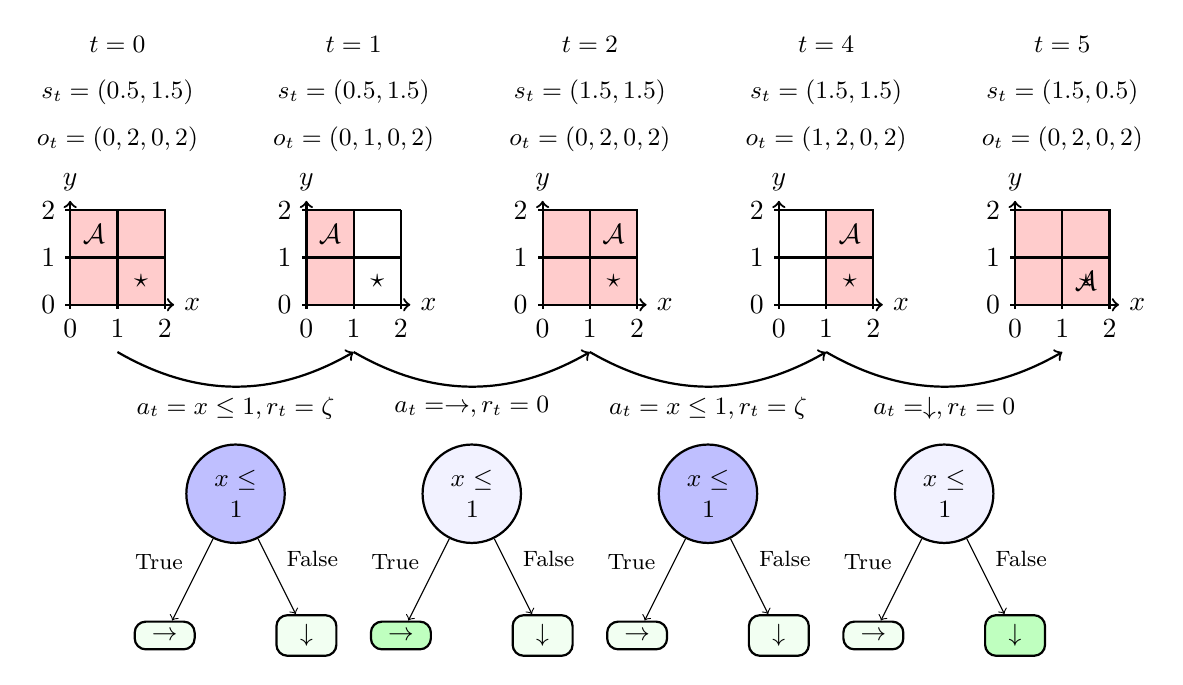
\begin{tikzpicture}[scale=0.6]
    % Define styles
    \tikzstyle{grid}=[draw, thick, fill=gray!10]
    \tikzstyle{rectangle}=[draw, thick, fill=red!20]
    
    % Row 1: IBMDP States (s, o)
    % t=0: Initial state
    \node at (2,9.5) {\small $t=0$};
    \node at (2,8.5) {\small $\boldsymbol{s}_t=(0.5, 1.5)$};
    \node at (2,7.5) {\small $\boldsymbol{o}_t=(0, 2, 0, 2)$};

    \draw[rectangle] (1,4) rectangle (3,6);
    \draw[grid] (1,4) grid (3,6);
    % Add axes
    \draw[thick, ->] (1,4) -- (3.2,4) node[right] {$x$};
    \draw[thick, ->] (1,4) -- (1,6.2) node[above] {$y$};
    \foreach \x in {0,1,2} {
        \draw[thick] (\x+1,4) -- (\x+1,3.9) node[below] {$\x$};
    }
    \foreach \y in {0,1,2} {
        \draw[thick] (1,\y+4) -- (0.9,\y+4) node[left] {$\y$};
    }
    \node at (1.5, 5.5) {$\mathcal{A}$};
    \node at (2.5, 4.5) {$\star$};
    
    % Curved arrow from t=0 to t=1
    \draw[thick, ->] (2,3) to[bend right=30] node[midway, below] {\small $a_t = x \leq 1, r_t = \zeta$} (7,3);

    % % t=1: After AIG x≤0.5
    \node at (7,9.5) {\small $t=1$};
    \node at (7,8.5) {\small $\boldsymbol{s}_t=(0.5, 1.5)$};
    \node at (7,7.5) {\small $\boldsymbol{o}_t=(0, 1, 0, 2)$};

    \draw[rectangle] (6,4) rectangle (7,6);
    \draw[grid] (6,4) grid (8,6);
    % Add axes
    \draw[thick, ->] (6,4) -- (8.2,4) node[right] {$x$};
    \draw[thick, ->] (6,4) -- (6,6.2) node[above] {$y$};
    \foreach \x in {0,1,2} {
        \draw[thick] (\x+6,4) -- (\x+6,3.9) node[below] {$\x$};
    }
    \foreach \y in {0,1,2} {
        \draw[thick] (6,\y+4) -- (5.9,\y+4) node[left] {$\y$};
    }
    \node at (6.5, 5.5) {$\mathcal{A}$};
    \node at (7.5, 4.5) {$\star$};


    % Curved arrow from t=1 to t=2
    \draw[thick, ->] (7,3) to[bend right=30] node[midway, below] {\small $a_t = \rightarrow, r_t  = 0$}(12,3);

    \node[circle, draw, thick, fill=blue!25, text width=2em, text centered, minimum height=1.5em, font=\small] (tree4_root) at (4.5,0) {$x \leq 1$};
    \node[rectangle, draw, thick, fill=green!5, text width=1.5em, text centered, rounded corners, minimum height=1em, font=\small] (tree4_right) at (3,-3) {$\rightarrow$};
    \node[rectangle, draw, thick, fill=green!5, text width=1.5em, text centered, rounded corners, minimum height=1em, font=\small] (tree4_left) at (6,-3) {$\downarrow$};
    \draw[->] (tree4_root) -- (tree4_right) node[font=\footnotesize, midway, above left] {True};
    \draw[->] (tree4_root) -- (tree4_left) node[font=\footnotesize, midway, above right] {False};

    \node at (12,9.5) {\small $t=2$};
    \node at (12,8.5) {\small $\boldsymbol{s}_t=(1.5, 1.5)$};
    \node at (12,7.5) {\small $\boldsymbol{o}_t=(0, 2, 0, 2)$};
    
    \draw[rectangle] (11,4) rectangle (13,6);
    \draw[grid] (11,4) grid (13,6);
    % Add axes
    \draw[thick, ->] (11,4) -- (13.2,4) node[right] {$x$};
    \draw[thick, ->] (11,4) -- (11,6.2) node[above] {$y$};
    \foreach \x in {0,1,2} {
        \draw[thick] (\x+11,4) -- (\x+11,3.9) node[below] {$\x$};
    }
    \foreach \y in {0,1,2} {
        \draw[thick] (11,\y+4) -- (10.9,\y+4) node[left] {$\y$};
    }
    \node at (12.5, 5.5) {$\mathcal{A}$};
    \node at (12.5, 4.5) {$\star$};
    
    % Curved arrow from t=2 to t=4
    \draw[thick, ->] (12,3) to[bend right=30] node[midway, below] {\small $a_t = x \leq 1, r_t = \zeta$} (17,3);

    \node[circle, draw, thick, fill=blue!5, text width=2em, text centered, minimum height=1.5em, font=\small] (tree4_root) at (9.5,0) {$x \leq 1$};
    \node[rectangle, draw, thick, fill=green!25, text width=1.5em, text centered, rounded corners, minimum height=1em, font=\small] (tree4_right) at (8,-3) {$\rightarrow$};
    \node[rectangle, draw, thick, fill=green!5, text width=1.5em, text centered, rounded corners, minimum height=1em, font=\small] (tree4_left) at (11,-3) {$\downarrow$};
    \draw[->] (tree4_root) -- (tree4_right) node[font=\footnotesize, midway, above left] {True};
    \draw[->] (tree4_root) -- (tree4_left) node[font=\footnotesize, midway, above right] {False};

    
    \node at (17,9.5) {\small $t=4$};
    \node at (17,8.5) {\small $\boldsymbol{s}_t=(1.5, 1.5)$};
    \node at (17,7.5) {\small $\boldsymbol{o}_t=(1, 2, 0, 2)$};

    \draw[rectangle] (17,4) rectangle (18,6);
    \draw[grid] (16,4) grid (18,6);
    % Add axes
    \draw[thick, ->] (16,4) -- (18.2,4) node[right] {$x$};
    \draw[thick, ->] (16,4) -- (16,6.2) node[above] {$y$};
    \foreach \x in {0,1,2} {
        \draw[thick] (\x+16,4) -- (\x+16,3.9) node[below] {$\x$};
    }
    \foreach \y in {0,1,2} {
        \draw[thick] (16,\y+4) -- (15.9,\y+4) node[left] {$\y$};
    }
    \node at (17.5, 5.5) {$\mathcal{A}$};
    \node at (17.5, 4.5) {$\star$};
    
    \draw[thick, ->] (17,3) to[bend right=30] node[midway, below] {\small $a_t = \downarrow, r_t = 0$} (22,3);
    
    \node[circle, draw, thick, fill=blue!25, text width=2em, text centered, minimum height=1.5em, font=\small] (tree4_root) at (14.5,0) {$x \leq 1$};
    \node[rectangle, draw, thick, fill=green!5, text width=1.5em, text centered, rounded corners, minimum height=1em, font=\small] (tree4_right) at (13,-3) {$\rightarrow$};
    \node[rectangle, draw, thick, fill=green!5, text width=1.5em, text centered, rounded corners, minimum height=1em, font=\small] (tree4_left) at (16,-3) {$\downarrow$};
    \draw[->] (tree4_root) -- (tree4_right) node[font=\footnotesize, midway, above left] {True};
    \draw[->] (tree4_root) -- (tree4_left) node[font=\footnotesize, midway, above right] {False};


    \node at (22,9.5) {\small $t=5$};
    \node at (22,8.5) {\small $\boldsymbol{s}_t=(1.5, 0.5)$};
    \node at (22,7.5) {\small $\boldsymbol{o}_t=(0, 2, 0, 2)$};
 
    \draw[rectangle] (21,4) rectangle (23,6);
    \draw[grid] (21,4) grid (23,6);
    % Add axes
    \draw[thick, ->] (21,4) -- (23.2,4) node[right] {$x$};
    \draw[thick, ->] (21,4) -- (21,6.2) node[above] {$y$};
    \foreach \x in {0,1,2} {
        \draw[thick] (\x+21,4) -- (\x+21,3.9) node[below] {$\x$};
    }
    \foreach \y in {0,1,2} {
        \draw[thick] (21,\y+4) -- (20.9,\y+4) node[left] {$\y$};
    }
    \node at (22.5, 4.5) {$\mathcal{A}$};
    \node at (22.5, 4.5) {$\star$};

    \node[circle, draw, thick, fill=blue!5, text width=2em, text centered, minimum height=1.5em, font=\small] (tree4_root) at (19.5,0) {$x \leq 1$};
    \node[rectangle, draw, thick, fill=green!5, text width=1.5em, text centered, rounded corners, minimum height=1em, font=\small] (tree4_right) at (18,-3) {$\rightarrow$};
    \node[rectangle, draw, thick, fill=green!25, text width=1.5em, text centered, rounded corners, minimum height=1em, font=\small] (tree4_left) at (21,-3) {$\downarrow$};
    \draw[->] (tree4_root) -- (tree4_right) node[font=\footnotesize, midway, above left] {True};
    \draw[->] (tree4_root) -- (tree4_left) node[font=\footnotesize, midway, above right] {False};

    
\end{tikzpicture}
\caption{An IBMDP trajectory when the base MDP is 2$\times$2 grid world, and equivalent decision tree policy traversal.
$\mathcal{A}$ indicates the current state $\boldsymbol{s}_t$ in the grid.
The pink obstructions of the grid represent the current partial observations $\boldsymbol{o}_t$ of the state features.
When the pink covers the whole grid, the information contained in the observation is ``the current state could be anywhere in the grid''.
The more Information gathering actions are taken, the more refined the bounds on the current state features get.
At $t=0$, the state features are $\boldsymbol{s}_0 = (0.5, 1.5)$. 
The initial observation is always the base MDP default feature bounds, here $\boldsymbol{o}_0=(0, 2, 0, 2)$ because the base states are in $[0, 2] \times [0, 2]$.
The first action is an IGA that tests the feature $x$ of the states against the value $1$ and the reward $\zeta$. 
This transition corresponds to going through an internal node in a decision tree policy as illustrated in the figure. 
At $t=1$, after gathering the information that the $x$-value of the current base state is below 1, the observation is updated with the refined state bounds $\boldsymbol{o}_1=(0, 1, 0, 2)$, i.e. the pink area shrinks, and the base state features remain unchanged.
The agent then takes a base action that is to move right. 
This gives a reward 0, resets the observation to the original bounds, and changes the base state to $\boldsymbol{s}_2=(1.5, 1.5)$. And the trajectory continues like this until the agent reaches the absorbing base state $\boldsymbol{s}_5=(1.5, 0.5)$.}
\label{example:ibmdp}
\end{figure}

\section{Summary}
In this chapter, we presented the approach of Topin et. al.~\cite{topin2021iterative} to find decision tree policies that directly trade off interpretability and the RL objective (\ref{def:mdp-obj}) rather than the surrogate imitation loss (\ref{def:il}).
To achieve that Topin et. al. showed that deterministic partially observable policy in some MDP, an IBMDP (\ref{def:ibmdp}).

The promise of Topin et. al. is that optimizing (\ref{def:mdp-obj}) in an IBMDP trades off naturally the base MDP rewards and the interpretability of the policy through the reward signal $\zeta$.

We can thus write an interpretable RL objective as follows:
\begin{definition}[direct interpretable RL objective]\label{def:irl}
    Given a factored MDP $\mathcal{M} \langle S, A, R, T, T_0 \rangle$ for which we want an interpretable policy, e.g. a decision tree, a discount factor $\gamma \in (0,1]$, some interpretability penalty $\zeta$, and a set of information gathering actions $A_{info}$, we solve:
\begin{align*}
    \pi^\star_{po} &= \underset{\pi_{po}}{\opertarname{argmax}} \mathbb{E}\left[\sum_{t=0}^{\infty} \gamma^t R((\boldsymbol{s}_t, \boldsymbol{o}_t), a_t) \mid \boldsymbol{s}_0 \sim T_0, a_t = \pi_{po}(\boldsymbol{o}_t), \boldsymbol{s}_{t+1} \sim T(\boldsymbol{s}_t, a_t), \boldsymbol{o}_{t+1}\sim T(\boldsymbol{o_t}, a_t)\right]\\
    &= \underset{\pi_{po}}{\operatorname{argmax}} \mathbb{E}[V^{\pi_{po}}(s_0, o_0)| s_0\sim T_0]
\end{align*}
With $V^{\pi_{po}}$ the value function (\ref{def:vs}) of deterministic partially observable policy $\pi_{po}: O \rightarrow A\cup A_{info}$ (\ref{def:po-policy}) in the IBMDP $\mathcal{M}_{IB}$ $\langle S \times O,A \cup A_{info}, (R, \zeta), (T_{info}, T, T_0)\rangle$ (\ref{def:ibmdp}).
\end{definition}

After optimizing objective (\ref{def:irl}) with, e.g. reinforcement learning, we thus use Algorithm \ref{alg:extract-tree} to obtain a decision tree policy that trades off between interpretability and the RL objectvie (\ref{def:mdp-obj}) for our MDP of intereset.
This is exactly what we do in the next chapters.
% In Figure (\ref{fig:summary-ibmdp}) we summarize the direct reinforcement learning approach of Topin et. al. that we use in the next chapters. 
% \begin{figure}[h]
%     \centering
%     \begin{tikzpicture}
%         \draw[fill=blue!30] (0, 0) rectangle (5.9, 3);
%         \node at (3, 2.5) {IBMDP $\mathcal{M}_{IB} \langle \mathcal{M}, O, A_{info}, \zeta, T_{info}\rangle$};
%         \draw[fill=blue!10] (0, 0) rectangle (5, 2);
%         \node at (3, 1.5) {MDP $\mathcal{M} \langle S, A, R, T, T_0 \rangle$};
        
%         \draw[fill=red!10] (10, 0) rectangle (14, 3);
%         \node at (12, 2) {\textbf{Objective}};
%         \node at (12, 1) {$\pi^{\star}_{po} = \underset{\pi_{po}}{\operatorname{argmax}} \mathbb{E}[V^{\pi_{po}}(\boldsymbol{s}_0, \boldsymbal{o}_0)| \boldsymbol{s}_0\sim T_0]$};
        
%         \draw[fill=red!10] (1, -5) rectangle (5, -2);
%         \node at (3, -3) {\textbf{Decision Tree Policy}};
%         \node at (3, -4) {$\pi_{\mathcal{T}}: S \rightarrow A$};
        
%         \draw[fill=red!10] (9.5, -5) rectangle (14.5, -2);
%         \node at (12, -3) {\textbf{Deterministic Policy}};
%         \node at (12, -4) {$\pi_{po}: O \rightarrow A \cup A_{info}$};
        
%         \draw[thick, ->] (6, 2) -- (10, 2) node[midway, above] {$\gamma$};
%         \draw[thick, <-] (5, -3.5) -- (9.5, -3.5) node[midway, above] {Extract tree with Alg 6};
%         \draw[thick, ->] (12, 0) -- (12, -2) node[midway, left] {Solve with e.g. RL};
%         \draw[thick, <-] (3, 0.5) -- (3, -2) node[midway, left] {Can be interpreted};
    
        
%         % % Final arrow from tree back to base MDP - adjusted position
%         % \draw[thick, ->] (1.75, -2.5) -- (1.75, -0.5) node[midway, right] {Can deploy\\and interpret};
        
%     \end{tikzpicture}
%     \caption{A formal framework to learn decision tree policies for MDPs. This include learning a deterministic partially observable policy in a POIBMDP (cite).}
%     \label{fig:summary-ibmdp}
%     \end{figure}


%
% Deuxième chapitre
\chapter{Direct Deep Reinforcement Learning of Decision Tree Policies}\label{sec:topin}
In this chapter, we compare deep reinforcement learning of decision tree policies (Chaper \ref{sec:intro-pomdp}) to imitation learning of decision tree policies (Sec. \ref{sec:imit}) for the CartPole MDP~\cite{cartpole}.

In particular, we attempt to reproduce the results from~\cite[Table 1]{topin2021iterative} in which authors constraint the solution space of decision tree policies to depth-2 trees.
In the original results, authors find that deep reinforcement learning to solve the interpretable rl objective (\ref{def:irl}) and Dagger or VIPER (Sec. \ref{sec:imit}) to solve the imitation learning objective (\ref{def:il}) find similar decision trees.
We find that imitation learning, despite not directly optimizing the RL objective (\ref{def:mdp-obj}) for CartPole, outperforms deep RL that optimizes (\ref{def:irl}) even though the deep RL approach directly optimizes the RL objective for CartPole (up to some trade-off with interpretability).
\section{Reproducing ``Iterative Bounding MDPs: Learning Interpretable Policies via Non-Interpretable Methods''}

\subsection{IBMDP formulation}
Given a a factored base MDP $\mathcal{M}\langle S, A, R, T, T_0\rangle$ (\ref{def:fmdp}), in order to define an IBMDP $\mathcal{M}_{IB}\langle S\times O, A\cup A_{\info}, (R, \zeta),( T, T_0, T_{info})\rangle$ (\ref{def:ibmdp}), the user needs to provide the set of information gathering actions $A_{info}$ and the reward $\zeta$ for taking those.
Authors of~\cite{topin2021iterative} propose to parametrize the set of IGAs with $i \times p$ actions $\langle v_k, i \rangle$ with $v_k$ depending on the current observation $\boldsymbol{o}_t=(L'_1, U'_1, \dots, L'_i, U'_i, \dots, L'_n, U'_n)$: $v_k = \frac{k(U'_i - L'_i)}{p+1}$.
This parametric IGAs space keeps the discrete IBMDP action space at a reasonable size while providing a learning algorithm with varied IGAs to try.

For example, if we define an IBMDP with $p=3$ for the grid world from Example~\ref{example:grid}, the grid world action space is augmented with six IGAs. 
At $t=0$, recall that $\boldsymbol{o}_0=(0, 2, 0, 2)$, so if an IGA is taken, e.g. $\langle v_2, 2 \rangle$, the effective IGA is $\langle v_2=\frac{k(2-0)}{3+1}, i \rangle = \langle 1, 2 \rangle$ which in turn effectively corresponds to an internal decision tree node $y \leq 1$.
If the current state $y$-feature value is $0.5$, then the next observation at $t=1$ is $\boldsymbol{o}_1=(0, 2, 0, 1)$. At $t=2$ if $a_t=\langle v_2, 2 \rangle$ again, it would be effectively $\langle v_2=\frac{k(1-0)}{3+1}, i \rangle = \langle 0.5, 2 \rangle$. 
This would give the next observation at $t=2$ $\boldsymbol{o}_2=(0, 2, 0, 0.5)$ and so on \dots. 

Furthermore, author propose to regularize the learned decision tree policy with a maximum depth parameter $D$.
Unfortunately, authors did not describe how they implemented the depth control in their work, hence we have to try different approaches to reproduce their results.

To control the tree depth during learning in the IBMDP, we can either give negative reward for taking $D$ IGAs in a row, or we could terminate the trajectory. 
The penalization approaches can break the MDP formalism because the reward function now depends on time while it should only depend on states and actions (\ref{def:mdp}).
Similarly, the termination approach requires a transition function that depends on time which also breaks the Makrov property.

We actually find that when $p+1$, the IBMDP information gathering space parameter, is a prime number, then as a direct consequence of the \textit{Chinese Reminder Theorem}, the current tree depth is directly encoded in the current observation $\boldsymbol{o}_t$. 
Hence, when $p+1$ is prime, we can control the depth through either transitions or rewards without tracking the time.

We will try various $\zeta$, various $p$, and various depth control in our experiments but first we describe the reinforcement learning algorithms used in~\cite{topin2021iterative}.

\subsection{Modified Deep Reinforcement Learning algorithms}
Authors of \cite{topin2021iterative} use two deep reinforcement learning baselines to which they apply some modifications in order to learn partially observable policies as required by proposition (\ref{def:po-policy}) and objective (\ref{def:irl}).

The first algorithm is a modified proximal policy optimization algorithm (PPO)(\cite{ppo}, Alg. \ref{alg:ppo}) that we present in Algorithm \ref{alg:mod-ppo}.
Authors modify the standard PPO and train a neural network policy $O\rightarrow A\cup A_{info}$ while the neural network value function is $S\times O\rightarrow A\cup A_{info}$.

The second deep reinforcement learning algorithm used is the deep Q-networks algorithm (DQN)(\cite{dqn}, Alg. \ref{alg:dqn}) that we present in Algorithm \ref{alg:mod-dqn}.
A similar modification is done to DQN to return a partially observable policy. The trained $Q$-function is approximated with a neural network $O\rightarrow \rightarrow \mathbb{R}^{|A\cup A_{info}|}$ rather than $S\times O\rightarrow \mathbb{R}^{|A\cup A_{info}|}$.
In this modified DQN, the temporal difference error target for the $Q$-function $O\rightarrow A\cup A_{info}$ is approximated by a neural network $S\times O\rightarrow A\cup A_{info}$ that is in turn trained by bootstrapping the temporal difference error with itself.

Those two variants of DQN and PPO have first been introduced in \cite{pinto} for robotics tasks with partially observable components, under the name ``asymmetric'' actor-critic. 
Asymmetric RL algorithms that have policy and value estimates using different information from a POMDP~\cite{POMDP,chap2} were later studied theoretically to solve POMDPs in Baisero's work~\cite{baisero-dqn,baisero-ppo}.
The connexions from Deep RL in IBMDPs for objective \ref{def:irl} is absent from \cite{topin2021iterative} and we defer their connexions to direct interpretable reinforcement learning to the next Chapter as our primary goal is to reproduce \cite{topin2021iterative} \textit{as is}.

Next, we present the precise experimental setup we use to reproduce~\cite[Table 1]{topin2021iterative} in order to study direct deep reinforcement learning of decision tree policies for the CartPole MDP.

\begin{algorithm}
    \KwData{IBMDP $\mathcal{M}_{IB}\langle S\times O, A\cup A_{\info}, (R, \zeta),( T, T_0, T_{info})\rangle$, learning rate $\alpha$, exploration rate $\epsilon$, partially observable Q-network parameters $\theta$, Q-network parameters $\phi$, replay buffer $\mathcal{B}$, update frequency $C$}
    \KwResult{Partially pbservable deterministic policy $\pi_{po}$}
    Initialize partially observable Q-network parameters $\theta$\\
    Initialize Q-network parameters $\phi$ and target network parameters $\phi^- = \phi$ \\

    Initialize replay buffer $\mathcal{B} = \emptyset$ \\
    \For{each episode}{
        Initialize state $\boldsymbol{s}_0 \sim T_0$ \\
        Initialize state $\boldsymbol{o}_0 = (L_1, U_1, \dots, L_n, U_n)$ \\

        \For{each step $t$}{
            Choose action $a_t$ using $\epsilon$-greedy: $a_t = \arg\max_a Q_\theta(\boldsymbol{o}_t,a)$ with prob. $1-\epsilon$ \\
            Take action $a_t$, observe $r_t$ \\
            Store transition $(\boldsymbol{s}_t, \boldsymbol{o}_t, a_t, r_t, \boldsymbol{s}_{t+1})$ in $\mathcal{B}$ \\
            Sample random batch $(\boldsymbol{s}_i, \boldsymbol{o}_i, a_i, r_i, \boldsymbol{s}_{i+1}) \sim \mathcal{B}$ \\
            $a' = \underset{a}{\operatorname{argmax}} Q_{\theta}(\boldsymbol{o}_i, a)$ \\
            $y_i = r_i + \gamma Q_{\phi^-}(\boldsymbol{s}_{i+1}, a')$ \Comment{// Compute target}
            $\phi \leftarrow \phi - \alpha \nabla_\phi (Q_\phi(\boldsymbol{s}_i, a_i) - y_i)^2$ \Comment{// Update Q-network}
            $\theta \leftarrow \theta - \alpha \nabla_\theta (Q_\theta(\boldsymbol{o}_i, a_i) - y_i)^2$ \Comment{// Update partially observable Q-network}

            \If{$t \bmod C = 0$}{
                $\theta^- \leftarrow \theta$ \Comment{// Update target network}
            }
            $\boldsymbol{s}_t \leftarrow \boldsymbol{s}_{t+1}$ \\
            $\boldsymbol{o}_t \leftarrow \boldsymbol{o}_{t+1}$ \\
        }
    }
    $\pi_{po}(\boldsymbol{o}) = \arg\max_a Q_\theta(\boldsymbol{o},a)$ \Comment{// Extract greedy policy}
    \caption{Modified Deep Q-Network (DQN)}\label{alg:mod-dqn}
\end{algorithm}


\begin{algorithm}
    \KwData{IBMDP $\mathcal{M}_{IB}\langle S\times O, A\cup A_{\info}, (R, \zeta),( T, T_0, T_{info})\rangle$, learning rate $\alpha$, policy parameters $\theta$, clipping parameter $\epsilon$, value function parameters $\phi$}
    \KwResult{Partially observable stochastic policy $\pi_{po_\theta}$}
    Initialize policy parameters $\theta$ and value function parameters $\phi$ \\
    \For{each episode}{
        Generate trajectory $\tau = (\boldsymbol{s}_0, \boldsymbol{o}_0, a_0, r_0, \boldsymbol{s}_1, \boldsymbol{o}_1, a_1, r_1, \ldots)$ following $\pi_\theta$ \\
        \For{each timestep $t$ in trajectory}{
            $G_t \leftarrow \sum_{k=t}^{T} \gamma^{k-t} r_k$ \Comment{// Compute return}
            $A_t \leftarrow G_t - V_\phi(\boldsymbol{s}_t)$ \Comment{// Compute advantage}
            $r_t(\theta) \leftarrow \frac{\pi_{po_\theta}(a_t|\boldsymbol{o}_t)}{\pi_{po_\theta}_{old}(a_t|\boldsymbol{o}_t)}$ \Comment{// Compute probability ratio}
            $L^{CLIP}_t \leftarrow \min(r_t(\theta) A_t, \text{clip}(r_t(\theta), 1-\epsilon, 1+\epsilon) A_t)$ \Comment{// Clipped objective}
            $\theta \leftarrow \theta + \alpha \nabla_\theta L^{CLIP}_t$ \Comment{// Policy update}
            $\phi \leftarrow \phi + \alpha \nabla_\phi (G_t - V_\phi(\boldsymbol{s}_t))^2$ \Comment{// Value function update}
        }
        $\theta_{old} \leftarrow \theta$ \Comment{// Update old policy}
    }
    \caption{Proximal Policy Optimization (PPO)}\label{alg:mod-ppo}
\end{algorithm}

\section{Experimental setup}
\subsection{(IB)MDP} 

We use the exact same MDP and associated IBMDPs for our experiments as~\cite{topin2021iterative} except mentioned otherwise.

\paragraph{MDP} The problem is to optimize (\ref{def:mdp-obj}) with a decision tree policy for the CartPole MDP~\cite{cartpole}.
At each time step a learning algorithm observes the cart position velocity and the pole angle and angular velocity, and can take action to push the cart left or right.
While the cart is roughly balanced, i.e., while the cart angle remains in some fixed range, the agent gets a positive reward.
If the cart is out of balance; the MDP transitions to an absorbing terminal state and gets 0 reward forever.
Like in~\cite{topin2021iterative}, we use the gymnasium \texttt{CartPole-v0} implementation~\cite{gymnasium} of the CartPole MDP in which trajectories are truncated after 200 timesteps making the maximum cumulative reward, i.e. the optimal value of objective \ref{def:mdp-obj}, to be 200.
The state features of the CartPole MDP are in $[-2, 2] \times [-2, 2] \times [-0.14, 0.14] \times [-1.4, 1.4]$.

\paragraph{IBMDP} Authors define the associated IBMDP with $\zeta=-0.01$ and parametric information gathering action space defined by $p=3$.
In addition we also try $\zeta=0.01$ and $p=2$.
The discount factor used by the authors is $\gamma=1$.

We potentially differ from the original paper setting in the way we handle maximum depth limiation. 
Indeed authors restrain the learning of policies to be equivalent to depth-2 trees but don't detail how they do so.
We hence try two different approaches as mentioned in the previous secion: terminating trajectories if the agent takes too much information gathering in a row or simply giving a reward of $-1$ to the agent everytime it takes an information gathering action past the depth limit.
We will also try IBMDPs where we do not limit the maximum depth for completeness.

\subsection{Baselines}
\paragraph{Modified DQN} as mentioned above, authors use the modified version of DQN from Algorithm~\ref{alg:mod-dqn}.
We use the exact same hyperparameters for modified DQN as the authors when possible. 
We use the same layers width (128) and number of hidden layers (2), the same exploration strategy ($\epsilon$-greedy with linearly decreasing value $\epsilon$ between 0.5 and 0.05 during the first 10\% of the training),
the same replay buffer size ($10^6$) and the same number of transitions to be collected randomly before doing value updates ($10^5$).
We also try to use more exploration during training (change the initial $\epsilon$ value to 0.9).
We use the same optimizer (RMSprop with hyperparameter 0.95 and learning rate $2.5 \times 10^{-4}$) to update the $Q$-networks.

Authors did not share what DQN implementation they used so we use the stable-baselines3 one~\cite{stable-baselines3}.
Authors did not share what activations they used so we try both $\operatorname{tanh}()$ and $\operatorname{relu}()$. 

\paragraph{Modified PPO} for the modified PPO algorithm (Alg.~\ref{alg:mod-ppo}), we can exactly match the authors hyperparameters since they use the open source stable-baselines3 implementation of PPO.

We match training budgets: we train modified DQN on 1 million timesteps and modified PPO on 4 million timesteps.

\paragraph{DQN and PPO} We also benchmark the standard DQN and PPO when learning IBMDP policies $\pi:S\times O\rightarrow A\cup A_{info}$ and when learning standard $\pi:S\rightarrow A$ policies directly in the CartPole MDP.

We summarize hyperparameters for the IBMDP and for the learning algorithms in Tables \ref{tab:ibmdp-params}, \ref{tab:ibmdp-rl1} and \ref{tab:ibmdp-rl2}.

\begin{table}[h]
    \centering
    \caption{IBMDP hyperparameters. We try 12 different IBMDPs. In \textcolor{green}{green} we highlight the hyperparameters from the original paper and in \textcolor{red}{red} we highlight the hyperparameter names for which author do not give information.}\label{tab:ibmdp-params}
    \begin{tabular}{ll}
    \toprule
    \textbf{Hyperparameter} & \textbf{Values}\\
    \midrule
    Discount factor $\gamma$ & \textcolor{green}{1} \\
    Information gathering actions parameter $p$ & 2, \textcolor{green}{3} \\
    Information gathering actions rewards $\zeta$ & \textcolor{green}{-0.01}, 0.01 \\
    \textcolor{red}{Depth control} & Done signal, negative reward, none \\ 
    \bottomrule
    \end{tabular}
    \end{table}

\begin{table}[h]
    \centering
    \caption{(Modified) DQN trained on $10^6$ timesteps. This gives four different instantiation of (modified) DQN. Hyperparameters not mentioned are stable-baselines3 default. In \textcolor{green}{green} we highlight the hyperparameters from the original paper and in \textcolor{red}{red} we highlight the hyperparameter names for which author do not give information.}\label{tab:ibmdp-rl1}
    \begin{tabular}{ll}
    \toprule
    \textbf{Hyperparameter} & \textbf{Values}\\
    \midrule
    Buffer size & \textcolor{green}{$10^6$} \\
    Random transitions before learning & \textcolor{green}{$10^5$} \\
    Epsilon stard & 0.9, \textcolor{green}{0.5} \\
    Epsilon end & \textcolor{green}{0.05} \\
    Exploration fraction & \textcolor{green}{0.1} \\
    Optimizer & \textcolor{green}{RMSprop ($\alpha = 0.95$)}\\
    Learning rate & \textcolor{green}{$2.5\times10^{-4}$}\\
    Networks architectures & \textcolor{green}{[128, 128]}\\
    \textcolor{red}{Networks activation} & $\operatorname{tanh()}$, $\operatorname{relu()}$\\
    \bottomrule
    \end{tabular}
    \end{table}

\begin{table}[h]
    \centering
    \caption{(Modified) PPO trained on $4\times10^6$ timesteps. This gives two different instantiation of (modified) PPO. Hyperparameters not mentioned are stable-baselines3 default. In \textcolor{green}{green} we highlight the hyperparameters from the original paper and in \textcolor{red}{red} we highlight the hyperparameter names for which author do not give information.}\label{tab:ibmdp-rl2}
    \begin{tabular}{ll}
    \toprule
    \textbf{Hyperparameter} & \textbf{Values}\\
    \midrule
    Steps between each policy gradient steps & \textcolor{green}{512} \\
    Number of minibatch for policy gradient updates & \textcolor{green}{4} \\
    Networks architectures & \textcolor{green}{[64, 64]}\\
    \textcolor{red}{Networks activations} & $\operatorname{tanh()}$, $\operatorname{relu()}$\\
    \bottomrule
    \end{tabular}
    \end{table}


\paragraph{Indirect methods} We also compare modified RL algorithm to imitation learning (Sec. \ref{sec:imit}).
To do so, we use VIPER or Dagger (Algs~\ref{alg:viper}~\cite{dagger}, \ref{alg:viper}~\cite{viper}) to imitate greedy neural network policies obtained with standard DQN learning directly on CartPole.
And we use Dagger to imitate neural network policies obtained with the standard PPO learning directly on CartPole. 

For each indirect method, we imitate the neural network experts by fitting decision trees on 10000 expert transitions using the CART (Alg.~\ref{alg:cart}~\cite{breiman1984classification}) implementation from scikit-learn~\cite{scikit-learn} with default hyperparameters and maximum depth of 2 like in ~\cite{topin2021iterative}.
    
\subsection{Metrics}
The key metric of this section is performance when controlling the CartPole, i.e, the average \textit{undiscounted} cumulative reward of a policy on 100 trajectories (objective \ref{def:mdp-obj} with $\gamma=1$).

For modified RL algorithms that learn a partially observable policy (or $Q$-function) in an IBMPD, we periodically extract the policy (or $Q$-function) and use Alg.\ref{alg:extract-tree} to extract a decision tree for the CartPole MDP. 
We then evaluate the tree on 100 independent trajectories in the MDP and report the mean undiscounted cumulative reward.

For standard RL applied to IBMDPs, since we can't deploy learned policies directly to the base MDP as the state dimensions mismatch (such policies are $S\times O\rightarrow A \cup A_{info}$ but the MDP states are in $S$), we periodically evaluate those IBMDP policies in a copy of the training IBMDP in which we fix $\zeta=0$ ensuring that the copied IBMDP undiscounted cumulative rewards only correspond to rewards from the base CartPole MDP (non-zero rewards in the IBMDP only occur when a reward from the base MDP is given, i.e. when $a_t\in A$ in the IBMDP (cf. Def.~\ref{def:ibmdp})).
Similarly, we do 100 trajectories of the extracted policies in the copied IBMDP and report the average undiscounted cumulative reward.

For RL applied directly to the base MDP we can just periodically extract the learned policies and evaluate them on 100 CartPole trajectories.

Since imitation learning baselines train offline, i.e, on a fixed dataset, their performances cannot be reported on the same axis as RL baselines.
For that reason, during the training of a standard RL baseline, we periodically extract the trained neural policy/$Q$-function that we consider as the expert to imitate.
Those experts are then imitated with VIPER or Dagger using 10 000 newly generated transitions and the fitted decision tree policies are then evaluated on 100 CartPole trajectories.
We do not report the imitation learning objective values (\ref{def:il}) during VIPER or Dagger training.
Every single combination of IBMDP and Modified RL hyperparameters is run 20 times.
For standard RL on either an IBMDP or an MDP with use the paper's original hyperparameters when they were specified, with depth control using negative rewards, $\operatorname{tanh()}$ activations, and we repeat this training 20 times. 

Next, we present our results when reproducing~\cite[Table 1]{topin2021iterative}.

\section{Results}

\subsection{How well do modified Deep RL baselines learn in IBMDPs?}

\begin{figure}
    \centering
    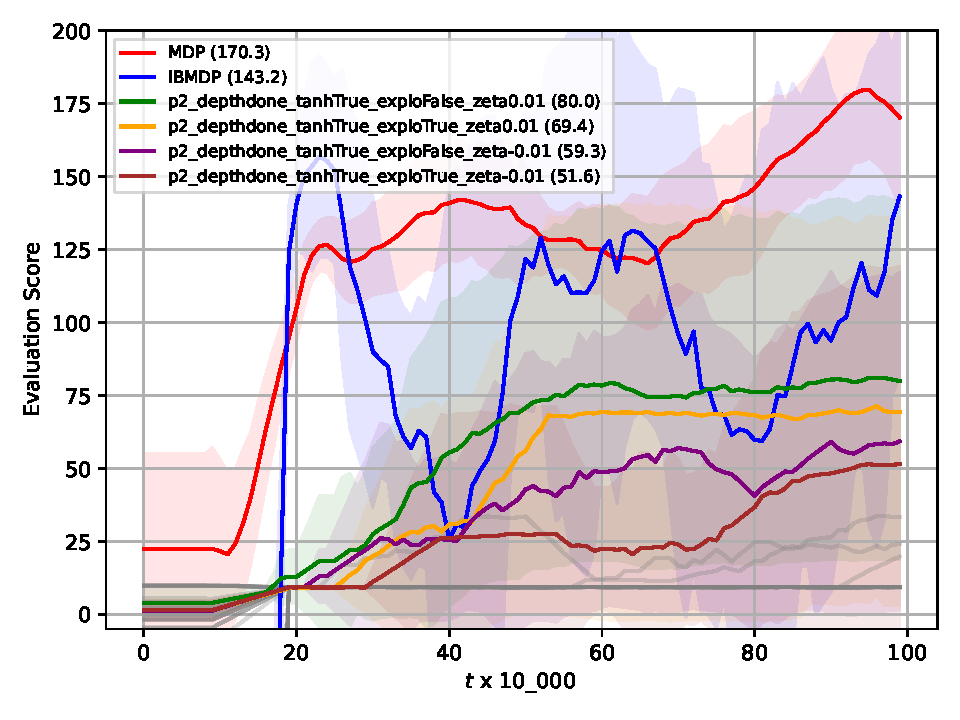
\includegraphics[width=0.7\textwidth]{images/images_part1/dqn.pdf}
    \caption{Variations of modified DQN and DQN (cf.~\ref{tab:ibmdp-rl1}), on different CartPole IBMDPs (cf. ~\ref{tab:ibmdp-params}). We give different line-styles for the learning curves for DQN applied directly on CartPole and DQN applied on the IBMDP.
    Since there are multiple possible candidates for the original paper hyperparameters, we choose to color the (modified DQN variant, IBMDP variant) pair that resulted in the best decision tree policy on CartPole among the instances that could match the original paper's.
    Shaded areas represent the confidence interval at 95\% at each measure on the y-axis.}
\end{figure}\label{fig:res-dqn}

\begin{figure}
    \centering
    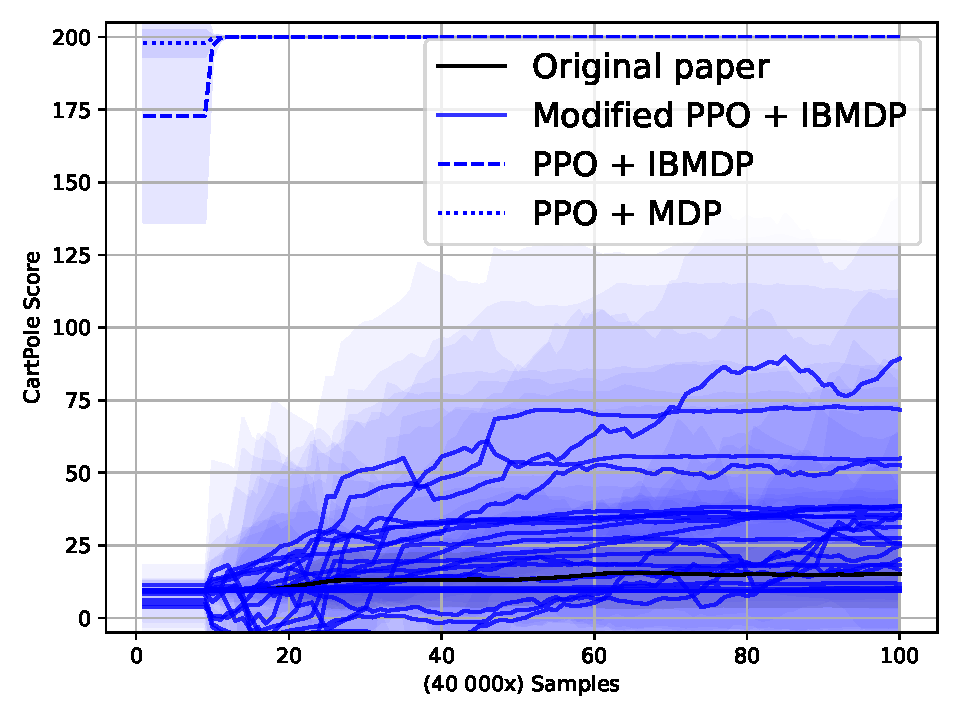
\includegraphics[width=0.7\textwidth]{images/images_part1/ppo.pdf}
    \caption{Variations of modified PPO and PPO (cf.~\ref{tab:ibmdp-rl2}), on different CartPole IBMDPs (cf. ~\ref{tab:ibmdp-params}). We give different line-styles for the learning curves for PPO applied directly on CartPole and DQN applied on the IBMDP.
    Since there are multiple possible candidates for the original paper hyperparameters, we choose to color the (modified PPO variant, IBMDP variant) pair that resulted in the best decision tree policy on CartPole among the instances that could match the original paper's.
    Shaded areas represent the confidence interval at 95\% at each measure on the y-axis.}
\end{figure}\label{fig:res-ppo}

On Figure~\ref{fig:res-dqn}, we observe that modified DQN can learn in IBMDPs--the curves have an increasing trend--but we also observe that modified DQN finds poor decision tree policies for CartPole in average--the curves flatten at the end of the x-axis and have low y-values--.
In particular, among all the learning curves that could possibly correspond to the original paper's modified DQN, the learning curve with highest final y-value is converging to decision tree policies for CartPole high poor performances.

On Figure~\ref{fig:res-ppo}, we observe that modified PPO finds decision tree policies with almost 150 cumulative rewards towards the end of training. The performance difference with modified DQN could be because we trained longer, like in the original paper.

However it could also be because DQN-like algorithm with those hyperparameters struggle to learn in CartPole (IB)MDPs.
Indeed, we notice that for DQN-like baselines, learning seems difficult in general independently of the setting.

On Figures~\ref{fig:res-dqn} and~\ref{fig:res-ppo}, we observe that standard RL baselines (RL + IBMDP and RL + MDP), learn better CartPole policies in average than their modified counterparts that learn partially observable policies (\ref{def:po-policy}). 
On Figure~\ref{fig:res-ppo}, it is clear that for the standard PPO baselines, learning is super efficient and algorithms learn optimal policies with reward 200 in few thousands steps.

In Tables ~\ref{tab:mod-dqn} and~\ref{tab:mod-ppo} we report the top-5 hyperparameters for Modified RL baselines when learning partially observable IBMDP policies in terms of extracted decision tree policies performances in CartPole control.
\begin{table}[h]
    \centering
    \caption{Top 5 Hyperparameter Configurations for modified DQN + IBMDP, bold font represent the original paper hyperparameters.}\label{tab:mod-dqn}
    \label{tab:top5_results}
    \begin{tabular}{ccccccS}
    \toprule
    Rank & $p$ & Depth control & Activation & Exploration & $\zeta$ & {Final Performance} \\
    \midrule
    1 & 3 & termination & $\operatorname{tanh}()$ & 0.9 & 0.01 & 53 \\
    2 & 2 & termination & $\operatorname{tanh}()$ & 0.5 & -0.01 & 24 \\
    \textbf{3} & \textbf{3} & \textbf{termination} & $\operatorname{tanh}()$ & \textbf{0.5} & \textbf{-0.01} & \textbf{24} \\
    4 & 2 & termination & $\operatorname{tanh}()$ & 0.5 & 0.01 & 23 \\
    5 & 2 & termination & $\operatorname{tanh}()$ & 0.9 & -0.01 & 22 \\
    \bottomrule
    \end{tabular}
    \end{table}

    \begin{table}[h]
        \centering
        \caption{Top 5 Hyperparameter Configurations for modified PPO + IBMDP, bold font represent the original paper hyperparameters.}\label{tab:mod-ppo}
        \label{tab:top5_ppo_results}
        \begin{tabular}{cccccS}
        \toprule
        Rank & $p$ & Depth Control & Activation & $\zeta$ & {Final Performance} \\
        \midrule
        1 & 3 & reward & $\operatorname{relu}()$ & 0.01 & 139 \\
        2 & 3 & done & $\operatorname{relu}()$ & 0.01 & 132 \\
        \textbf{3} & \textbf{3} & \textbf{reward} & $\operatorname{tanh}()$ & \textbf{-0.01} & \textbf{119} \\
        4 & 3 & reward & $\operatorname{relu}()$ & -0.01 & 117 \\
        5 & 3 & reward & $\operatorname{tanh}()$ & 0.01 & 116 \\
        \bottomrule
        \end{tabular}
        \end{table}


\subsection{What decision tree policies does direct reinforcement learning return for CartPole?}

\begin{figure}
    \centering
    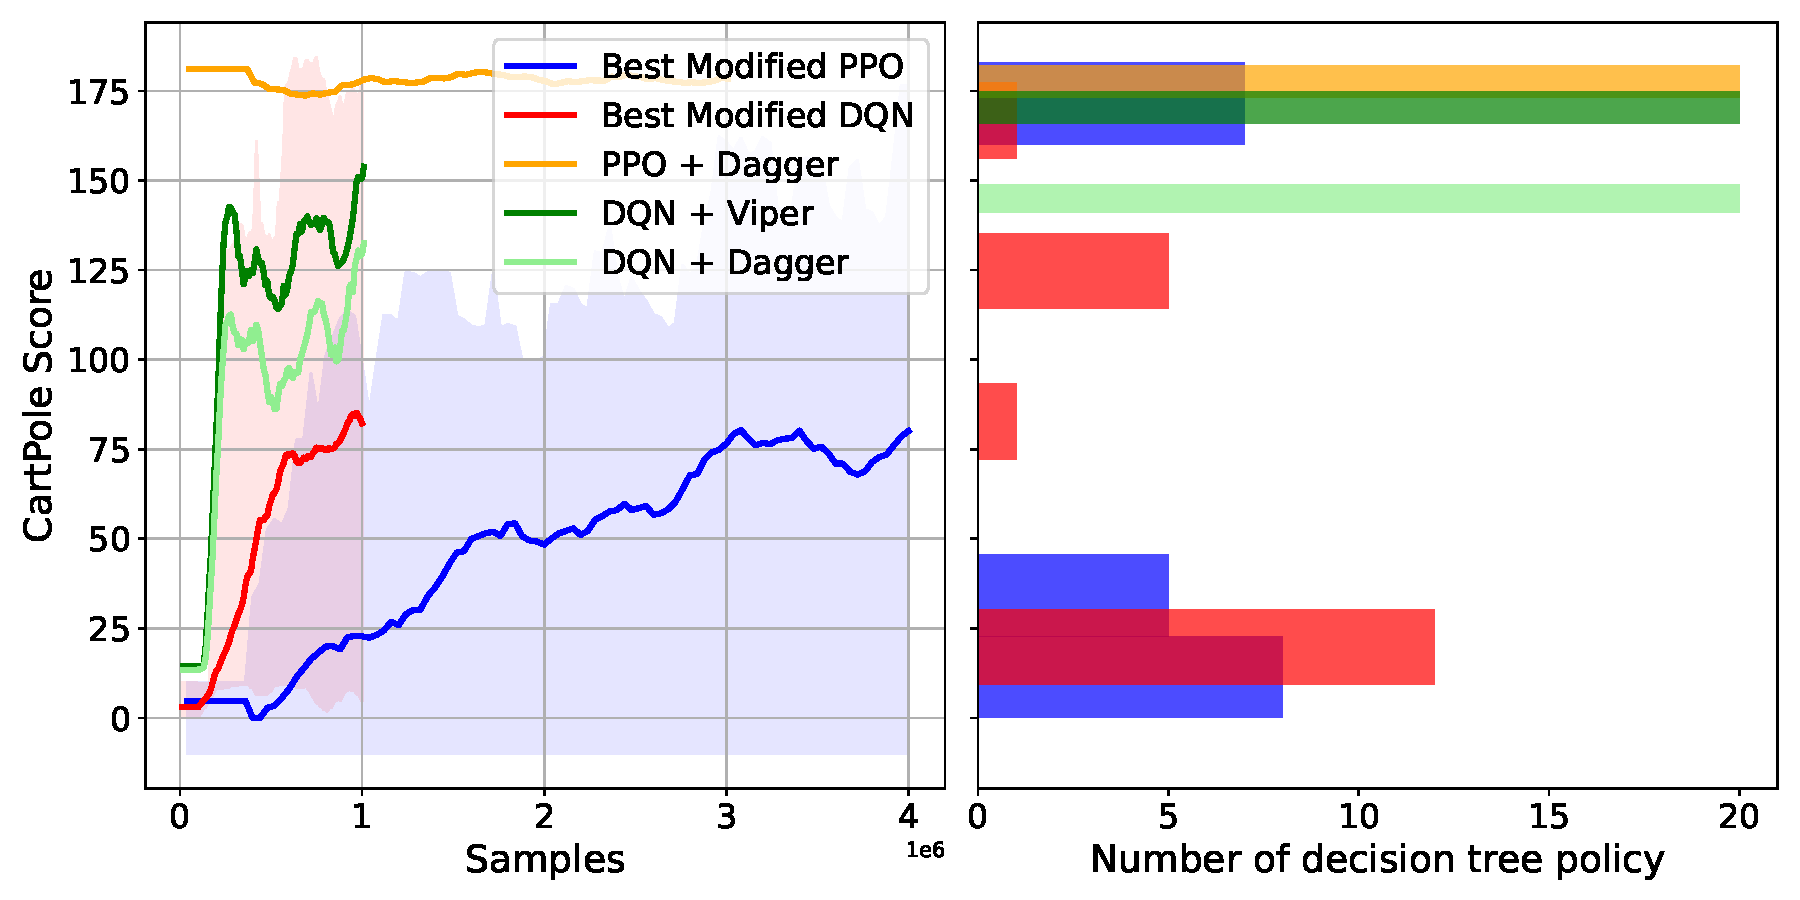
\includegraphics[width=1\textwidth]{images/images_part1/ppo_tree_study.pdf}
    \caption{(left) Mean performance of the best--w.r.t. to the RL objective (~\ref{def:mdp-obj}) for CartPole--modified RL + IBMDP combination. Shaded areas representing the min and max performance over the 20 seeds during training. (right) Corresponding scores distribution of the final decision tree policies performances w.r.t. to the RL objective (~\ref{def:mdp-obj}) for CartPole.}\label{fig:ppo-trees}
\end{figure}


\begin{figure}[htbp]
    \centering
    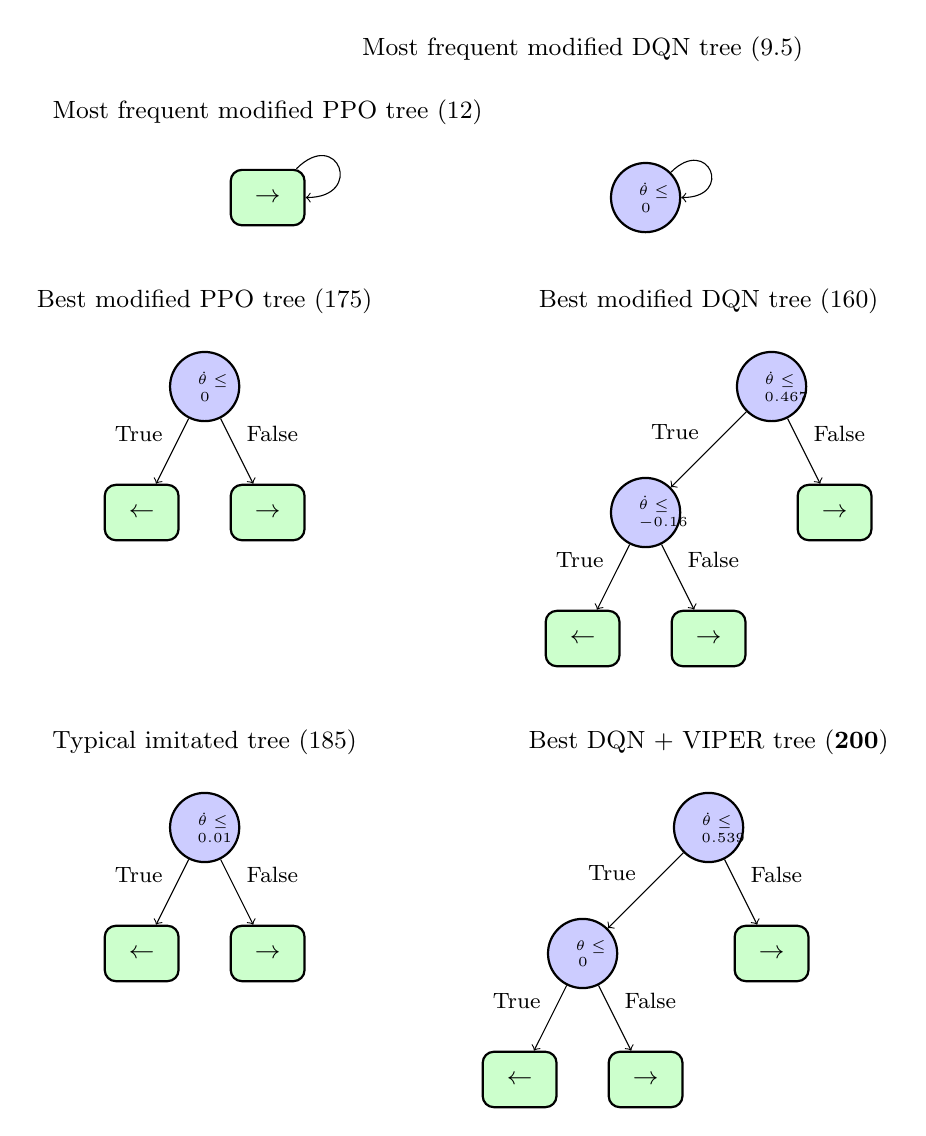
\begin{tikzpicture}[
        scale=0.8,
        decision/.style={circle, draw, thick, fill=blue!20, text width=0.5em, text centered, minimum height=2.5em, font=\tiny},
        leaf/.style={rectangle, draw, thick, fill=green!20, text width=2em, text centered, rounded corners, minimum height=2em, font=\small},
        edge_label/.style={font=\footnotesize, midway}
    ]

        \node[leaf] (tree7_root) at (-2,3) {$\rightarrow$};
        \draw[->] (tree7_root) to[out=45,in=0,looseness=5] (tree7_root);

        \node[decision] (tree7_root) at (4,3) {$\dot{\theta} \leq 0$};
        \draw[->] (tree7_root) to[out=45,in=0,looseness=5] (tree7_root);
        
        % Tree 4: if x <= 0.5 move right else move left
        \node[decision] (tree4_root) at (-3,0) { $\dot{\theta}\leq 0$};
        \node[leaf] (tree4_right) at (-4,-2) {$\leftarrow$};
        \node[leaf] (tree4_left) at (-2,-2) {$\rightarrow$};
        \draw[->] (tree4_root) -- (tree4_right) node[edge_label, above left] {True};
        \draw[->] (tree4_root) -- (tree4_left) node[edge_label, above right] {False};
        

        % Tree 7: if x <= 0.5 and y <= 0.5 move right else move down
        \node[decision] (tree7_root) at (6,0) {$\dot{\theta}\leq 0.467$};
        \node[decision] (tree7_y) at (4,-2) {$\dot{\theta}\leq -0.16$};
        \node[leaf] (tree7_right) at (3,-4) {$\leftarrow$};
        \node[leaf] (tree7_down) at (5,-4) {$\rightarrow$};
        \node[leaf] (tree7_down2) at (7,-2) {$\rightarrow$};
        \draw[->] (tree7_root) -- (tree7_y) node[edge_label, above left] {True};
        \draw[->] (tree7_root) -- (tree7_down2) node[edge_label, above right] {False};
        \draw[->] (tree7_y) -- (tree7_right) node[edge_label, above left] {True};
        \draw[->] (tree7_y) -- (tree7_down) node[edge_label, above right] {False};




        % Tree 4: if x <= 0.5 move right else move left (Second row, left)
        \node[decision] (tree4_root2) at (-3,-7) { $\dot{\theta}\leq 0.01$};
        \node[leaf] (tree4_right2) at (-4,-9) {$\leftarrow$};
        \node[leaf] (tree4_left2) at (-2,-9) {$\rightarrow$};
        \draw[->] (tree4_root2) -- (tree4_right2) node[edge_label, above left] {True};
        \draw[->] (tree4_root2) -- (tree4_left2) node[edge_label, above right] {False};


        % Tree 7: if x <= 0.5 and y <= 0.5 move right else move down (Second row, right)
        \node[decision] (tree7_root2) at (5,-7) {$\dot{\theta}\leq 0.539$};
        \node[decision] (tree7_y2) at (3,-9) {$\theta\leq 0$};
        \node[leaf] (tree7_right2) at (2,-11) {$\leftarrow$};
        \node[leaf] (tree7_down3) at (4,-11) {$\rightarrow$};
        \node[leaf] (tree7_down4) at (6,-9) {$\rightarrow$};
        \draw[->] (tree7_root2) -- (tree7_y2) node[edge_label, above left] {True};
        \draw[->] (tree7_root2) -- (tree7_down4) node[edge_label, above right] {False};
        \draw[->] (tree7_y2) -- (tree7_right2) node[edge_label, above left] {True};
        \draw[->] (tree7_y2) -- (tree7_down3) node[edge_label, above right] {False};
        

        % Labels
        \node[above] at (-2,4) {{\small Most frequent modified PPO tree (12)}};
        \node[above] at (3,5) {{\small Most frequent modified DQN tree (9.5)}};

        \node[above] at (-3,1) {{\small Best modified PPO tree (175)}};
        \node[above] at (5,1) {{\small Best modified DQN tree (160)}};
        \node[above] at (-3,-6) {{\small Typical imitated tree (185)}};
        \node[above] at (5,-6) {{\small Best DQN + VIPER tree (\textbf{200})}};


    \end{tikzpicture}
    \caption{Trees obtained by Deep RL in IBMDPs against trees obtained with imitation (CartPole cumulative rewards). $\theta$ and $\dot{\theta}$ are respectively the angle and the angular velocity of the pole}
    \label{fig:trees-drl}
\end{figure}


On Figure~\ref{fig:ppo-trees}, we isolate the best performing algorithms instantiations that learn decision tree policies for CartPole.
We compare the best modified DQN or modified PPO to imitation learning baselines that use the surrogate imitation objective (~\ref{def:il}) to find CartPole decision tree policies.
We find that despite having poor performances in \textit{average}, the modified deep reinforcement learning baselines can find very good decision tree policies as shown by the min-max shaded areas on the left of Figure~\ref{fig:ppo-trees} and the corresponding estimated density of final trees performances.
However this is not desirable, a user typically wants an algorithm that can consistently find good decision tree policies.
As shown by the estimated densities, indirect methods consistently find good decision tree policies (the higher modes of distributions are on the right of the plot).
On the other hand, the final trees returned by direct RL methods seem equally distributed on both extremes of the scores.

On Figure~\ref{fig:trees-drl}, we present the best decision tree policies for CartPole returned by modified DQN and modified PPO.
We used Algorithm~\ref{alg:extract-tree} to extract 20 trees from the 20 partially observable policies returned by the modified deep reinforcement learning algorithms over the 20 training seeds.
We then plot the best tree for each baseline.
Those trees get an average reward of roughly 175.
Similarly, we plot a representative tree for imitation learning baseline as well as a tree that is optimal for CartPole w.r.t. (~\ref{def:mdp-obj}) obtained with VIPER. 
Unlike for direct methods, the trees returned by imitation learning are extremely similar across seeds. In particular they often only vary in the scalar value used in the root node but in general have the same structure and test the angular velocity.
On the other hand the most frequent trees across seeds returned by modified RL baselines are ``trivial'' decision tree policy that either repeat the same base action forever or repeat the same IGA (Def. ~\ref{def:ibmdp}) forever.


\section{Discussion}
We have shown that compared to learning non-interpretable neural network policies for the base MDP or some associated IBMDP, reinforcement learning of partially observable policies in IBMDP is less efficient (cf. Figures~\ref{fig:res-dqn} and~\ref{fig:res-ppo}). 
As a consequence, only a handful of modified RL runs are able to learn decision tree policies that are on par with imitated trees (cf. Figure~\ref{fig:ppo-trees}).

In the next chapter, we highlight the connections between direct interpretable RL (Def.~\ref{def:irl}) and POMDPs to get insights on the hardness of direct reinforcement learning of decision trees.
%
% Troisième chapitre
\chapter{Conclusion}
\section{What happens when the MDP's transitions are independent of the current state?}


%
%
% Deuxième partie éventuelle
\part{An easier problem: Learning Decision Trees for MDPs that are Classification tasks}
%
% Quatrième chapitre
\chapter{Introduction}\label{sec:part2}\footnote{This work was published at the 31st ACM SIGKDD conference in 2025:\url{https://dl.acm.org/doi/10.1145/3711896.3736868}}
In this part of the manuscript we design a novel decision tree induction algorithm for supervised learning (\ref{def:sl}) using the MDP formalism.
There already exist works formulating the decision tree induction problem as solving a Markov decision process~\cite{Dulac_Arnold_2011,garlapati2015reinforcementlearningapproachonline,topin2021iterative,chaouki2024branchesfastdynamicprogramming}.
In particular, we showed in the previous part how Topin et al.~\cite{topin2021iterative} could be used to do that using classification POIBMDPs (cf. section~\ref{sec:pomdp-classif}).
We move away from classification POIBMDPs and use a novel MDP formulation that we detail later.
The key differences compared to, e.g.~\cite{topin2021iterative} is that our MDP states are sets of training data rather than feature bounds (cf. definition~\ref{def:cpoibmdp}) and that we dynamically define the set of information gathering actions (cf. definition~\ref{def:ibmdp}).
One other novelty, is that unlike existing works that use reinforcement learning (section~\ref{sec:rl}), we use dynamic programming~\cite{Bellman} to solve exactly decision tree induction formulated as an MDP.

This part of the manuscript is organized as follows.
In this chapter, we motivate the need for new decision tree induction algorithms and present the related works.
In chapter~\ref{sec:dt-mdp}, we introduce a novel MDP formulation of decision tree induction.
Finally, in chapter~\ref{sec:exps-dt}, we show that our new decision tree induction framework performs very well both in terms of training loss and generalization capabilites.

\subsection{Why do we want new decision tree induction algorithms?}
In supervised learning (~\ref{def:sl}), decision trees (\ref{fig:dt}) are valued for their interpretability and performance. 
While greedy decision tree algorithms like CART (algorithm~\ref{alg:cart} \cite{breiman1984classification}remain widely used due to their computational efficiency, they often produce sub-optimal solutions with respect to a regularized training loss (\ref{def:sl}). 
Conversely, optimal decision tree methods can find better solutions but are computationally intensive and typically limited to shallow trees or binary features. We present Dynamic Programming Decision Trees (DPDT), a framework that bridges the gap between greedy and optimal approaches. 
DPDT relies on a Markov decision process (\ref{def:mdp}) formulation combined with heuristic split generation to construct near-optimal decision trees with significantly reduced computational complexity. 
Our approach dynamically limits the set of admissible splits at each node while directly optimizing the tree regularized training loss. Theoretical analysis demonstrates that DPDT can minimize regularized training losses at least as well as CART\@. 
Our empirical study shows on multiple datasets that DPDT achieves near-optimal loss with orders of magnitude fewer operations than existing optimal solvers. 
More importantly, extensive benchmarking suggests statistically significant improvements of DPDT over both CART and optimal decision trees in terms of generalization to unseen data. We demonstrate DPDT practicality through applications to boosting, where it consistently outperforms baselines. 
Our framework provides a promising direction for developing efficient, near-optimal decision tree algorithms that scale to practical applications.

\begin{figure}
    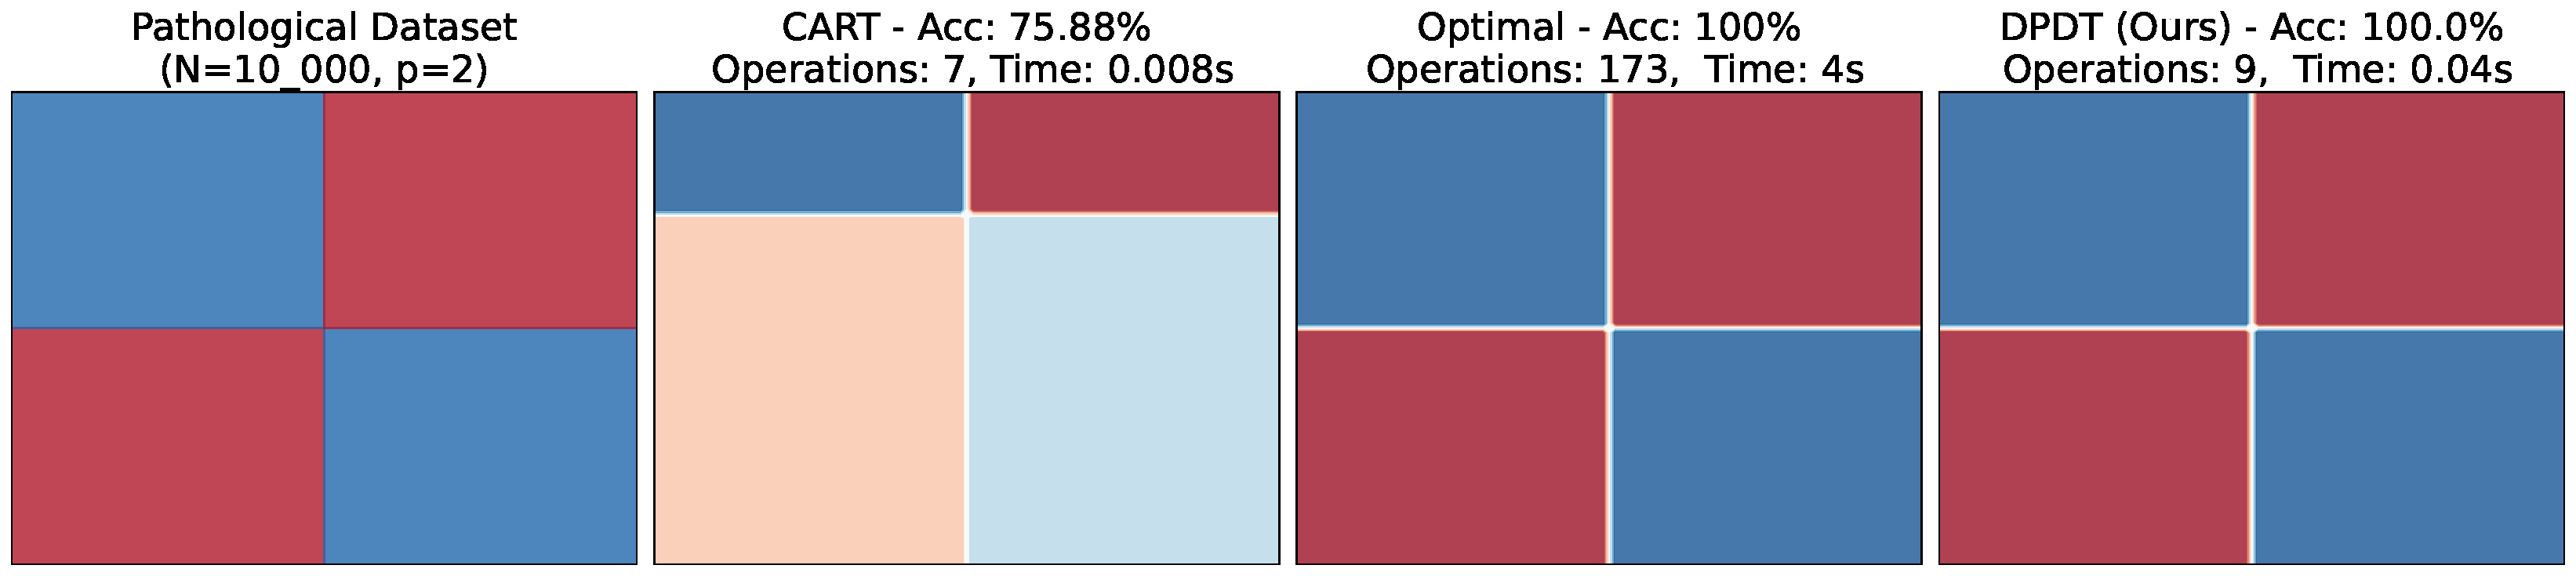
\includegraphics[width=\textwidth]{images/figures/patho_bounds_comparison_checkers.pdf}
    \caption{Pathological dataset and learned depth-2 trees with their scores, complexities, runtimes, and decision boundaries.}
    \label{fig:patho}
\end{figure}

We already saw in the Introduction (\ref{sec:dt}) that decision trees are well studied in supervised learning.
Decision tree inductions algorithms~\cite{ID3,c45,breiman1984classification} are at the core of various machine learning applications. 
Ensembles of decision trees such as tree boosting~\cite{stcohFriedman,FriedmanBoosting,xgb,10.5555/3327757.3327770} are the state-of-the-art for supervised learning on tabular data \cite{grinsztajn2022tree}.

To motivate the design of new decision tree induction algorithms, figure~\ref{fig:patho} exhibits a dataset for which existing greedy algorithms are suboptimal, and optimal algorithms are computationally expensive. 
The dataset is made up of $N=10^4$ samples in $p=2$ dimensions that can be perfectly labeled with a decision tree of depth 2. When running CART, greedily choosing the root node yields a suboptimal tree.
This is because greedy algorithms compute locally optimal splits in terms of information gain. In our example, the greedy splits always give two children datasets which themselves need depth-2 trees to be perfectly split.
On the other hand, to find the root node, an optimal algorithm such as \cite{quantbnb} iterates over all possible splits, that is, $N\times p={20,000}$ operations to find one node of the solution tree.

In this work, we present a framework for designing non-greedy decision tree induction algorithms that optimize a regularized training loss nearly as well as optimal methods. This is achieved with orders of magnitude less operations, and hence dramatic computation savings.
We call this framework ``Dynamic Programming Decision Trees'' (DPDT). For every node, DPDT heuristically and dynamically limits the set of admissible splits to a few good candidates. Then, DPDT optimizes the regularized training loss with some depth constraints.
Theoretically, we show that DPDT minimizes the empirical risk at least as well as CART\@.
Empirically, we show that on all tested datasets, DPDT can reach 99\% of the optimal regularized train accuracy while using thousands times less operations than current optimal solvers. 
More importantly, we follow \cite{grinsztajn2022tree} methodology to benchmark DPDT against both CART and optimal trees on hard datasets. Following the same methodology, we compare boosted DPDT \cite{FREUND1997119} to boosted CART and to some deep learning methods and show clear superiority of DPDT.

\section{Related work}

To learn decision trees, greedy approaches like CART (algorithm~\ref{alg:cart} \cite{breiman1984classification}) iteratively partition the training dataset by taking splits optimizing a local objective such as the Gini impurity or the entropy. 
This makes CART suboptimal with respect to training losses (\ref{def:sl}) \cite{Murthy}. 
But CART remains the default decision tree algorithm in many machine learning libraries such as \cite{scikit-learn,xgb,ke2017lightgbm,9533597} because it can scale to very deep trees and is very fast.
To avoid overfitting, greedy trees are learned with a maximal depth or pruned a posteriori \cite[chapter 3]{breiman1984classification}. 
In recent years, more complex optimal decision tree induction algorithms have shown consistent gains over CART in terms of generalization capabilities \cite{oct,verwer2017learning,murtree}.

Optimal decision tree approaches optimize a regularized training loss while using a minimal number of splits~\cite{oct,mfoct,binoct,quantbnb,murtree,blossom,pystreed,chaouki2024branchesfastdynamicprogramming}.
However, direct optimization is not a convenient approach, as finding the optimal tree is known to be NP-Hard \cite{npcomplete}. Despite the large number of algorithmic tricks to make optimal decision tree solvers efficient~\cite{murtree,quantbnb}, their complexity scales with the number of samples and the maximum depth constraint.
Furthermore, optimal decision tree induction algorithms are usually constrained to binary-features dataset while CART can deal with any type of feature. When optimal decision tree algorithms deal with continuous features, they can usually learn only shallow trees, e.g. Quant-BnB \cite{quantbnb} can only compute optimal trees up to depth 3.
\texttt{PySTreeD}, the latest optimal decision tree library~\cite{pystreed}, can compute decision trees with depths larger than three but uses heuristics to binarize a dataset with continuous features during a pre-processing step. % following for example the Minimum Description Length Principle \cite{MDL}. 
Despite their limitations to binary features and their huge computational complexities, encouraging practical results for optimal trees have been obtained \cite{how-eff,lin2020generalized,costa2023recent,vanderlinden2024optimalgreedydecisiontrees}.
Among others, they show that optimal methods under the same depth constraint (up to depth four) find
trees with 1--2\% greater test accuracy than greedy methods.

In this part, we only consider the induction of non-parametric (cf. section~\ref{related-work-pomdp}) binary depth-constrained axis-aligned trees. 
We write this model class $\mathcal{T}_D$ where $D$ is the maximum tree depth.
Axis-aligned tree nodes only test one data feature only against one thresholds only as opposed to e.g. oblique trees~\cite{murthy1994system}.
In our definition (\ref{sec:dt}), this means that we only consider Boolean functions $(j, \mathbb{R}):\rightarrow \{0, 1\}$ (the careful reader might notice the clear similarity with information gathering actions in IBMDPs (definition~\ref{def:ibmdp},~\cite{topin2021iterative})).
Like for the reinforcement learning setting, there exists a line of work on parametric trees: Tree Alternating Optimization (TAO) algorithm~\cite{NEURIPS2018_185c29dc,9534446,10.1145/3412815.3416882} that only optimizes tree nodes threshold values for fixed nodes features similarly to optimizing neural network weights with gradient-based methods. 

Now we write explicitely the supervised learning objective (\ref{def:sl}) for decision trees:

\begin{definition}[Supervised learning of decision trees (decision tree induction)]\label{eq:suplearning}
    Assume that we have access to a set of $N$ examples denoted $\mathcal{E} = {\{(x_i, y_i)\}}_{i=1}^N$. Each datum $x_i$ is described by a set of $p$ features. $y_i \in {\mathcal Y}$ is the label associated with $x_i$. The objective of decision tree induction is to find a tree with maximum depth $D$, $T \in \mathcal{T}_D$ that minimizes:
    \begin{align*}
        {\mathcal L}_\alpha(T) = \frac{1}{N}\overset{N}{\underset{i=1}{\sum}}{l}(y_i, T(x_i)) + \alpha C(T) \\
\end{align*}
where $C: \mathcal{T}_D \rightarrow \mathbb{R}$ is a complexity penalty that helps prevent or reduce overfitting such as the number of nodes~\cite{breiman1984classification,quantbnb}, or the expected number of splits to label a data\cite{how-eff}. The complexity penalty is weighted by $\alpha \in [0, 1]$. %For regression problems where $\mathcal{Y} \subset \mathbb R$, we use the squared error $l(y_i, T(x_i)) = {(y_i - T(x_i))}^2$. 
\end{definition}

In the rest of this part we focus on classification tasks: we use the 0--1 loss $l(y_i, T(x_i)) = 1_{\{y_i\neq T(x_i)\}}$.
Please note while we focus on classification tasks, our framework extends naturally to regression tasks.

In the supervised learning setting, there exist many other areas of decision tree research \cite{loh2014fifty} such as inducing non-axis parallel decision trees \cite{murthy1994system,10.1145/3637528.3671903}, splitting criteria of greedy trees \cite{vanderlinden2024optimalgreedydecisiontrees}, different optimization of parametric trees \cite{NIPS2015_1579779b,10.5555/3327757.3327770}, or pruning methods \cite{pruning1,pruning2}. 
%
% Cinquième chapitre
\chapter{Decision tree induction as solving an MDP}\label{sec:dt-mdp}

\section{The Markov decision process}\label{sec:the-mdp}
We now formulate the decision tree induction problem (cf. definition~\ref{eq:suplearning}) as finding the optimal policy in an MDP (cf. definition~\ref{def:mdp-obj}).

Given a set of examples $\mathcal{E}$, the induction of a decision tree is made of a sequence of decisions: at each node, we must decide whether it is better to split (a subset of) $\mathcal{E}$, or %assign a class label and 
to create a leaf node.

This sequential decision-making process corresponds to an MDP $\mathcal{M} \langle S, A, R_{\alpha}, T, T_0 \rangle$ (cf. definition~\ref{def:mdp}) that we present next.
%The state space $S$ consists of pairs $(X,d)$ where $X \subseteq \mathcal{E}$, and $d \in \{0,\ldots,D\}$ is the current depth in the tree. Formally $S = \{ (X, d) \in P(\mathcal{E}) \times \{0, \ldots, D\} \}$ where $P(\mathcal{E})$ denotes the power set of $\mathcal{E}$.
A state is a pair made of a subset of examples $\mathcal{X}\subseteq\mathcal E$ and a depth $d$.
Like for classification POIBMDPs (cf. definition~\ref{def:ibmdp} and algorithm~\ref{alg:extract-tree}), the depth $d$ is actually not necessary to extract a tree from a policy.
However, it is necessary in order to solve the MDP.
Indeed, because we constrain the model class to limited-depth trees, the horizon of our MDP is finite and hence as per~\cite{puterman}, the optimal policy is non-Markovian and depends on the time.

The set of states is $S = \{ (\mathcal{X}, d) \in P(\mathcal{E}) \times \{0, \ldots, D\} \}$ where $P(\mathcal{E})$ denotes the power set of $\mathcal{E}$. $d \in \{0,\ldots,D\}$ is the current depth in the tree.
An action $A$ consists in creating either a split node, or a leaf node (label assignment). We denote the set of candidate split nodes $ {\mathcal F} $. A split node in $\mathcal F$ is a pair made of one feature $i$ and a threshold value $x_{ij}\in \mathcal{E}$.
So, we can write $A = {\mathcal{F} \cup \{ 1, \ldots, K \}}$ (these are essentially information gathering actions).
From state $s=(X,d)$ and a splitting action $a \in {\mathcal F}$, the transition function $P$ moves to the next state $s_l = (\mathcal{X}_l, d+1)$ with probability $p_l = \frac{|\mathcal{X}_l|}{|\mathcal{X}|}$ where $\mathcal{X}_l = \{(\boldsymbol{x}_i, y_i) \in \mathcal{X}: \boldsymbol{x}_i \leq x_{ij}\}$, or to state $s_r = (\mathcal{X} \setminus \mathcal{X}_l, d+1)$ with probability $1-p_l$. For a class assignment action $a \in \{1,\ldots,K\}$, the chain reaches an absorbing terminal state with probability 1. 
The reward function $R_{\alpha}: S \times A \rightarrow \mathbb{R}$ returns $-\alpha$ for splitting actions (this is $\zeta$ in a classification POIBMDP (cf. definition~\ref{def:cpoibmdp})) and the proportion of misclassified examples of $\mathcal{X}$ $-\frac{1}{|\mathcal{X}|}\sum_{(\boldsymbol{x}_i,y_i) \in \mathcal{X}} l(y_i, a)$ for class assignment actions. $\alpha \in [0,1]$ controls the accuracy-complexity trade-off defined in the regularized training objective \ref{eq:suplearning}. 

The solution to this MDP is a deterministic policy $\pi: S \rightarrow A$ that maximizes {$J_{\alpha}(\pi) ={\mathbb{E}}\left[\sum_{t = 0}^D R_{\alpha}(s_t, \pi(s_t))\right]$\label{def:finite-mdp-obj}}, the expected sum of rewards where the expectation is taken over transitions $s_{t+1}\sim P(s_t, \pi(s_t))$ starting from initial state $s_0 = (\mathcal{E}, 0)$.
This objective is a re-writing of the RL objective (cf. definition~\ref{def:mdp-obj}) where the trajectory have finite lengths $D$ rather than being infinite.
Any such policy can be converted into a binary decision tree through a recursive extraction function $E(\pi, s)$ (equivalent to algorithm~\ref{alg:extract-tree}) that returns, either a leaf node with class $\pi(s)$ if $\pi(s)$ is a class assignment, or a tree with root node containing split $\pi(s)$ and left/right sub-trees $E(\pi, s_l)$/$E(\pi, s_r)$ if $\pi(s)$ is a split. The final decision tree $T$ is obtained by calling $E(\pi, s_0)$ on the initial state $s_0$. 

\begin{proposition}[Objective Equivalence]\label{prop:equiv}
Let $\pi$ be a deterministic policy of the MDP (cf. section~\ref{sec:the-mdp}) and $\pi^*$ be an optimal deterministic policy. 
Then $J_\alpha(\pi) = -{\mathcal L}_\alpha(E(\pi, s_0))$ and $T^* = E(\pi^*, s_0)$ where $T^*$ is a tree that optimizes the decision tree induction objective (cf. definition~\ref{eq:suplearning}).
\end{proposition}
This proposition is key as it states that the return of any policy of the MDP defined above is equal to the regularized training accuracy of the tree extracted from this policy.
A consequence of this proposition is that when all possible splits are considered, the optimal policy will generate the optimal tree w.r.t the decision tree induction objective.

\begin{proof}
For the purpose of the proof, we overload the definition of $J_\alpha$ and $\mathcal L_\alpha$, to make explicit the dependency on the dataset and the maximum depth. 
As such, $J_\alpha(\pi)$ becomes $J_\alpha(\pi, {\mathcal E}, D)$ and ${\mathcal L}_\alpha(T)$ becomes ${\mathcal L}_\alpha(T, {\mathcal E})$. 
Let us first show that the relation $J_\alpha(\pi, {\mathcal E}, 0) = -{\mathcal L}_\alpha(T, {\mathcal E})$ is true. 
If the maximum depth is $D = 0$ then $\pi(s_0)$ is necessarily a class assignment, in which case the expected number of splits is zero and the relation is obviously true since the reward is the opposite of the average classification loss. 
Now assume it is true for any dataset and tree of depth at most $D$ with $D \geq 0$ and let us prove that it holds for all trees of depth $D + 1$. 
For a tree $T$ of depth $D + 1$ the root is necessarily a split node. Let $T_l = E(\pi, s_l)$ and $T_r = E(\pi, s_r)$ be the left and right sub-trees of the root node of $T$. 
Since both sub-trees are of depth at most $D$, the relation holds and we have $J_\alpha(\pi, \mathcal{X}_l, D) = {\mathcal L}_\alpha(T_l, \mathcal{X}_l)$ and $J_\alpha(\pi, \mathcal{X}_r, D) = {\mathcal L}_\alpha(T_r, \mathcal{X}_r)$, where $\mathcal{X}_l$ and $\mathcal{X}_r$ are the datasets of the ``right'' and ``left'' states to which the MDP transitions---with probabilities $p_l$ and $p_r$---upon application of $\pi(s_0)$ in $s_0$, as described in the MDP formulation. 
Moreover, from the definition of the policy return we have 
\begin{align*}
   J_\alpha(&\pi, {\mathcal E}, D + 1) = -\alpha + p_l * J_\alpha(\pi, \mathcal{X}_l, D) + p_r * J_\alpha(\pi, \mathcal{X}_r, D)\\
   &= -\alpha - p_l * {\mathcal L}_\alpha(T_l, \mathcal{X}_l) - p_r * {\mathcal L}_\alpha(T_r, D)\\
   &= -\alpha - p_l * \Bigg(\frac{1}{|\mathcal{X}_l|}\sum_{(\boldsymbol{x}_i, y_i)\in \mathcal{X}_l}l(y_i, T_l(\boldsymbol{x}_i))  + \alpha C(T_l)\Bigg)\\
   &\ - p_r * \Bigg(\frac{1}{|\mathcal{X}_r|}\sum_{(\boldsymbol{x}_i, y_i)\in \mathcal{X}_r}l(y_i, T_r(\boldsymbol{x}_i))  + \alpha C(T_r)\Bigg)\\
   &= -\frac{1}{N}\sum_{(\boldsymbol{x}_i, y_i)\in \mathcal{X}}l(y_i, T(\boldsymbol{x}_i)) - \alpha (1 + p_l C(T_l) + p_r C(T_r))\\
   &= -{\mathcal L}(T, {\mathcal E}) 
\end{align*}
\end{proof}

\section{Algorithm}\label{sec:dpdt}

We now present the Dynamic Programming Decision Tree (DPDT) induction algorithm. 
The algorithm consists of two essential steps. The first and most computationally expensive step constructs the MDP presented in section~\ref{sec:the-mdp}. 
The second step solves it to obtain a policy that maximizes the objective from definition~\ref{def:finite-mdp-obj} and that is equivalent to a decision tree. Both steps are now detailed.

\subsection{Constructing the MDP}

An algorithm constructing the MDP of section~\ref{sec:the-mdp} essentially computes the set of all possible decision trees of maximum depth $D$ which decision nodes are in $\mathcal F$. 
The transition function of this specific MDP is a directed acyclic graph. Each node of this graph corresponds to a state for which one computes the transition and reward functions. 
%% PP : je comment-out ce qui suit qui est un detail d'implantation qui ne change rien à la complexité de l'algorithme. Il faut le dire plus loin ; d'ailleurs il en est aussi déjà question en 4.3.
%To limit memory usage of non-terminal nodes, instead of storing all the samples in $(\mathcal{X},d)$, we only store $d$ and the binary vector of size $N$, $x_{bin} = {(1_{\{\boldsymbol{x}_i \in \mathcal{X}\}})}_{i\in \{1,\ldots,N\}}$. 
%Even then,
Considering all possible splits in $\mathcal F$ does not scale.
We thus introduce a state-dependent action space $A_s$, much smaller than $A$ and populated by a splits generating function. In figure \ref{fig:schema-mdp}, we illustrate the MDP constructed for the classification of a toy dataset using some arbitrary splitting function.

\begin{figure}
      \centering
      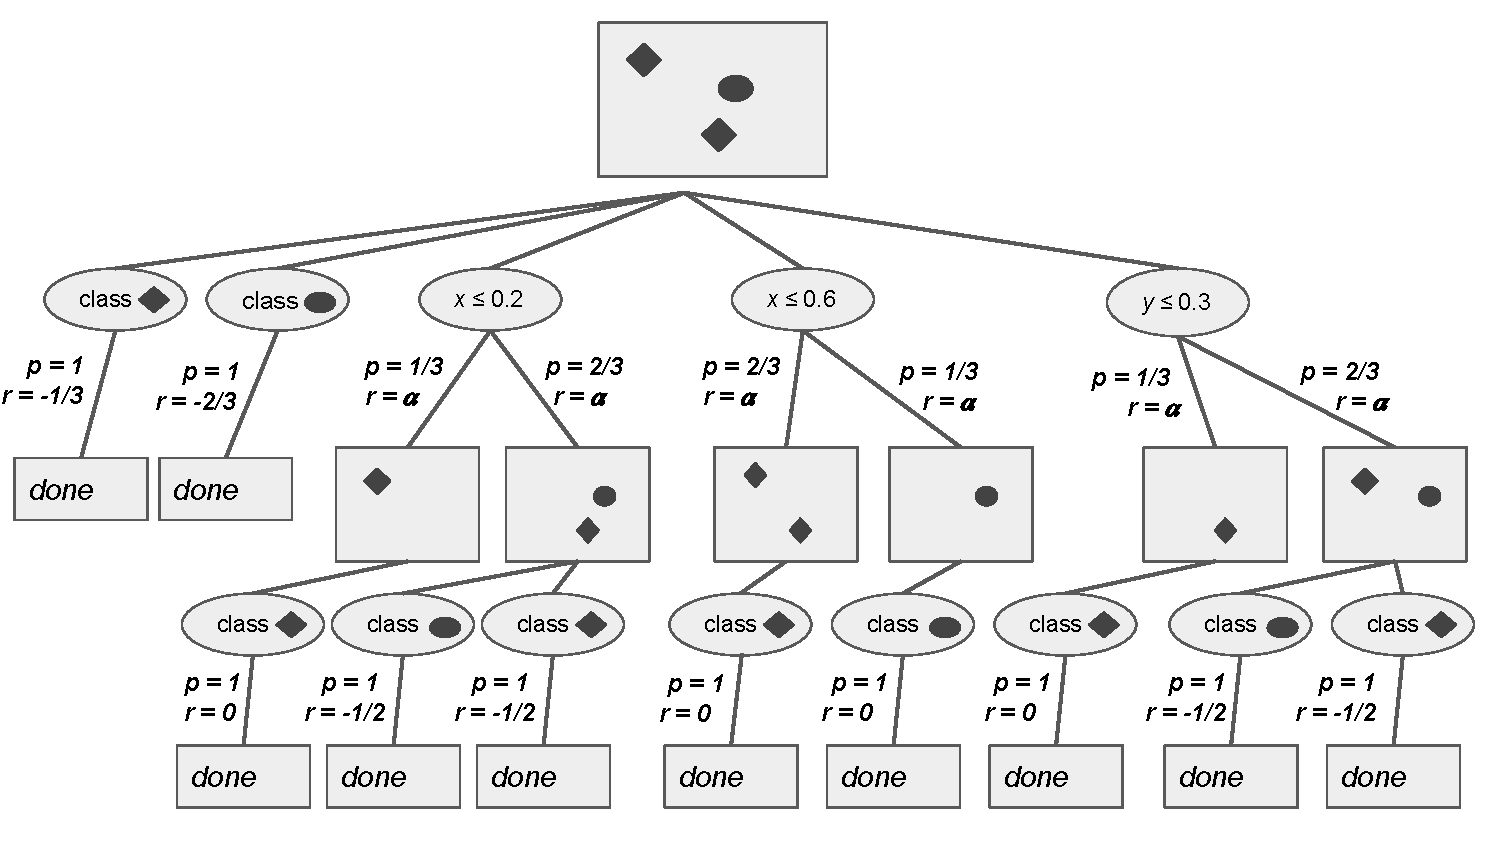
\includegraphics[width=0.9\linewidth]{images/figures/schema_mdp.pdf}
      \caption{Schematics of the MDP from section~\ref{sec:the-mdp} to learn a decision tree of depth 2 to classify a toy dataset with three samples, two features (x,y), and two classes (oval, diamond) and using an arbitrary splits generating function.}\label{fig:schema-mdp}
      \end{figure}

\subsection{Heuristic splits generating functions}\label{sec:testgen}

A split generating function is any function $\phi$ that maps an MDP state, i.e., a subset of training examples, to a split node. It has the form $\phi: S \rightarrow P(\mathcal{F})$, where $P(\mathcal{F})$ is the power set of all possible split nodes in $\mathcal F$. 
For a state $s \in S$, the state-dependent action space is defined by $A_s = \phi(s) \cup  \{1,\ldots,K\}$. 

When the split generating function does not return all the possible candidate split nodes given a state, solving the MDP with state-dependent actions $A_s$ is not guaranteed to yield the minimizing tree for the decision tree induction problem (cf. definition~\ref{eq:suplearning}), as the 
optimization is then performed on the subset of trees of depth smaller or equal to $D$, $\mathcal{T}_D$. 
We now define some interesting split generating functions and provide the time complexity of the associated decision tree algorithms. The time complexity is given in big-O of the number of candidate split nodes considered during computations. 
% Building a depth-1 greedy tree hides a time complexity of $O(np\log(np))$ to sort the splits by information gains \cite{breiman1984classification}.
%%%>>>>>>> c90c7909bd5d3b8cfee3901e21a456980dfd72e1

\paragraph{Exhaustive function} When $\mathcal{F} \subseteq \phi(s), \forall s \in S$, the MDP contains all possible splits of a certain set of examples. In this case, \textit{the optimal MDP policy is the optimal decision tree of depth at most D},
and the number of states of the MDP would be $O({(2Np)}^D)$. Solving the MDP for $A_s = \phi(s)$ is equivalent to running one of the optimal tree induction algorithms~\cite{verwer2017learning,oct,pystreed,quantbnb,binoct,murtree,mfoct,blossom,lin2020generalized,chaouki2024branchesfastdynamicprogramming}.

\paragraph{Top $B$ most informative splits}\label{topk-heuristic}~\cite{topk} proposed to generate splits with a function that returns, for any state $s=(\mathcal{X},d)$, the $B$ most informative splits over $\mathcal{X}$ with respect to some information gain measure such as the entropy or the Gini impurity. 
The number of states in the MDP would be $O({(2B)}^D)$. \textit{When $B=1$, the optimal policy of the MDP is the greedy tree.} 
In practice, we noticed that the returned set of splits lacked diversity and often consists of splits on the same feature with minor changes to the threshold value. 

% PP : don't know why mais ci-dessous, si on met un '.' après {CART}, le pdf en affiche 2. Si on n'en met pas, on en voit un !
\paragraph{Calls to CART}\label{cart-heuristic} Instead of returning the most informative split at each state $s=(\mathcal{X},d)$, we propose to find the most discriminative split, i.e.\@ the feature splits that best predicts the class of data in $\mathcal{X}$.
We can do this by considering the split nodes of the greedy tree. In practice, we run CART on $s$ and use the returned nodes as $\phi(s)$. We control the number of MDP states by constraining CART trees with a maximum number of nodes $B$: $\phi(s) = nodes(\text{CART}(s, max\_nodes=B))$
The number of MDP states would be $O({(2B)}^D)$.\textit{When $B=1$, the MDP policy corresponds to the greedy tree.} The process of generating split nodes with calls to CART is illustrated in figure \ref{fig:schema-dpdt}.

\begin{figure}
      \centering
      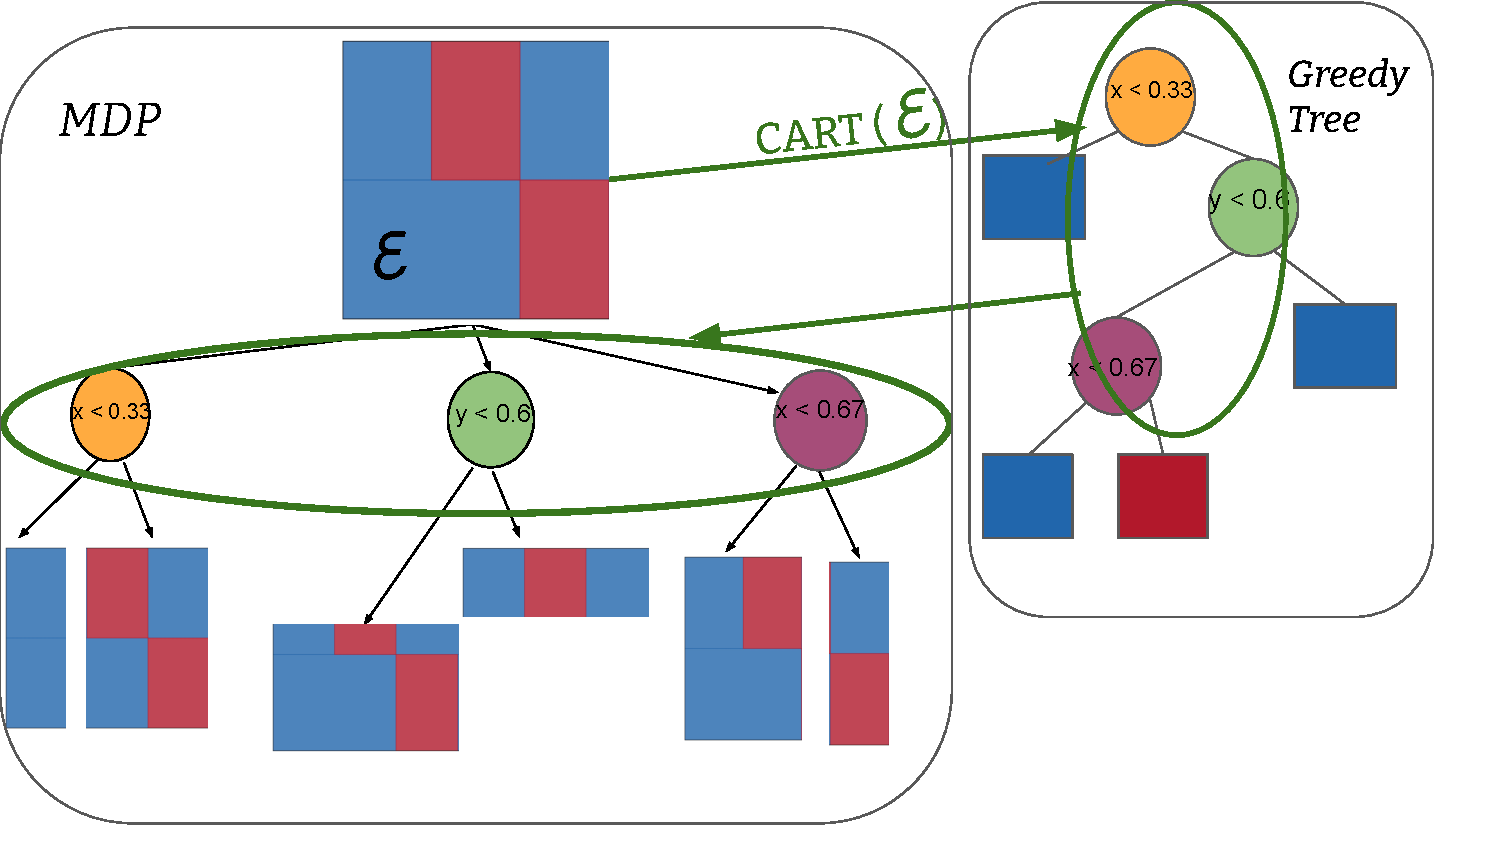
\includegraphics[trim={0 0cm 0 0},clip,width=0.9\textwidth]{images/figures/schematic_cart_node_select.pdf}
      \caption{How CART is used in DPDT to generate candidate splits given the example data in the current state.}\label{fig:schema-dpdt}
\end{figure}



\subsection{Dynamic programming to solve the MDP}
\RestyleAlgo{ruled}
\SetKwComment{Comment}{}{}
        \begin{algorithm}
            \KwData{$\text{Dataset }\mathcal{E}, \text{max depth }D, \text{split function }\phi(), $\\
            $\text{split function parameter } B,  \text{regularizing term }\alpha$}
            \KwResult{$\text{Tree } T$}
            $\mathcal{M} \gets build\_mdp(\mathcal{E}, D, \phi(), B)$\label{line:build_mdp} \\
            \Comment{{// Backward induction}}
            $Q^*(s,a) \gets R_{\alpha}^{\mathcal{M}}(s,a) + \sum_{s'} P^{\mathcal{M}}(s,a,s') \max_{a' \in A_{s'}^{\mathcal{M}}} Q^*(s',a') \forall s,a \in \mathcal{M}$\\
            \Comment{{// Get the optimal policy}}
            $\pi^*(s) = \operatorname{argmax}_{a \in A_s^{\mathcal{M}}} Q^*(s, a) \forall s \in \mathcal{M} $\\
            \Comment{{// Extracting tree from policy}}
            $T \gets E(\pi^*,s_0^{\mathcal{M}}) $
            \caption{DPDT}\label{alg:dpdt}
        \end{algorithm}
        
After constructing the MDP with a chosen splits generating function, we solve for the optimal policy using dynamic programming. Starting from terminal states and working backward to the initial state, we compute the optimal state-action values using Bellman's optimality equation~\cite{Bellman}, and then deducing the optimal policy.

From now on, we write DPDT to denote algorithm \ref{alg:dpdt} when the split function is a call to CART. We discuss key bottlenecks when implementing DPDT in subsequent sections. We now state theoretical results when using DPDT with the CART heuristic. 

\subsection{Performance guarantees for DPDT}
We now show that: 1) DPDT minimizes the loss from decision tree induction objective (cf. definition~\ref{eq:suplearning}) at least as well as greedy trees and 2) there exists problems for which DPDT has strictly lower loss than greedy trees. 
As we restrict the action space at a given state $s$ to a subset of all possible split nodes, DPDT is not guaranteed to find the tree minimizing Eq. \ref{eq:suplearning}. However, we are still guaranteed to find trees that are better or equivalent to those induced by CART:
\begin{theorem}[MDP solutions are not worse than the greedy tree]\label{prop:cart}
Let $\pi^*$ be an optimal deterministic policy of the MDP, where the action space at every state is restricted to the top $B$ most informative or discriminative splits. 
Let $T_0$ be the tree induced by CART and $\{T_1,\dots,T_M\}$ all the sub-trees of $T_0$, \footnote{These sub-trees are interesting to consider since they can be returned by common postprocessing operations following a call to CART, that prune some of the nodes from $T_0$. Please see \cite{pruning1} for a review of pruning methods for decision trees.} then for any $\alpha > 0$, 
\[
{\mathcal L}_\alpha(E(\pi^*, s_0)) \leq \min_{0\leq i\leq M}{\mathcal L}_\alpha(T_i)
\]
\end{theorem}

\begin{proof}
Let us first define $C(T)$, the expected number of splits performed by tree $T$ on dataset $\mathcal E$. 
Here $T$ is deduced from policy $\pi$, i.e. $T=E(\pi, s_0)$. $C(T)$ can be defined recursively as $C(T) = 0$ if $T$ is a leaf node, and $C(T) = 1 + p_l C(T_l) + p_r  C(T_r)$, where $T_l = E(\pi, s_l)$ and $T_r = E(\pi, s_r)$. 
In words, when the root of $T$ is a split node, the expected number of splits is one plus the expected number of splits of the left and right sub-trees of the root node.
\end{proof}

It is known that the greedy tree of depth 2 fails to perfectly classify the XOR problem as shown in figure \ref{fig:patho} and in \cite{Murthy,how-eff}. We aim to show that DPDT is a cheap way to alleviate the weaknesses of greedy trees in this type of problems. The following theorem states that there exist classification problems such that DPDT optimizes the regularized training loss strictly better than greedy algorithms such as CART, ID3 or C4.5.
\begin{theorem}[DPDT can be strictly better than greedy]\label{thm:better_greedy}
There exists a dataset and a depth $D$ such that the DPDT tree $T^{DPDT}_D$ is strictly better than the greedy tree $T^{greedy}_{D}$ , i.e, $\mathcal{L}_{\alpha=0}(T^{greedy}_{D}) > \mathcal{L}_{\alpha=0}(T^{DPDT}_{D})$.
\end{theorem}

The proof of this theorem is given in the next section.

\subsection{Proof of improvement over CART}\label{proof-improve-opt}
In this section we construct a dataset for which the greedy tree of depth 2 fails to accurately classify data while DPDT with calls to CART as a splits generating function guarantees a strictly better accuracy. The dataset is the XOR pattern like in figure \ref{fig:patho}. We will first show that greedy tree induction like CART chooses the first split at random and the second split in between the two columns or rows. Then we will quantify the misclassification of the depth-2 greedy tree on the XOR gate. Finally we will show that using the second greedy split as the root of a tree and then building the remaining nodes greedily, i.e. running DPDT with the CART heuristic, strictly decreases the misclassification. 
\begin{definition}[XOR dataset]\label{def:checkerboard}
     Let us defined the XOR dataset as $\mathcal{E}_{XOR} = \{(\boldsymbol{x}_i, y_i)\}_{i=1}^N$. $\boldsymbol{x}_i = (\boldsymbol{x}_i, y_i) \sim \mathcal{U}([0,1]^2)$ are i.i.d 2-features samples. $y_i = f(\boldsymbol{x}_i)$ are alternating classes with $f(x,y) = (\lfloor 2x \rfloor + \lfloor 2y \rfloor) \bmod 2$.
\end{definition}

\begin{lemma} The first greedy split is chosen at random on the XOR dataset from definition \ref{def:checkerboard}.
\end{lemma}\label{lem:first-split}
\begin{proof}
Let us consider an arbitrary split $x = x_v$ parallel to the y-axis. The results apply to splits parallel to the x-axis because the XOR pattern is the same when rotated 90 degrees. The split $x_v$ partitions the dataset into two regions $R_{left}$ and $R_{right}$. Since the dataset has two columns and two rows, any rectangular area that spans the whole height $[0,1)$ has the same proportion of class 0 samples and class 1 samples from definition \ref{def:checkerboard}. So in both $R_{left}$ and $R_{right}$ the probabilities of observing class 0 or class 1 at random are $\frac{1}{2}$. Since the class distributions in left and right regions are independent of the split location, all splits have the same objective value when the objective is a measure of information gain like the entropy or the Gini impurity. Hence, the first split in a greedily induced tree is chosen at random.
\end{proof}

\begin{lemma}\label{lem:second-split}
    When the first split is greedy on the XOR dataset from definition \ref{def:checkerboard}, the second greedy splits are chosen perpendicular to the first split at $y=\frac{1}{2}$
\end{lemma}

\begin{proof}
Assume without loss of generality due to symmetries, that the first greedy split is vertical, at \(x=x_v\), with $x_v <= \frac{1}{2}$. This split partitions the unit square into
$R_{left} = [0,x_v)\times[0,1)$ and $R_{right} = [x_v,1)\times[0,1)$. The split $y=\frac{1}{2}$ further partitions $R_{left}$ into $R_{left-down}$ and $R_{left-up}$ with same areas $x_v \times y = \frac{x_v}{2}$. Due to the XOR pattern, there are only samples of class 0 in $R_{left-down}$ and only samples of class 1 in $R_{left-up}$. Hence the the split $y = \frac{1}{2}$ maximizes the information gain in $R_{left}$, hence the second greedy split given an arbitrary first split $x=x_v$ is necessarily $y=\frac{1}{2}$.
\end{proof}
\begin{definition}[Forced- Tree]\label{def:grid-tree}
Let us define the forced-tree as a greedy tree that is forced to make its first split at $y=\frac{1}{2}$.
\end{definition}

\begin{lemma}\label{lem:dpdt-better}
The forced-tree of depth 2 has a 0 loss on the XOR dataset from definition \ref{def:checkerboard} while, with probability $1-\frac{1}{|\mathcal{E}_{XOR}|}$, the greedy tree of depth 2 has strictly positive loss. 
\end{lemma}

\begin{proof}
This is trivial from the definition of the forced tree since if we start with the split $y=\frac{1}{2}$, then clearly CART will correctly split the remaining data. If instead the first split is some  $x_v \neq \frac{1}{2}$ then CART is bound to make an error with only one extra split allowed. Since the first split is chosen at random, from Lemma \ref{lem:first-split}, there are only two splits ($x=\frac{1}{2}$ and $y=\frac{1}{2}$) out of $2 |\mathcal{E}_{XOR}|$ that do not lead to sub-optimality.   
\end{proof}
We can now formally prove theorem \ref{thm:better_greedy}.
\begin{proof}
    By definition of DPDT, all instances of DPDT with the CART nodes parameter $B\geq2$ include the forced-tree from definition \ref{def:grid-tree} in their solution set when applied to the XOR dataset (definition \ref{def:checkerboard}). 
    We know from lemma \ref{lem:dpdt-better} that with high probability, the forced-tree of depth 2 is strictly more accurate than the greedy tree of depth 2 on the XOR dataset. Because we know by proposition \ref{prop:equiv} that DPDT returns the tree with maximal accuracy from its solution set, we can say that DPDT depth-2 trees are strictly better than depth-2 greedy trees returned by e.g. CART on the XOR dataset. 
\end{proof}

\subsection{Practical implementation}

The key bottlenecks lie in the MDP construction step of DPDT (section \ref{sec:the-mdp}). In nature, all decision tree induction algorithms have time complexity exponential in the number of training subsets per tree depth $D$: $O((2B)^D)$, e.g., CART has $O(2^D)$ time complexity. We already saw that DPDT saves time by not considering all possible tree splits but only $B$ of them. Using state-dependent split generation also allows to generate more or less candidates at different depths of the tree. Indeed, the MDP state $s = (\mathcal{X},d)$ contains the current depth during the MDP construction process. This means that one can control DPDT's time complexity by giving multiple values of maximum nodes: given $(B_1, B_2, ..., B_D)$, the splits generating function in algorithm~\ref{alg:dpdt} becomes $\phi(s_i) = \phi(\boldsymbol{x}_i, d=1) = nodes(\text{CART}(s, max\_nodes=B_1))$ and  $\phi(s_j) = \phi(\mathcal{X}_j, d=2) = nodes(\text{CART}(s, max\_nodes=B_2))$.

Similarly, the space complexity of DPDT is exponential in the space required to store training examples $\mathcal E$. Indeed, the MDP states that DPDT builds in algorithm~\ref{alg:dpdt} are training samples $\mathcal X \subseteq \mathcal E$. Hence, the total space required to run DPDT is $O({Np}(2B)^{D})$ where $Np$ is the size of $\mathcal{E}$. In practice, one should implement DPDT in a depth first search manner to obtain a space complexity linear in the size of training set: $O(DNp)$. In practice DPDT builds the MDP from section~\ref{sec:the-mdp} by starting from the root and recursively splitting the training set while backpropagating the $Q$-values. This is possible because the MDP we solve has a (not necessarily binary) tree structure (see figure~\ref{fig:schema-mdp}) and because the $Q$-values of a state only depend on future states. 

We implemented DPDT\footnote{\url{https://github.com/KohlerHECTOR/DPDTreeEstimator}} following scikit-learn API~\cite{sklearn_api} with depth-first search and state-depth-dependent splits generating.
In the next chapter, we evaluate DPDT using the above implementation.
%
% Sixième chapitre
\chapter{Dynamic programming decision trees in practice}\label{sec:exps-dt}

In this section, we empirically demonstrate strong properties of DPDT trees. 
The first part of our experiments focuses on the quality of solutions obtained by DPDT for objective Eq.\ref{eq:suplearning} compared to greedy and optimal trees. We know by theorems \ref{prop:cart} and \ref{thm:better_greedy} that DPDT trees should find better solutions than greedy algorithms for certain problems; but what about real problems?
After showing that DPDT can find optimal trees by considering much less solutions and thus performing orders of magnitude less operations, we will study the generalization capabilities of the latter: do DPDT trees label unseen data accurately?

\section{DPDT optimizing capabilities}
\begin{table}[ht]
    \centering
    \tiny
    \caption{Comparison of train accuracies of depth-3 trees and number of operations on classification tasks. For DPDT and Top-B, ``light'' configurations have split function parameters (8, 1, 1) ``full'' have parameters (8, 8, 8). We also include the mean train accuracy over 5 deep RL runs. \textbf{Bold} values are optimal accuracies and {\color{blue} blue} values are the largest non-optimal accuracies.}
    \label{tab:tree_comparison_combined}
    \begin{tabular}{l|cc||cc|cc|cc|c||cc|cc|cc}
    \toprule
    & & & \multicolumn{7}{c||}{\textbf{Accuracy}} & \multicolumn{6}{c}{\textbf{Operations}}\\
    \midrule
    & & & Opt & Greedy & \multicolumn{2}{c|}{DPDT} & \multicolumn{2}{c|}{Top-B} & \multicolumn{1}{c||}{Deep RL} & Opt & Greedy & \multicolumn{2}{c|}{DPDT} & \multicolumn{2}{c}{Top-B}\\
    \textbf{Dataset} & N & p & Quant-BnB & CART & light & full & light & full & Modified DQN & Quant-BnB & CART & light & full & light & full \\
    % version précédente rempplacée par les 3 lignes ci-dessus :
    % & & & \multicolumn{2}{c|}{\textbf{Accuracy}} & \multicolumn{2}{c|}{DPDT} & \multicolumn{2}{c|}{Top-B} & \multicolumn{1}{c||}{Deep RL} & \multicolumn{2}{c|}{\textbf{Operations}} & \multicolumn{2}{c|}{DPDT} & \multicolumn{2}{c}{Top-B}\\
    % \textbf{Dataset} & N & p & Opt & Greedy & light & full & light & full & Custard & Opt & Greedy & light & full & light & full \\
    \midrule
    room & 8103 & 16 & \textbf{0.992} & 0.968 & \color{blue} 0.991 & \textbf{0.992} & 0.990 & \textbf{0.992} & 0.715 &$10^6$ & 15 & 286 & 16100 & 111 & 16100 \\
    bean & 10888 & 16  & \textbf{0.871} & 0.777 & 0.812 & \color{blue} 0.853 & 0.804 & 0.841 & 0.182 & 5$\cdot 10^6$ & 15 & 295 & 25900 & 112 & 16800 \\
    eeg & 11984 & 14  & \textbf{0.708} & 0.666 & 0.689 & \color{blue} 0.706 & 0.684 & 0.699 & 0.549 & 2$\cdot 10^6$ & 13 & 289 & 26000 & 95 & 11000 \\
    avila & 10430 & 10  & \textbf{0.585} & 0.532 & \color{blue}0.574 & \textbf{0.585} & 0.563 & 0.572 & 0.409 & 3$\cdot 10^7$ & 9 & 268 & 24700 & 60 & 38900 \\
    magic & 15216 & 10 & \textbf{0.831} & 0.801 & 0.822 & \color{blue} 0.828 & 0.807 & 0.816 & 0.581 &6$\cdot 10^6$ & 15 & 298 & 28000 & 70 & 4190 \\
    htru & 14318 & 8  & \textbf{0.981} & 0.979 & 0.979 & \color{blue}0.980 & 0.979 & \color{blue}0.980 & 0.860 & 6$\cdot 10^7$ & 15 & 295 & 25300 & 55 & 2180 \\
    occup. & 8143 & 5 & \textbf{0.994} & 0.989 & 0.991 & \textbf{0.994} & 0.990 & \color{blue}0.992 & 0.647 & 7$\cdot 10^5$ & 13 & 280 & 16300 & 33 & 510 \\
    skin & 196045 & 3 & \textbf{0.969} & \color{blue}0.966 & \color{blue}0.966 & \color{blue}0.966 & \color{blue}0.966 & \color{blue}0.966 & 0.612 & 7$\cdot 10^4$ & 15 & 301 & 23300 & 20 & 126 \\
    fault & 1552 & 27 & \textbf{0.682} & 0.553 & 0.672 & \color{blue}0.674 & 0.672 & 0.673 & 0.303 & 9$\cdot 10^8$ & 13 & 295 & 24200 & 111 & 16800 \\
    segment & 1848 & 18 & \textbf{0.887} & 0.574 & 0.812 & \color{blue}0.879 & 0.786 & 0.825 & 0.137 & 2$\cdot 10^6$ & 7 & 220 & 16300 & 68 & 11400 \\
    page & 4378 & 10 &  \textbf{0.971} & 0.964 & \color{blue}0.970 & \color{blue}0.970 & 0.964 & 0.965 & 0.902 &$10^7$ & 15 & 298 & 22400 & 701 & 4050 \\
    bidding & 5056 & 9  & \textbf{0.993} & 0.981 & \color{blue}0.985 & \textbf{0.993} & 0.985 & \textbf{0.993} & 0.810 & 3$\cdot 10^5$ & 13 & 256 & 9360 & 58 & 2700 \\
    raisin & 720 & 7 & \textbf{0.894} & 0.869 & 0.879 & \color{blue}0.886 & 0.875 & 0.883 & 0.509 & 4$\cdot 10^6$ & 15 & 295 & 20900 & 48 & 1440 \\
    rice & 3048 & 7 & \textbf{0.938} & 0.933 & 0.934 & \color{blue}0.937 & 0.933 & 0.936 & 0.519 & 2$\cdot 10^7$ & 15 & 298 & 25500 & 49 & 1470 \\
    wilt & 4339 & 5 & \textbf{0.996} & 0.993 & 0.994 & \color{blue}0.995 & 0.994 & 0.994 & 0.984 &3$\cdot 10^5$ & 13 & 274 & 11300 & 33 & 465 \\
    bank & 1097 & 4 & \textbf{0.983} & 0.933 & 0.971 & \color{blue}0.980 & 0.951 & 0.974 & 0.496 & 6$\cdot 10^4$ & 13 & 271 & 7990 & 26 & 256 \\
% ancienne présentation :
    %% room & 8103 & 16 & 0.992 & 0.968 & 0.991 & 0.992 & 0.990 & 0.992 & 0.715 & 1.34e+06 & 15 & 286 & 16100 & 111 & 16100 \\
    %% bean & 10888 & 16  & 0.871 & 0.777 & 0.812 & 0.853 & 0.804 & 0.841 & 0.182 & 4.66e+06 & 15 & 295 & 25900 & 112 & 16800 \\
    %% eeg & 11984 & 14  & 0.708 & 0.666 & 0.689 & 0.706 & 0.684 & 0.699 & 0.549 & 1.50e+08 & 13 & 289 & 26000 & 95 & 11000 \\
    %% avila & 10430 & 10  & 0.585 & 0.532 & 0.574 & 0.585 & 0.563 & 0.572 & 0.409 & 2.70e+07 & 9 & 268 & 24700 & 60 & 38900 \\
    %% magic & 15216 & 10 & 0.831 & 0.801 & 0.822 & 0.828 & 0.807 & 0.816 & 0.581 &5.71e+06 & 15 & 298 & 28000 & 70 & 4190 \\
    %% htru & 14318 & 8  & 0.981 & 0.979 & 0.979 & 0.980 & 0.979 & 0.980 & 0.860 & 6.22e+07 & 15 & 295 & 25300 & 55 & 2180 \\
    %% occupancy & 8143 & 5 & 0.994 & 0.989 & 0.991 & 0.994 & 0.990 & 0.992 & 0.647 & 6.81e+05 & 13 & 280 & 16300 & 33 & 510 \\
    %% skin & 196045 & 3 & 0.969 & 0.966 & 0.966 & 0.966 & 0.966 & 0.966 & 0.612 & 71100 & 15 & 301 & 23300 & 20 & 126 \\
    %% fault & 1552 & 27 & 0.682 & 0.553 & 0.672 & 0.674 & 0.672 & 0.673 & 0.303 & 9.32e+08 & 13 & 295 & 24200 & 111 & 16800 \\
    %% segment & 1848 & 18 & 0.887 & 0.574 & 0.812 & 0.879 & 0.786 & 0.825 & 0.137 & 2.13e+06 & 7 & 220 & 16300 & 68 & 11400 \\
    %% page & 4378 & 10 &  0.971 & 0.964 & 0.970 & 0.970 & 0.964 & 0.965 & 0.902 & 9.62e+06 & 15 & 298 & 22400 & 701 & 4050 \\
    %% bidding & 5056 & 9  & 0.993 & 0.981 & 0.985 & 0.993 & 0.985 & 0.993 & 0.810 & 2.69e+05 & 13 & 256 & 9360 & 58 & 2700 \\
    %% raisin & 720 & 7 & 0.894 & 0.869 & 0.879 & 0.886 & 0.875 & 0.883 & 0.509 & 3.98e+06 & 15 & 295 & 20900 & 48 & 1440 \\
    %% rice & 3048 & 7 & 0.938 & 0.933 & 0.934 & 0.937 & 0.933 & 0.936 & 0.519 & 2.08e+07 & 15 & 298 & 25500 & 49 & 1470 \\
    %% wilt & 4339 & 5 & 0.996 & 0.993 & 0.994 & 0.995 & 0.994 & 0.994 & 0.984 &3.20e+05 & 13 & 274 & 11300 & 33 & 465 \\
    %% bank & 1097 & 4 & 0.983 & 0.933 & 0.971 & 0.980 & 0.951 & 0.974 & 0.496 & 62500 & 13 & 271 & 7990 & 26 & 256 \\
    \bottomrule
    \end{tabular}
\end{table}
\begin{figure}
    \centering
    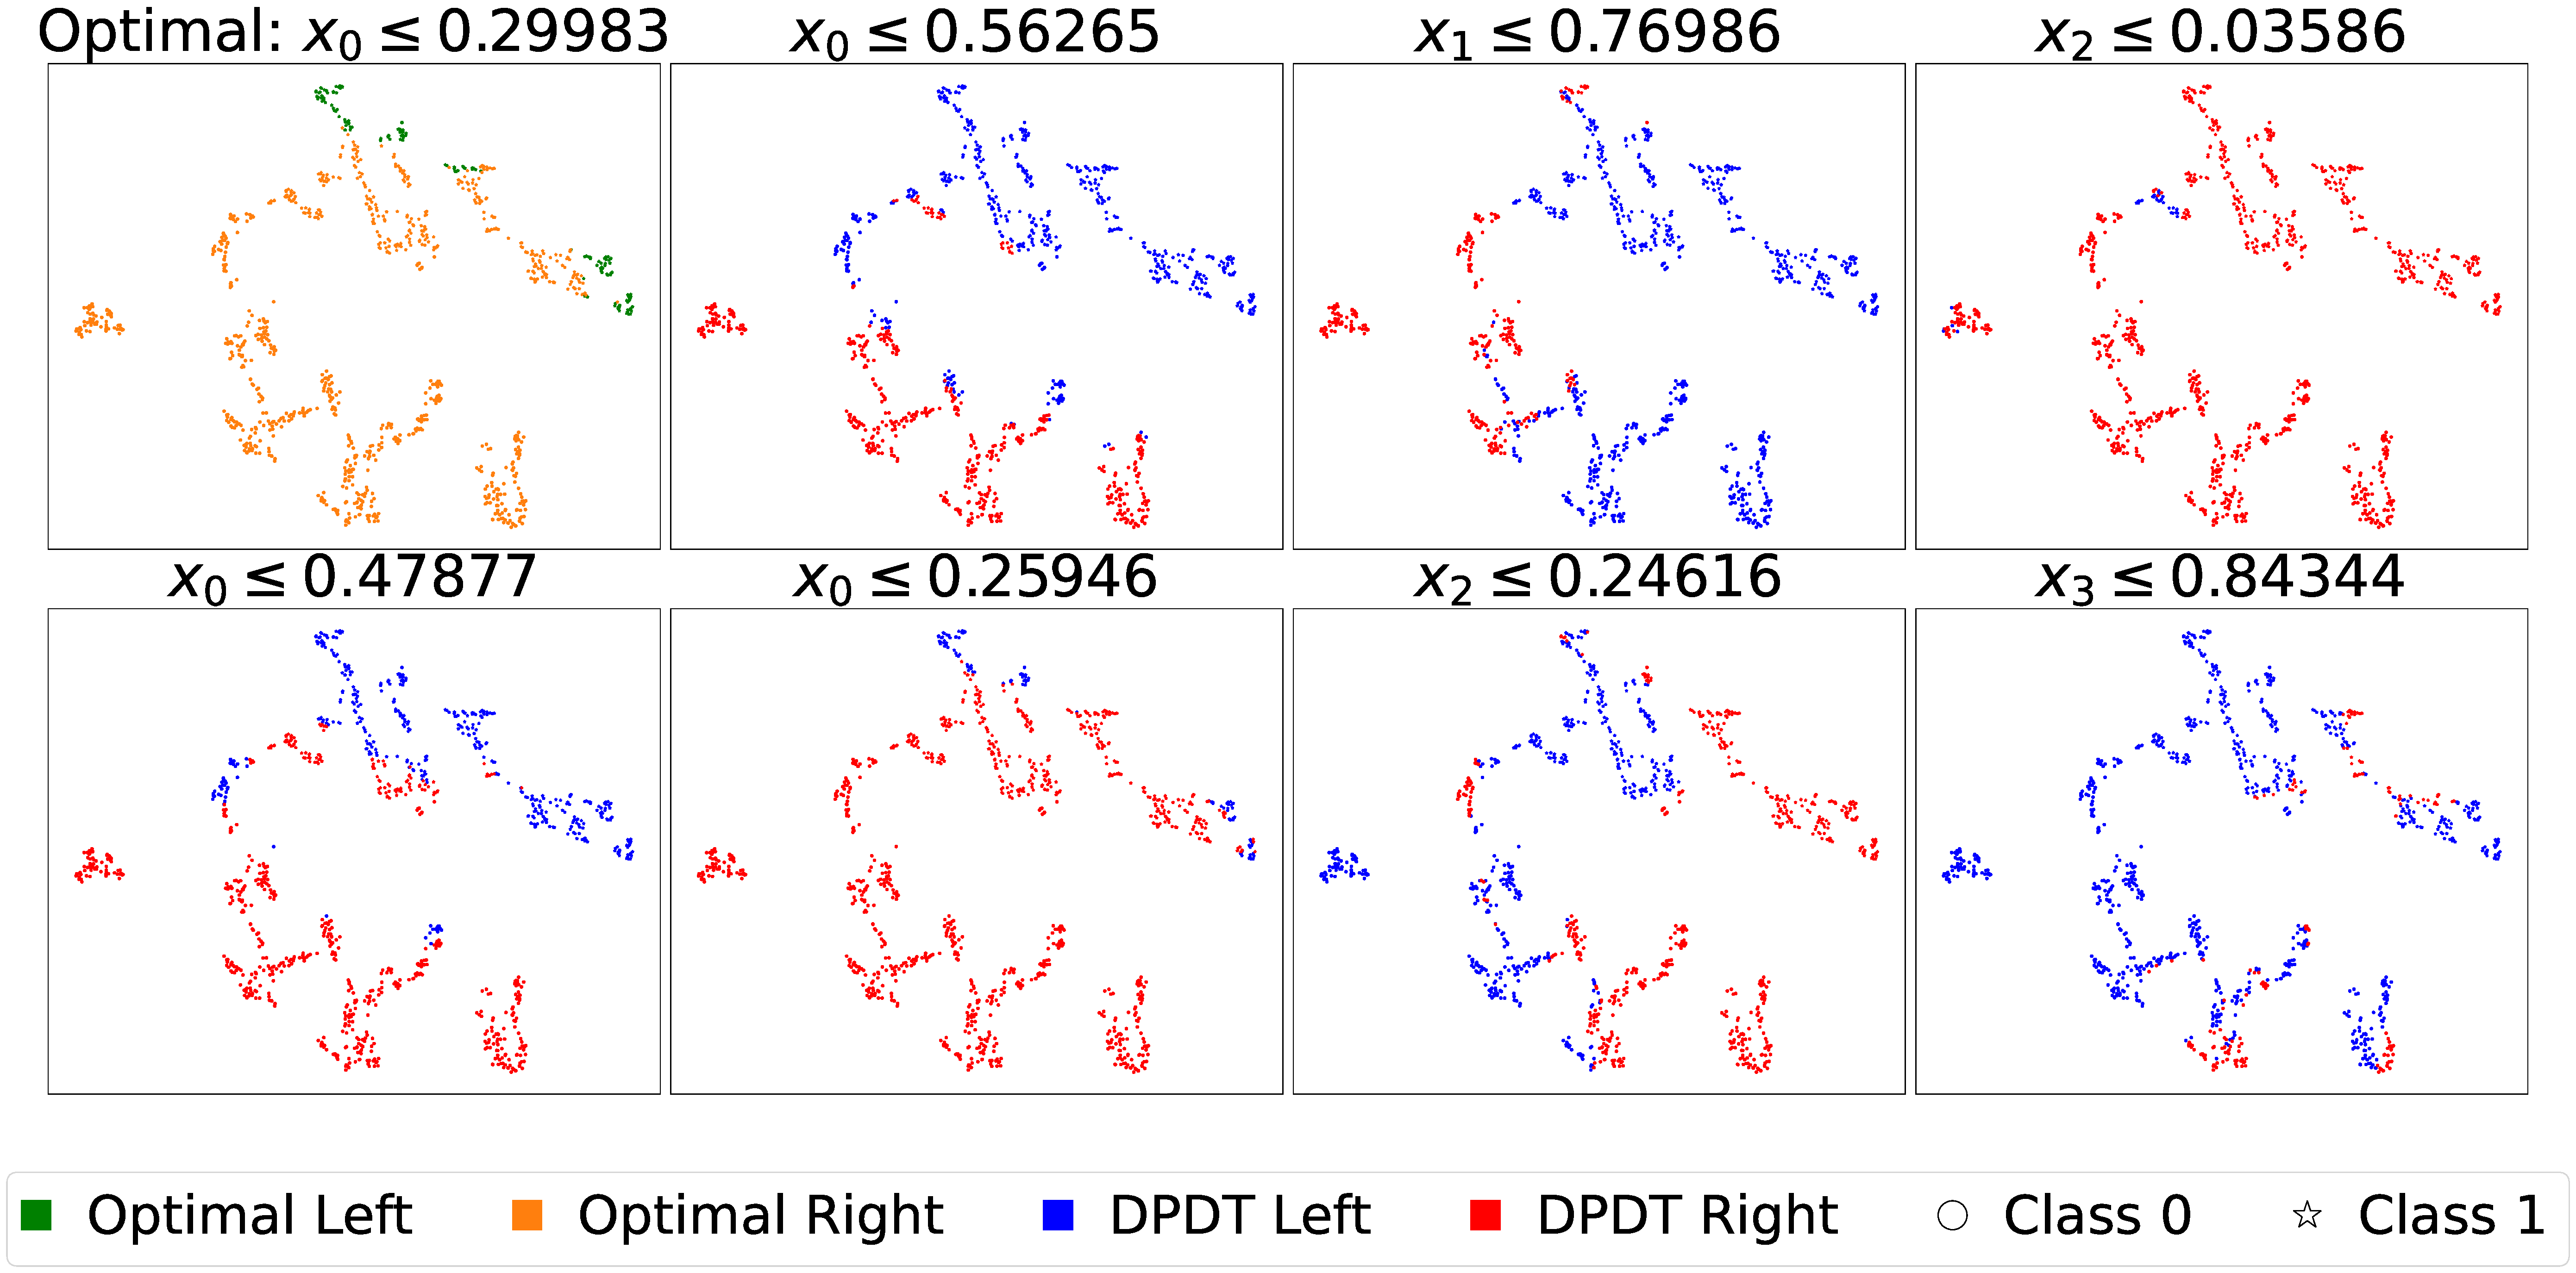
\includegraphics[width=1\linewidth]{images/figures/splits_tsne_combined.pdf}
    \caption{Root splits candidate obtained with DPDT compared to the optimal root split on the Bank dataset. Each split creates a partition of $p$-dimensional data that we projected in the $2$-dimensional space using t-SNE.}
    \label{fig:splits_dpdt}
\end{figure}
\begin{figure}
    \centering
    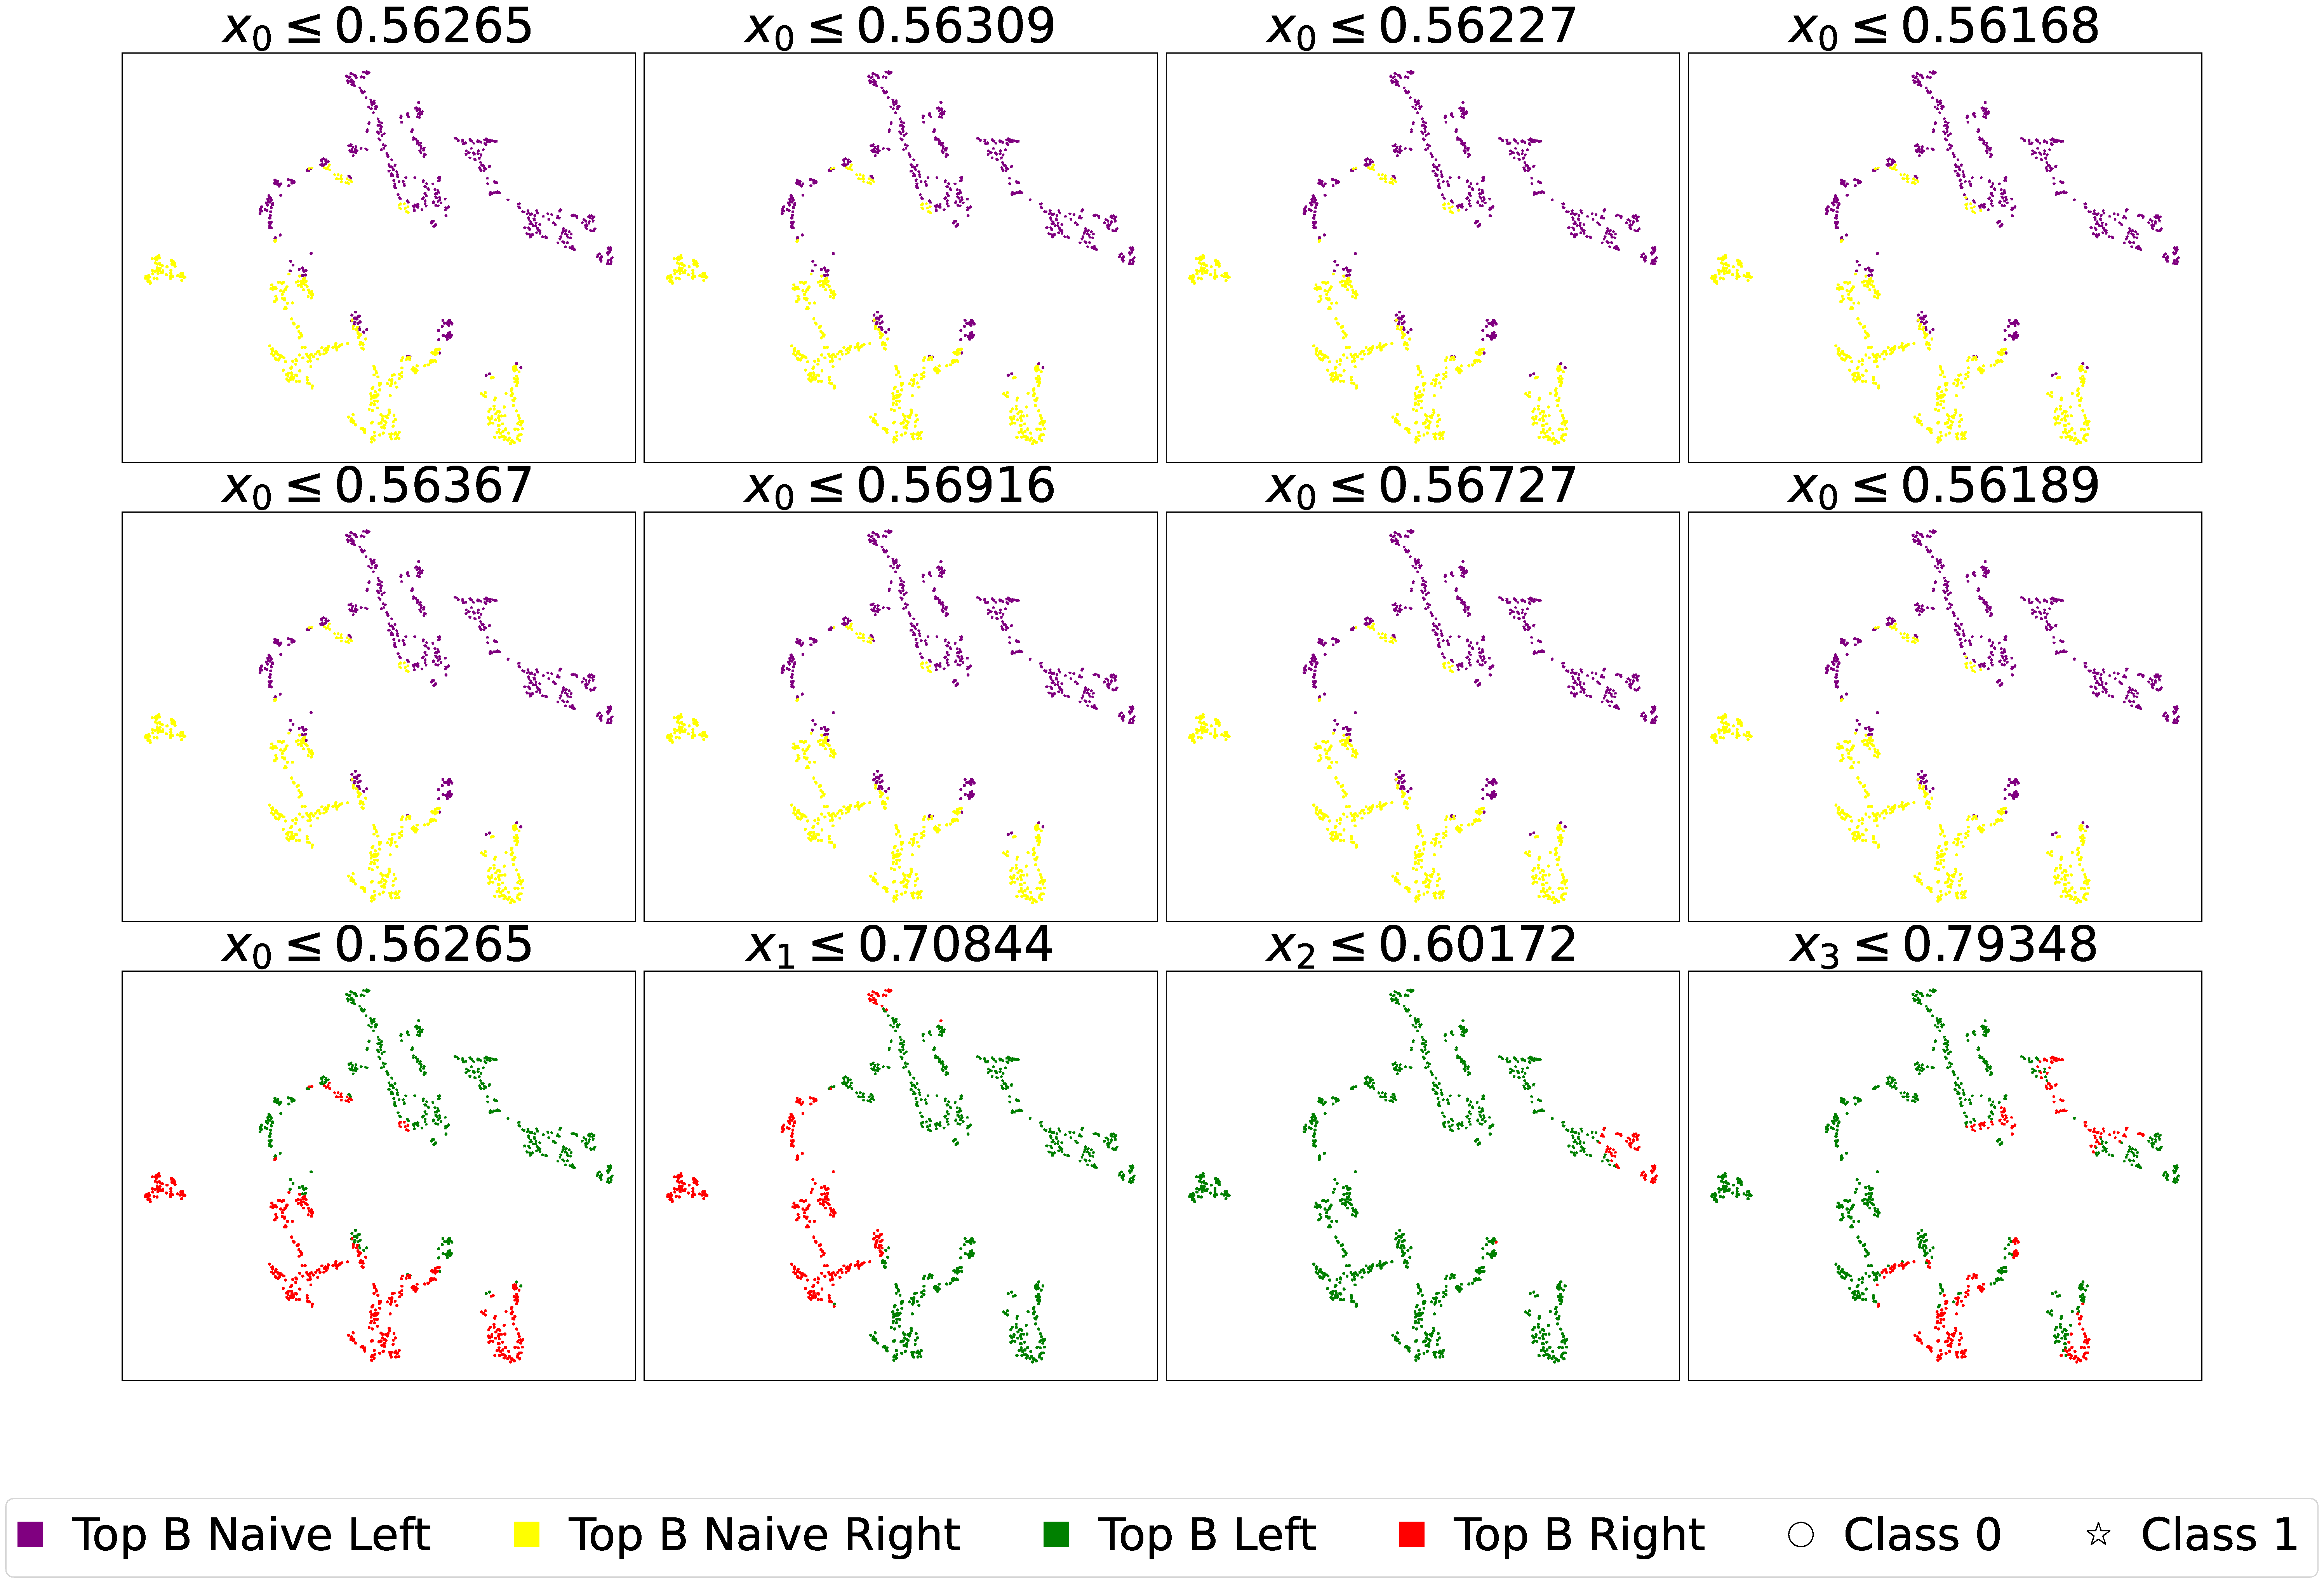
\includegraphics[width=1\linewidth]{images/figures/splits_tsne_combined_topk.pdf}
    \caption{Root splits candidate obtained with Top-B\cite{topk} on the Bank dataset. Each split creates a partition of $p$-dimensional data that we projected using t-SNE.}
    \label{fig:splits_topb}
\end{figure}

From an empirical perspective, it is key to evaluate DPDT training accuracy since optimal decision tree algorithms against which we wish to compare ourselves are designed to optimize the regularized training loss Eq.\ref{eq:suplearning}.

\subsection{Setup}
\paragraph{Metrics:} we are interested in the regularized training loss of algorithms optimizing Eq.\ref{eq:suplearning} with $\alpha=0$ and a maximum depth $D$. We are also interested in the number of key operations performed by each baseline, namely computing candidate split nodes for subsets of the training data. We disregard running times as solvers are implemented in different programming languages and/or using optimized code: operations count is more representative of an algorithm efficiency. We also qualitatively compare different decision trees root splits to some optimal root split.
\paragraph{Baselines:} we benchmark DPDT against greedy trees and optimal trees. For greedy trees we compare DPDT to CART \cite{breiman1984classification}. For optimal trees we compare DPDT to Quant-BnB \cite{quantbnb} which is the only solver specialized for depth 3 trees and continuous features. We also consider the non-greedy baseline Top-B \cite{topk}. Ideally, DPDT should have training accuracy close to the optimal tree while performing a number of operations close to the greedy algorithm. Furthermore, comparing DPDT to Top-B brings answers to which heuristic splits are better to consider. 

We use the CART algorithm implemented in \texttt{scikit-learn}~\cite{scikit-learn} in \texttt{CPython} with a maximum depth of 3. Optimal trees are obtained by running the \texttt{Julia} implementation of the Quant-BnB solver from~\cite{quantbnb} specialized in depth 3 trees for datasets with continuous features. We use a time limit of 24 hours per dataset. 
DPDT and Top-B trees are obtained with algorithm~\ref{alg:dpdt} implemented in pure \texttt{Python} and the calls to CART and Top-B most informative splits generating functions from section~\ref{sec:the-mdp} respectively.
We use the modified DQN from section~\ref{sec:topin} on classification POIBMDPs with $\zeta=1$ (we want to learn the best tree possible disregarding interpretability) and maximum depth control using rewards or termination signals.
\paragraph{Datasets:} we us the same datasets as the Quant-BnB paper~\cite{quantbnb}.

\subsection{Observations}

\paragraph{Near-optimality} Our experimental results demonstrate that unlike Deep RL, DPDT and Top-B approaches consistently improve upon greedy solutions while requiring significantly fewer operations than exact solvers. Looking at Table~\ref{tab:tree_comparison_combined}, we observe several key patterns:
first, light DPDT with 16 candidate root splits consistently outperforms the greedy baseline in all datasets. This shows that in practice DPDT can be strictly netter than CART outside of theorem \ref{thm:better_greedy} assumptions. 
Second, when comparing DPDT to Top-B, we see that DPDT generally achieves better accuracy for the same configuration. For example, on the bean dataset, full DPDT reaches 85.3\% accuracy while full Top-B achieves 84.1\%. This pattern holds on most datasets, suggesting that DPDT is more effective than selecting splits based purely on information gain.


Third, both approaches achieve impressive computational efficiency compared to exact solvers. While optimal solutions require between $10^4$ to $10^8$ operations, DPDT and Top-B typically need only $10^2$ to $10^4$ operations, a reduction of 2 to 4 orders of magnitude.
Notably, on several datasets (room, avila, occupancy, bidding), full DPDT matches or comes extremely close to optimal accuracy while requiring far fewer operations. For example, on the room dataset, full DPDT achieves the optimal accuracy of 99.2\% while reducing operations from $1.34\times10^6$ to $1.61\times10^4$.
These results demonstrate that DPDT provides an effective middle ground between greedy approaches and exact solvers, offering near-optimal solutions with reasonable computational requirements. While both DPDT and Top-B improve upon greedy solutions, DPDT CART-based split generation strategy appears to be particularly effective at finding high-quality solutions.

\paragraph{DPDT splits} To understand why the CART-based split generation yields more accurate DPDT trees than the Top-B heuristic, we visualize how splits partition the feature space (figures \ref{fig:splits_dpdt}, \ref{fig:splits_topb}). We run both DPDT with splits from CART and DPDT with the Top-B most informative splits on the bank dataset. We use t-SNE to create a two-dimensional representations of the dataset partitions given by candidates root splits from CART and Top-B. 
The optimal root split for the depth-3 tree for bank--obtained with Quant-BnB--is shown on figure \ref{fig:splits_dpdt} in the top-left subplot using green and orange colors for the resulting partitions. On the same figure we can see that the DPDT split generated with CART $x_0 \leq 0.259$ is very similar to the optimal root split. However, on figure \ref{fig:splits_topb} we observe that no Top-B candidate splits resemble the optimal root and that in general Top-B split lack diversity: they always split along the same feature. We tried to enforce diversity by getting the most informative split \textit{per feature} but no candidate split resembles the optimal root.

\section{DPDT generalization capabilities}\label{sec:generalization}
\begin{figure}
    \centering
    \begin{minipage}{0.24\textwidth}
        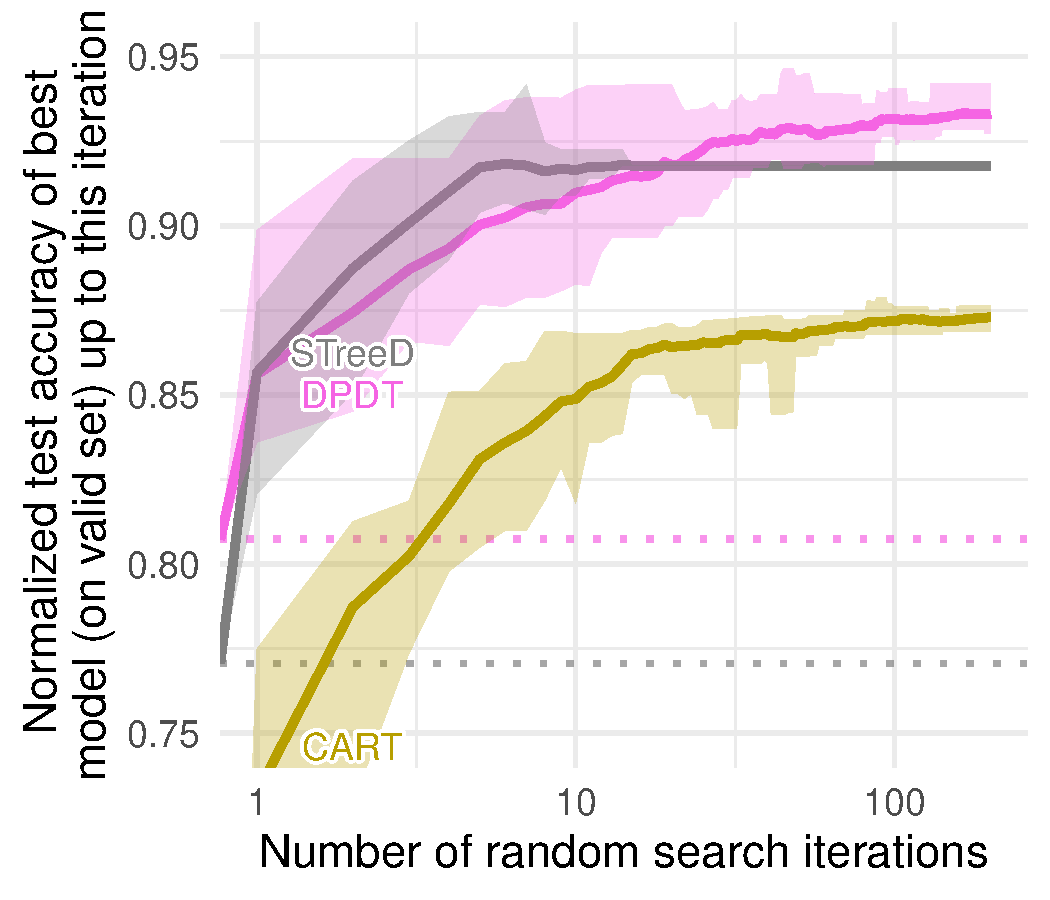
\includegraphics[width=\textwidth]{images/figures/tab_bench/random_search_classif_numerical_depth5.pdf}
        \subcaption{Single Tree Numerical}\label{fig:gen-num}
    \end{minipage}
    \begin{minipage}{0.24\textwidth}
        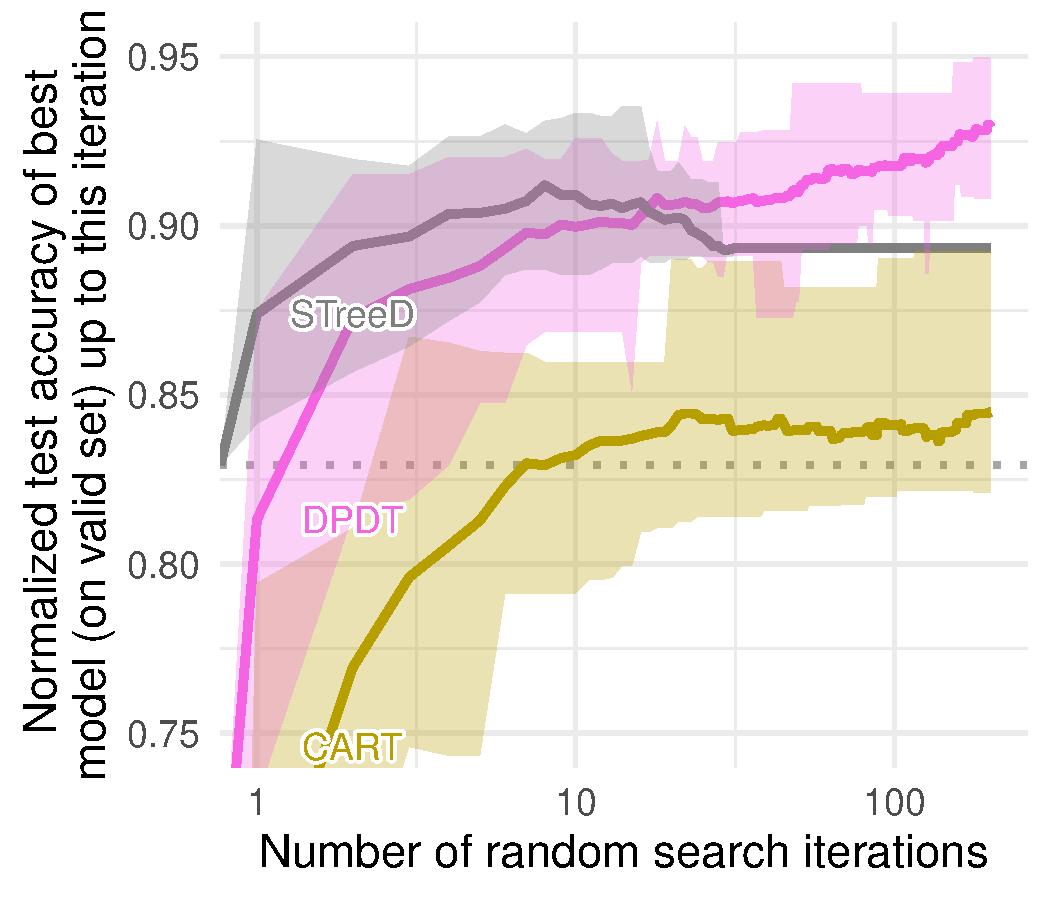
\includegraphics[width=\textwidth]{images/figures/tab_bench/random_search_classif_categorical_depth5.pdf}
        \subcaption{Single Tree Categorical}\label{fig:gen-cat}
    \end{minipage}
        \centering
    \begin{minipage}{0.24\textwidth}
        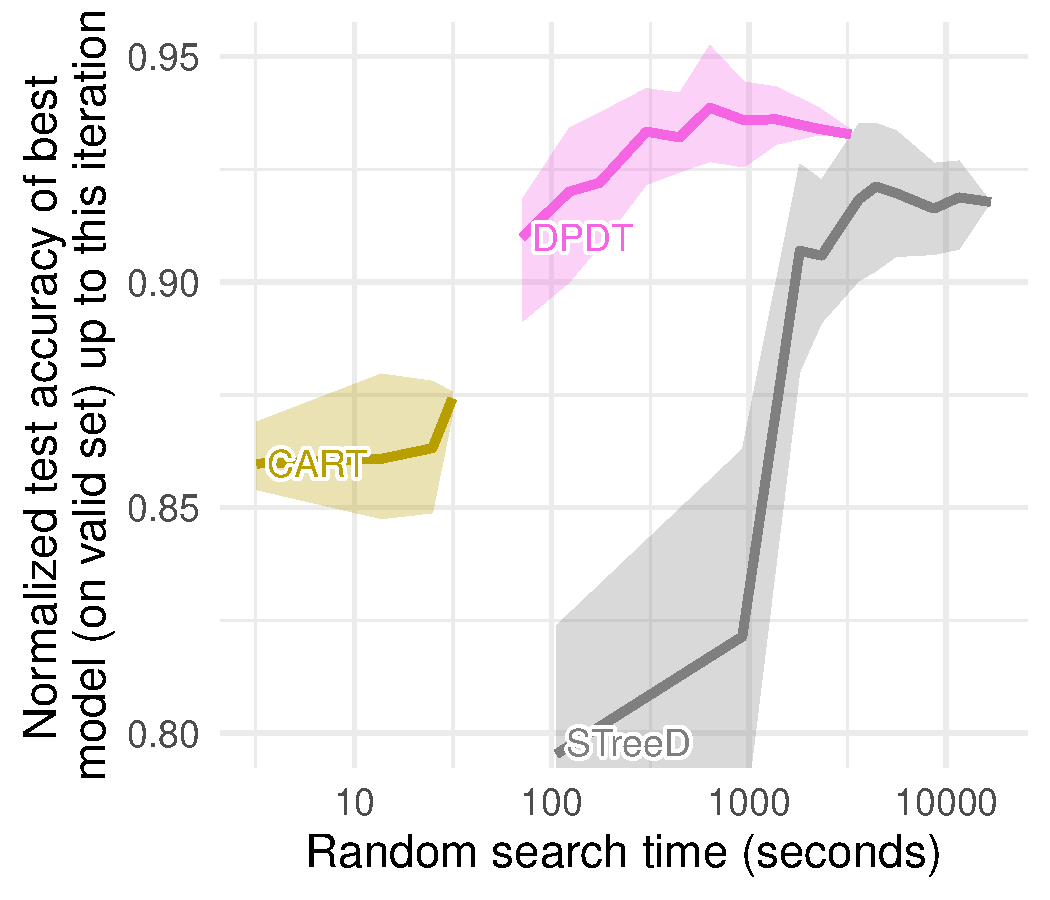
\includegraphics[width=\textwidth]{images/figures/tab_bench/benchmark_time_numerical_classif.pdf}
        \subcaption{Single Tree Numerical}\label{fig:gen-num-time}
    \end{minipage}
    \begin{minipage}{0.24\textwidth}
        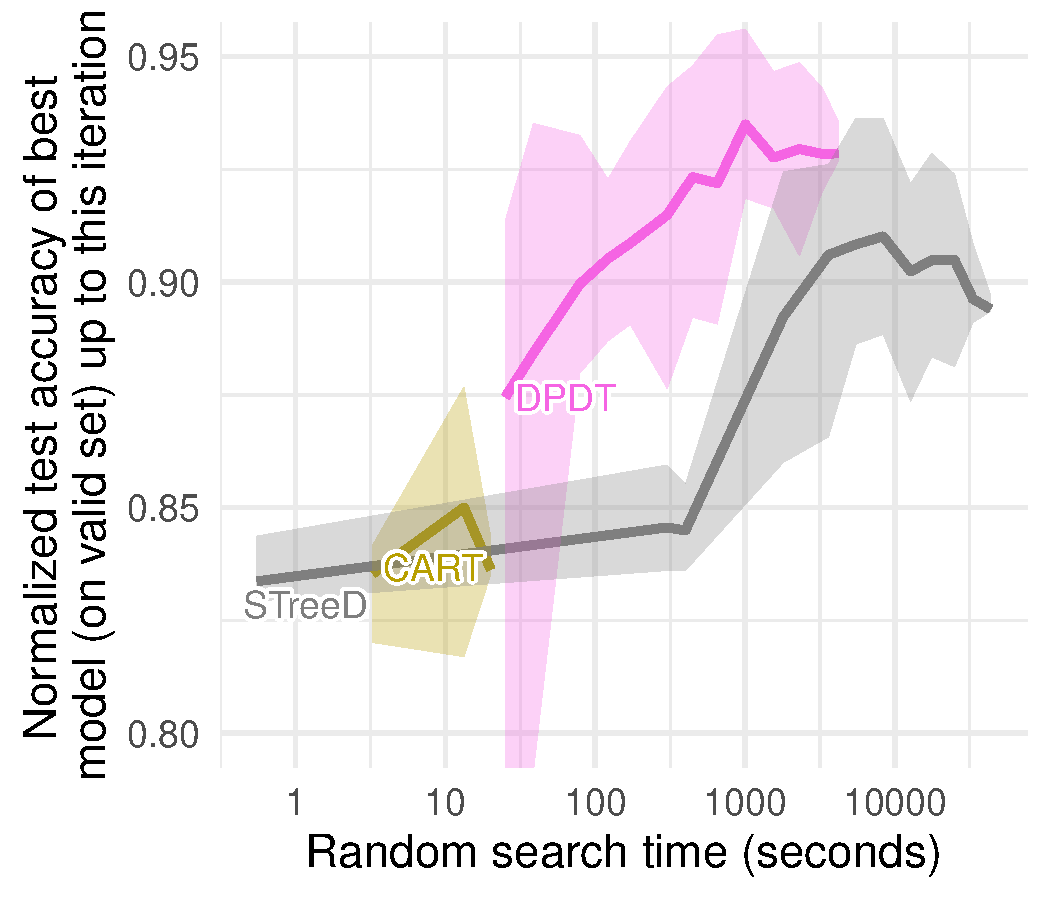
\includegraphics[width=\textwidth]{images/figures/tab_bench/benchmark_time_categorical_classif.pdf}
        \subcaption{Single Tree Categorical}\label{fig:gen-cat-time}
    \end{minipage}
          \begin{minipage}{0.24\textwidth}
          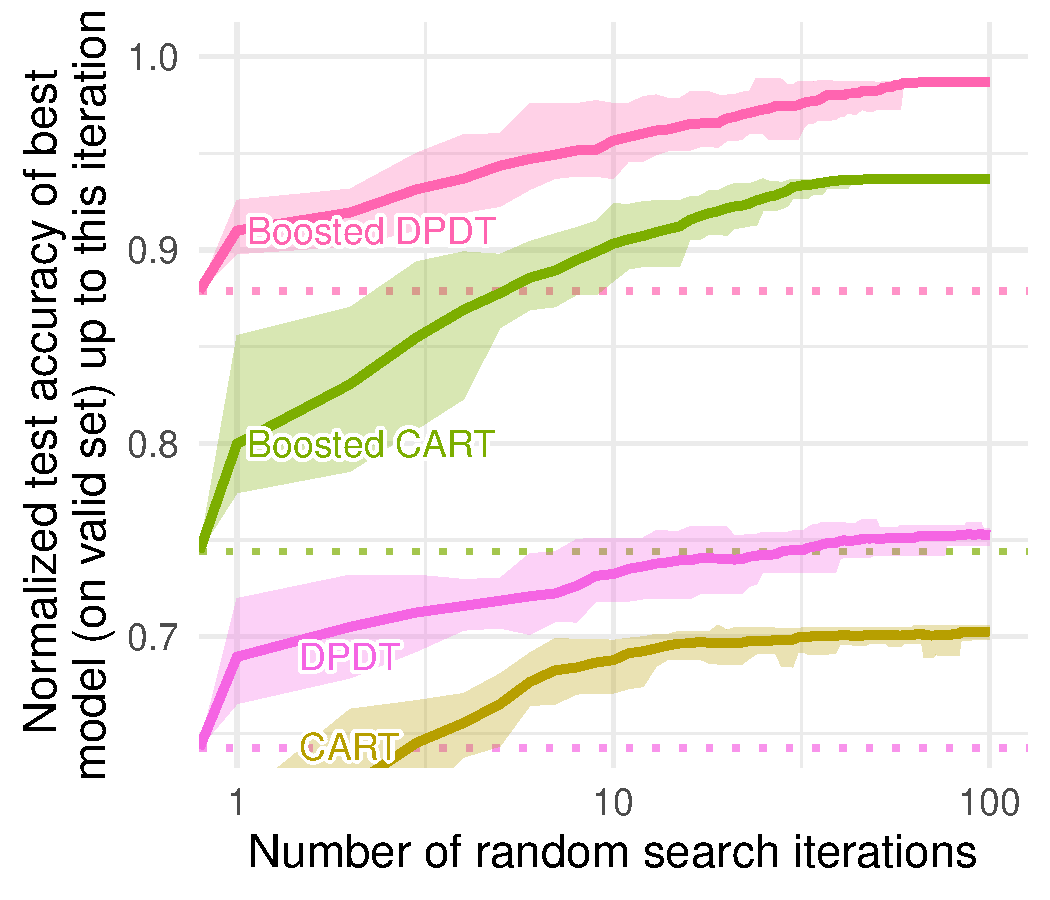
\includegraphics[width=\textwidth]{images/figures/tab_bench/random_search_classif_numerical_boosting_w_weak.pdf}
          \subcaption{Boosting vs Single Tree Num.}\label{fig:boost-num}
      \end{minipage}
      \begin{minipage}{0.24\textwidth}
          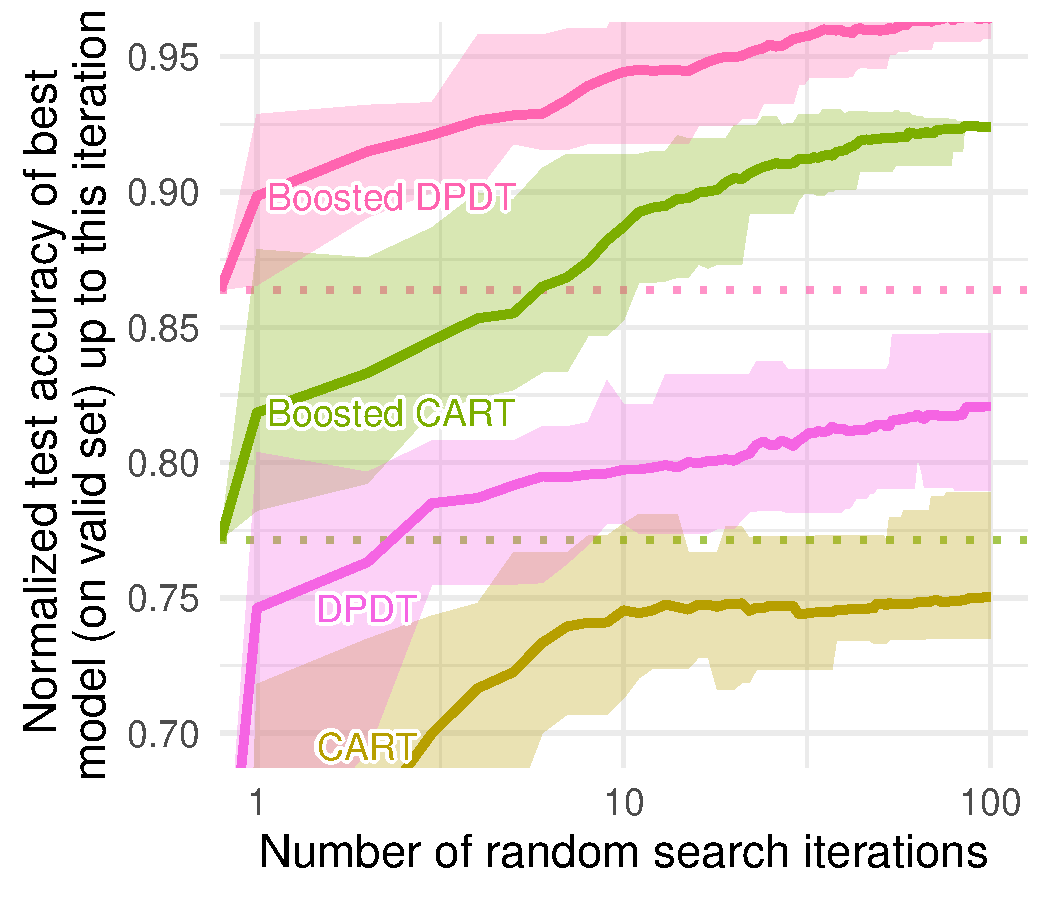
\includegraphics[width=\textwidth]{images/figures/tab_bench/random_search_classif_categorical_boosting_w_weak.pdf}
          \subcaption{Boosting vs Single Tree Cat.}\label{fig:boost-cat}
      \end{minipage}
    \centering
    \begin{minipage}{0.24\textwidth}
        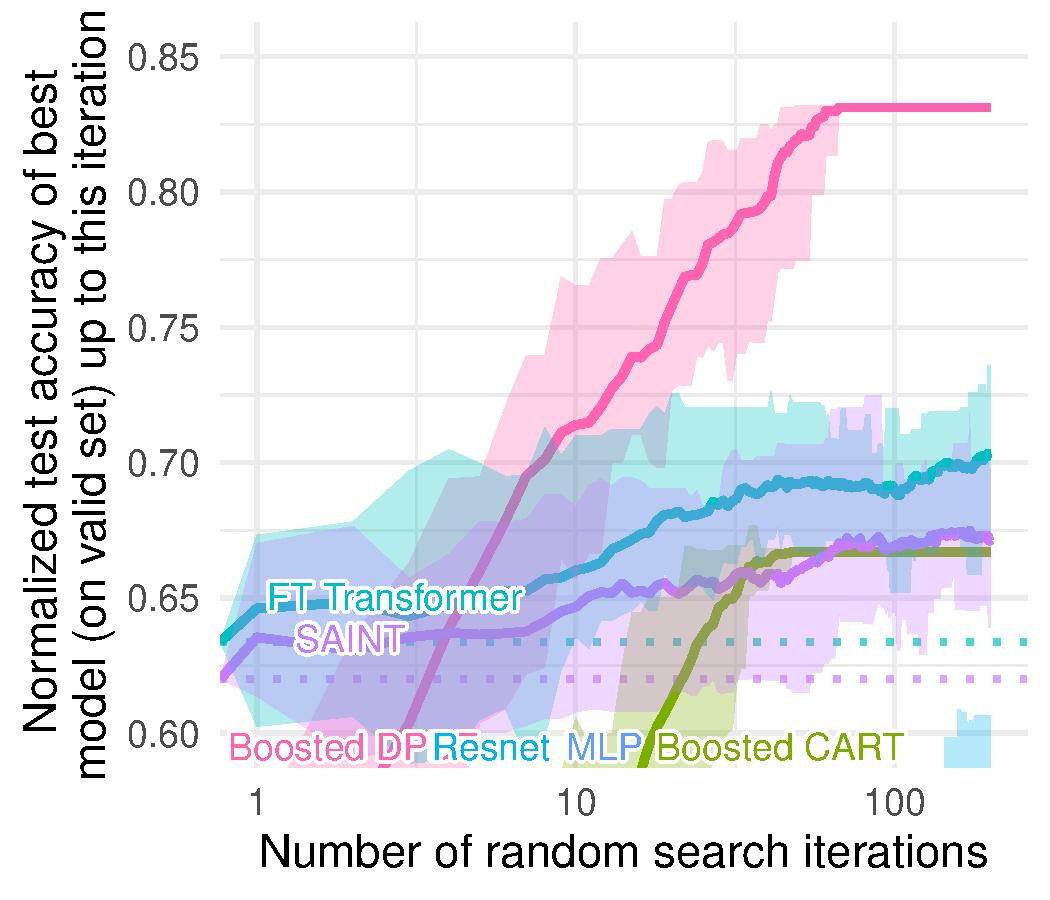
\includegraphics[width=\textwidth]{images/figures/tab_bench/random_search_classif_numerical_boosting_all_notgb.pdf}
        \subcaption{Boosting vs Neural Numerical}\label{fig:classif-num-all}
    \end{minipage}
    \begin{minipage}{0.24\textwidth}
        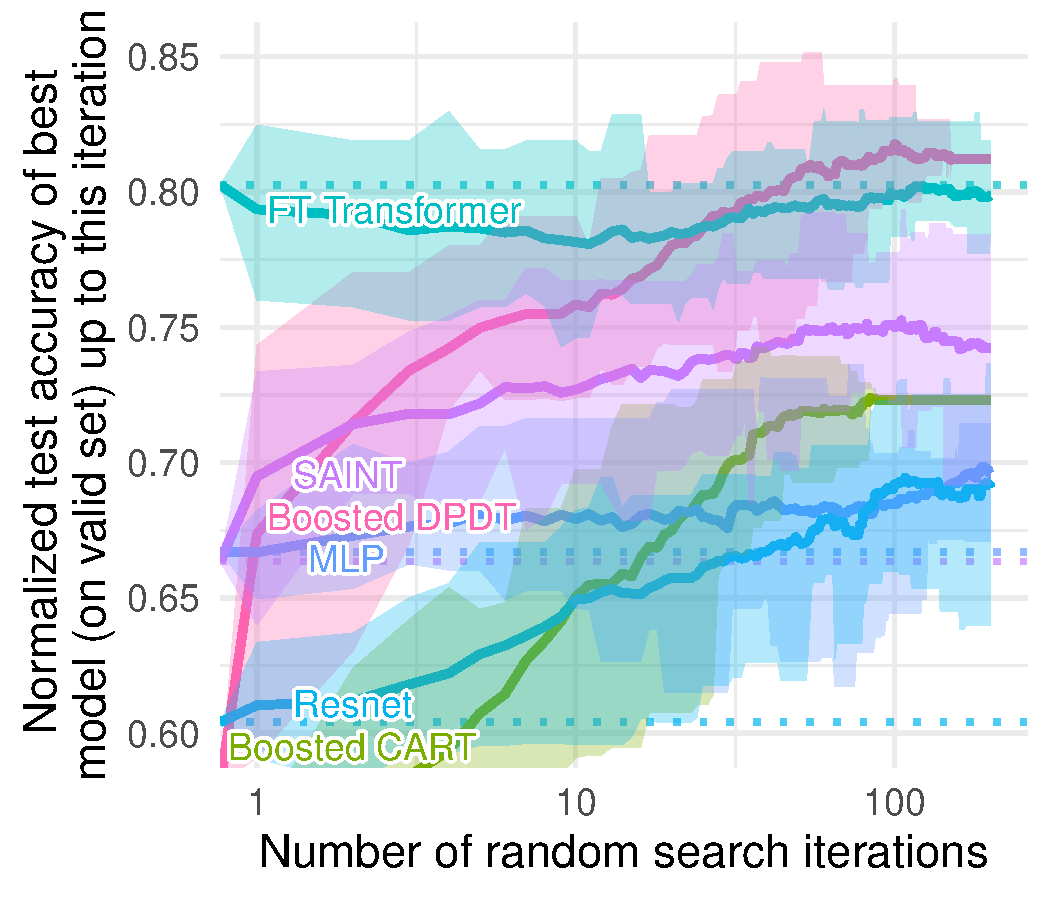
\includegraphics[width=\textwidth]{images/figures/tab_bench/random_search_classif_categorical_boosting_all_notgb.pdf}
        \subcaption{Boosting vs Neural Categorical}\label{fig:classif-cat-all}
    \end{minipage}
\caption{Benchmark on medium-sized datasets. Dotted lines correspond to the score of the default hyperparameters, which is also the first random search iteration. Each value corresponds to the test score of the best model (obtained on the validation set) after a specific number of random search iterations (a, b) or after a specific time spent doing random search (c, d), averaged on 15 shuffles of the random search order. The ribbon corresponds to the minimum and maximum scores on these 15 shuffles.}\label{fig:gen-classif}
\end{figure}

The goal of this section is to have a fair comparison of generalization capabilities of different tree induction algorithms. Fairness of comparison should take into account the number of hyperparameters, choice of programming language, intrinsic purposes of each algorithms (what are they designed to do?), the type of data they can read (categorical features or numerical features). We benchmark DPDT using~\cite{grinsztajn2022tree}. We choose this benchmark because it was used to establish XGBoost~\cite{xgb} as the SOTA tabular learning model. 

\subsection{Setup}

\paragraph{Metrics:} We re-use the code from \cite{grinsztajn2022tree}~\footnote{https://github.com/leogrin/tabular-benchmark}. It relies on random searches for hyper-parameter tuning \cite{pmlr-v28-bergstra13}. We run a random search of 100 iterations per dataset for each benchmarked tree algorithms. To study performance as a function of the number $n$ of random search iterations, we compute the best hyperparameter combination on the validation set on these $n$ iterations (for each model and dataset), and evaluate it on the test set. Following \cite{grinsztajn2022tree}, we do this 15 times while shuffling the random search order at each time. This gives us bootstrap-like estimates of the expected test score of the best tree found on the validation set after each number of random search iterations. In addition, we always start the random searches with the default hyperparameters of each tree induction aglorithm. We use the test set accuracy (classification) to measure model performance. The aggregation metric is discussed in details in \cite[section 3]{grinsztajn2022tree}.

\paragraph{Datasets:} we use the datasets curated by \cite{grinsztajn2022tree}. They are available on \texttt{OpenML} \cite{10.1145/2641190.2641198} and described in details in \cite[appendix A.1]{grinsztajn2022tree}. The attributes in these datasets are either %Those datasets are either 
numerical (a real number), or categorical (a symbolic values among a finite set of possible values). %,  strings as well as numbers). 
The considered datasets follow a strict selection \cite[section 3]{grinsztajn2022tree} to focus on core learning challenges. Some datasets are very large (millions of samples) like Higgs or Covertype \cite{higgs_280,covertype_31}. To ensure non-trivial learning tasks, datasets where simple models (e.g.\@ logistic regression) performed within 5\% of complex models (e.g.\@ ResNet~\cite{resnet}, HistGradientBoosting~\cite{scikit-learn}) are removed. We use the same data partitioning strategy as~\cite{grinsztajn2022tree}: 70\% of samples are allocated for training, with the remaining 30\% split between validation (30\%) and test (70\%) sets. Both validation and test sets are capped at 50,000 samples for computational efficiency. All algorithms and hyperparameter combinations were evaluated on identical folds. Finally, while we focus on classification datasets in the main text, we provide results for regression problems in table~\ref{tab:regression} in the appendix.

\paragraph{Baselines:}
we benchmark DPDT against CART and STreeD when inducing trees of depth at most 5.  We use hyperparameter search spaces from \cite{komer-proc-scipy-2014} for CART and DPDT. For DPDT we additionally consider eight different splits functions parameters configurations for the maximum nodes in the calls to CART. Surprisingly, after computing the importance of each hyperparameter of DPDT, we found that the maximum node numbers in the calls to CART are only the third most important hyperparametrer behind classical ones like the minimum size of leaf nodes or the minimum impurity decrease (Table~\ref{tab:importance_comparison}). We use the \texttt{CPython} implementation of STreeD\footnote{PySTreeD: \url{https://github.com/AlgTUDelft/pystreed}}. All hyperparameter grids are given in table \ref{tab:tree_hyperparams} in the appendix.

\paragraph{Hardware:} experiments were conducted on a heterogeneous computing infrastructure made of AMD EPYC 7742/7702 64-Core and Intel Xeon processors, with hardware allocation based on availability and algorithm requirements. DPDT and CART random searches ran for the equivalent of 2-days while \texttt{PySTreeD} ran for 10-days.

\begin{table}
\centering
\small
\caption{Hyperparameters importance comparison. A description of the hyperparameters can be found in the scikit-learn documentation: \url{https://scikit-learn.org/stable/modules/generated/sklearn.tree.DecisionTreeClassifier.html}.}
\begin{tabular}{lccc}
\toprule
\textbf{Hyperparameter} & \textbf{DPDT (\%)}  & \textbf{CART (\%)} & \textbf{STreeD (\%)} \\
\midrule
min\_samples\_leaf & 35.05 & 33.50 & 50.50 \\
min\_impurity\_decrease & 24.60 & 24.52 & - \\
cart\_nodes\_list & 15.96 & - & - \\
max\_features & 11.16 & 18.06 & - \\
max\_depth & 7.98 & 10.19 & 0.00 \\
max\_leaf\_nodes & - & 7.84 & - \\
min\_samples\_split & 2.67 & 2.75 & - \\
min\_weight\_fraction\_leaf & 2.58 & 3.14 & - \\
max\_num\_nodes & - & - & 27.51 \\
n\_thresholds & - & - & 21.98 \\
\bottomrule
\end{tabular}
\label{tab:importance_comparison}
\end{table}

\subsection{Observations}

\paragraph{Generalization} In figure \ref{fig:gen-classif}, we observe that DPDT learns better trees than CART and STreeD both in terms of generalization capabilities and in terms of computation cost. On figures \ref{fig:gen-num} and \ref{fig:gen-cat}, DPDT obtains best generalization scores for classification on numerical and categorical data after 100 iterations of random hyperparameters search over both CART and STreeD. Similarly, we also present generalization scores as a function of compute time (instead of random search iterations). On figures \ref{fig:gen-num-time} and \ref{fig:gen-cat-time}, despite being coded in the slowest language (\texttt{Python} vs. \texttt{CPython}), our implementation of DPDT finds the best overall model before all STreeD random searches even finish.
The results from figure \ref{fig:gen-classif} are appealing for machine learning practitioners and data scientists that have to do hyperparameters search to find good models for their data while having computation constrains.

Now that we have shown that DPDT is extremely efficient to learn shallow decision trees that generalize well to unseen data, it is fair to ask if DPDT can also learn deep trees on very large datasets.

\begin{table}
\centering
\caption{Depth-10 decision trees for the KDD 1999 cup dataset.}
\label{tab:model-comparison}
\small
\begin{tabular}{lccc}
\hline
\textbf{Model} & \textbf{Test Accuracy (\%)} & \textbf{Time (s)} & \textbf{Memory (MB)} \\
\hline
DPDT-(4,) & \textbf{91.30} & 339.85 & 5054 \\
DPDT-(4,4,) & \textbf{91.30} & 881.07 & 5054 \\
CART & 91.29 & 25.36 & 1835 \\
GOSDT-$\alpha=0.0005$& 65.47 & 5665.47 & 1167 \\
GOSDT-$\alpha=0.001$ & 65.45 & 5642.85 & 1167 \\
\hline
\end{tabular}
\end{table}

\paragraph{Deeper trees on bigger datasets} We also stress test DPDT by inducing deep trees of depth 10 for the KDD 1999 cup dataset\footnote{\url{http://kdd.ics.uci.edu/databases/kddcup99/kddcup99.html}}. The training set has 5 million rows and a mix of 80 continuous and categorical features representing network intrusions. We fit DPDT with 4 split candidates for the root node (DPDT-(4,)) and with 4 split candidates for the root and for each of the internal nodes at depth 1 (DPDT-(4,4,)). We compare DPDT to CART with a maximum depth of 10 and to GOSDT\footnote{Code available at: \url{https://github.com/ubc-systopia/gosdt-guesses}}~\cite{mctavish2022fast} with different regularization values $\alpha$. GOSDT first trains a tree ensemble to binarize a dataset and then solve for the optimal decision tree of depth 10 on the binarized problem. In Table~\ref{tab:model-comparison} we report the test accuracy of each tree on the KDD 1999 cup test set. We also report the memory peak during training and the training duration (all experiments are run on the same CPU). We observe that DPDT can improve over CART even for deep trees and large datasets while using reasonable time and memory. Furthermore, Table \ref{tab:model-comparison} highlights the limitation of optimal trees for practical problems when the dataset is not binary. We observed that GOSDT could not find a good binarization of the dataset even when increasing the budget of the tree ensemble up to the point where most of the computations are spent on fitting the ensemble (see more details about this phenomenon in \cite[section 5.3]{mctavish2022fast}). In table \ref{tab:more-res} in the appendix, we also show that DPDT performs better than optimal trees for natively binary datasets. In the next section we study the performance of boosted DPDT trees.

\section{Application of DPDT to Boosting}

In the race for machine learning algorithms for tabular data, boosting procedures are often considered the go-to methods for classification and regression problems. Boosting algorithms \cite{FREUND1997119,stcohFriedman,FriedmanBoosting} sequentially add weak learners to an ensemble called strong learner. The development of those boosting algorithms has focused on what data to train newly added weak learners \cite{stcohFriedman,FriedmanBoosting},  or on efficient implementation of those algorithms \cite{xgb,10.5555/3327757.3327770}. We show next that Boosted-DPDT (boosting DPDT trees with AdaBoost \cite{FREUND1997119}) improves over recent deep learning algorithms. 

\subsection{Boosted-DPDT}\label{sec:boosting}

We benchmark Boosted-DPDT with the same datasets, metrics, and hardware as in the previous section on single-tree training. Second, we verify the competitiveness of Boosted-DPDT with other models such as deep learning ones (SAINT~\cite{somepalli2021saintimprovedneuralnetworks} and other deep learning architectures from \cite{resnet}). 

On figures \ref{fig:boost-num} and \ref{fig:boost-cat} we can notice 2 properties of DPDT. First, as in any boosting procedure, Boosted-DPDT outperforms its weak counterpart DPDT. This serves as a sanity check for boosting DPDT trees. Second, it is clear that boosting DPDT trees yields better models than boosting CART trees on both numerical and categorical data. figures~\ref{fig:classif-num-all} and \ref{fig:classif-cat-all} show that boosting DPDT trees using the default AdaBoost procedure~\cite{FREUND1997119} is enough to learn models outperforming deep learning algorithms on datasets with numerical features and models in the top-tier on datasets with categorical features. This show great promise for models obtained when boosting DPDT trees with more advanced procedures.

\subsection{(X)GB-DPDT}
\begin{figure}
    \centering
    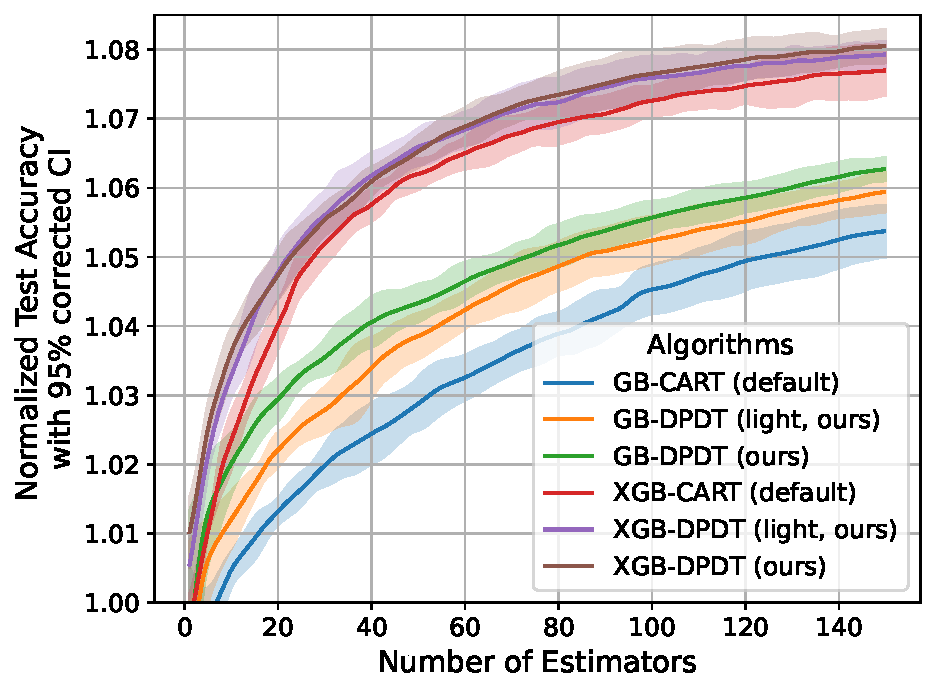
\includegraphics[trim={0 0 0 0},clip,width=0.6\linewidth]{images/figures/xgboosting_normalized_wo_opt.pdf}
    \caption{Aggregated mean test accuracies of Gradient Boosting models as a function of the number of single trees.}
    \label{fig:gb}
\end{figure}

We also boost DPDT trees with Gradient Boosting and eXtreme Gradient Boosting~\cite{FriedmanBoosting,stcohFriedman,xgb}(X(GB)-DPDT). For each dataset from~\cite{grinsztajn2022tree}, we trained (X)GB-DPDT models with 150 boosted single DPDT trees and a maximum depth of 3 for each. We evaluate two DPDT configurations for the single trees: light (DPDT-(4, 1, 1)) and the default (DPDT-(4,4,4)). We compare (X)GB-DPDT to (X)GB-CART: 150 boosted CART trees with maximum depth of 3 and default hyperparameters for each. All models use a learning rate of 0.1. For each each dataset, we normalize all boosted models scores by the accuracy of a single depth-3 CART decision tree and aggregate the results: the final curves represent the mean performance across all datasets, with confidence intervals computed using 5 different random seeds.

figure~\ref{fig:gb} shows that similarly to simple boosting procedures like AdaBoost, more advanced ones like (eXtreme) Gradient Boosting yields better models when the weak learners are DPDT trees rather than greedy trees. This is a motivation to develop efficient implementation of (eXtreme) Gradient Boosting with DPDT as the weak learning algorithm to perform extensive benchmarking following \cite{grinsztajn2022tree} and potentially claim the state-of-the-art.



\section{Conclusion}\label{sec:ccl-dpdt}

In this part of the manuscript, we introduced Dynamic Programming Decision Trees (DPDT), a novel framework that bridges the gap between greedy and optimal decision tree algorithms. By formulating tree induction as an MDP and employing adaptive split generation based on CART, DPDT achieves near-optimal training loss with significantly reduced computational complexity compared to existing optimal tree solvers. Furthermore, we prove that DPDT can learn strictly more accurate trees than CART. 
Most importantly, extensive benchmarking on varied large and difficult enough datasets showed that DPDT trees and boosted DPDT trees generalize better than other baselines. To conclude, we showed that DPDT is a promising machine learning algorithm. 

The key future work would be to make DPDT industry-ready by implementing it in \texttt{C} and or making it compatible with the most advanced implementation of e.g.\@ XGBoost.
While DPDT is designed for supervised learning (\ref{sec:dl}), an other interesting future work direction could be to use DPDT in the tree induction routine of imitation learning algorithms like VIPER (algorithm~\ref{alg:viper},~\cite{viper}).
This could lean to better decision tree policy learning for the RL objective (\ref{def:mdp-obj}).

In the next and final part of this manuscript, we circle back to our original sequential decision making problems.
We will move away from \textit{learning} and focus on evaluating the interpretability-performance trade-offs of different policy class from figure~\ref{fig:performance-interpretability-trade-off}.



\part{Beyond Decision Trees: what can be done with other Interpretable Policies?}
%
% Quatrième chapitre
%
% Cinquième chapitre
%
% Sixième chapitre
%
% Chapitre  de conclusion (générale)
%%%%%%%%%%%%%%%%%%%%%%%%%%%%%%%%%%%%%%%%%%%%%%%%%%%%%%%%%%%%%%%%%%%%%%%%%%%%%%%
\chapter*{Conclusion générale}

%
% Liste des références bibliographiques
\printbibliography
%
%%%%%%%%%%%%%%%%%%%%%%%%%%%%%%%%%%%%%%%%%%%%%%%%%%%%%%%%%%%%%%%%%%%%%%%%%%%%%%%
% Début de la partie annexe éventuelle
%%%%%%%%%%%%%%%%%%%%%%%%%%%%%%%%%%%%%%%%%%%%%%%%%%%%%%%%%%%%%%%%%%%%%%%%%%%%%%%
\appendix
%
% Deuxième chapitre annexe (éventuel)
\chapter{Programmes informatiques}
\label{chap-listings}

Les listings suivants sont au cœur de notre travail.

\lstinputlisting[caption={Il est l'heure}]{annexes/programmes/heure.c}
\lstinputlisting[caption={Factorielle}]{annexes/programmes/factorielle.c}


%
%%%%%%%%%%%%%%%%%%%%%%%%%%%%%%%%%%%%%%%%%%%%%%%%%%%%%%%%%%%%%%%%%%%%%%%%%%%%%%%
% Début de la partie finale
%%%%%%%%%%%%%%%%%%%%%%%%%%%%%%%%%%%%%%%%%%%%%%%%%%%%%%%%%%%%%%%%%%%%%%%%%%%%%%%
\backmatter
%
% (Facultatif) Glossaire (si souhaité distinct de la liste des acronymes) :
% \printglossary
%
% (Facultatif) Index :
% \printindex
%
% Table des matières
\tableofcontents
%
% (Facultatif) Production de la 4e de couverture :
% \makebackcover
%
\end{document}